\documentclass[%
%parskip,
german,
titlepage=firstiscover,
fontsize=12pt,
twoside=true,
listof=totoc,
bibliography=totoc,
listof=flat
]{scrbook}
\usepackage[]{tuc-pusicha}
\usepackage{lmodern}
\recalctypearea
\usepackage[sortcites=true]{biblatex} % style=alphabetic
\MakeAutoQuote{„}{“}
\usepackage{xurl}

\usepackage{afterpage}
\usepackage[export]{adjustbox}% set max width for all images
\let\oldincludegraphics\includegraphics
\renewcommand{\includegraphics}[2][]{%
  \oldincludegraphics[#1,max width=\textwidth, max height=.4\textheight]{#2}
  } 

\usepackage{tikz}
\usetikzlibrary{calc,patterns,decorations.pathmorphing,decorations.markings,math,intersections,positioning,arrows.meta,graphs,backgrounds,decorations.pathreplacing,calligraphy}
\tikzset{
    between/.style args={#1 and #2}{
         at = ($(#1)!0.5!(#2)$)
    },
    between base/.style args={#1 and #2}{
        between=#1.base and #2.base
    }
}
\usepackage[european, straightvoltages, nooldvoltagedirection]{circuitikz}
\usepackage{bondgraphs}
\usepackage{dirtree}

\newcommand\modclass[1]{{\small\texttt{#1}}}

\hypersetup{
  pdfauthor={Johannes Pusicha},
  pdftitle={Bachelorarbeit},
  pdfsubject={Bachelorarbeit},
  pdfcreator={\LaTeX\ with package \flqq{}hyperref\frqq},
  pdfproducer={pdfTeX \the\pdftexversion.\pdftexrevision},
  pdfkeywords={Bachelorarbeit}
}

\bibliography{ZoteroBibliothek}

\def \thesistype{Bachelorarbeit}        
\def \semester{SoSe 22}      
\def \author{Johannes Pusicha} 
\def \title{Erstellung eines Simulationsmodells zur Auslegung und Regelung elektrischer Maschinen} 
\def \subtitle{Objektorientierte Modellierung eines rotierenden Frequenzumformers} 
\def \deliverydate{\today}

\begin{document}

%%% ---------------------------------------------------- &Front-Matter ---
\frontmatter
%%% Some useful variables . . .


\def \institute{Institut für elektrische Informationstechnik (IEI)}
\def \firstcensor{Prof. Dr.-Ing. Christian Bohn}
\def \secondcensor{Dr.-Ing. Dirk Turschner}
\def \thirdcensor{}
\def \supervisor{Dr.-Ing. Peter Methfessel}

%% --------------------titlepage-----------------------
%% You should configure the appearance of the titlepage with the options given above
\begin{titlepage}
\makeatletter
\def \censor@label{Gutachter}
\def \firstcensor@label{Erstgutachter}
\def \secondcensor@label{Zweitgutachter}
\def \thirdcensor@label{Drittgutachter}
\def \supervisor@label{Betreuer}

\ifx\title\@empty
Kein Titel angegeben
\else
    \thispagestyle{TUCtitlepagestyle}%
    \vspace*{-\logovskip}%
    \hspace*{-\logohskip}%
    \includegraphics[width=\logowidth]{Logo/\@logofile}%
    
    \vspace{\titleskip}%
     \begin{center}%
        \if\semester\@empty%
            \large\thesistype\\[0.8ex]%
        \else 
             \large\thesistype\\%
            \large\semester\\[0.8ex]%
        \fi%
        \Large\textbf{\textsf\author}\\[5ex]%
        \huge\textbf{\textsf{\title%
            \ifthenelse{\equal{\subtitle}{}}{}{\\[1.2ex]\Large\subtitle}}}%
    \end{center}%
    \vfill%
    \ifx\institute\@empty%
    \else%
        \iflanguage{english}{%
            \thesistype{} at \institute\vspace{4ex}}%
        {\thesistype{} vorgelegt beim \institute\vspace{4ex}}%
    \fi%
    \ifx\secondcensor\@empty%
        \censor@label: \firstcensor%
    \else \\
        \firstcensor@label: \firstcensor\\%
        \secondcensor@label: \secondcensor
    \fi%
    \ifx\thirdcensor\@empty%
    \else \\
        \thirdcensor@label: \thirdcensor
    \fi%
    \ifx\supervisor\empty%
    \else \\
        \supervisor@label: \supervisor
    \fi%
    \iflanguage{english}{%
      \\[3ex]Date of Delivery: \deliverydate}%
    { \\[3ex]Tag der Abgabe: \deliverydate}%
\fi
\makeatother

\end{titlepage}

%%......Einige nützliche variablen...........................
\newboolean{public} %wenn gesetzt, darf Arbeit veröffentlicht werden
\setboolean{public}{true}
%% Eidesstattliche Erklärung
\chapter*{Eidesstattliche Erklärung}
\label{chap:assertion}
  \thispagestyle{empty}%
  \vspace*{2cm}\par%
  \noindent%
  Hiermit versichere ich, dass ich die vorliegende \thesistype%
  % 
  \begin{center}%
    \textbf{\title}%
  \end{center}%
  % 
  selbstständig verfasst und keine anderen als die angegebenen Quellen
  und Hilfsmittel benutzt habe und dass alle Stellen dieser Arbeit,
  die wörtlich oder sinngemä{\ss} aus anderen Quellen übernommen wurden,
  als solche kenntlich gemacht wurden und dass die Arbeit in gleicher
  oder ähnlicher Form noch keiner anderen Prüfungsstelle vorgelegt
  wurde.
  
\ifthenelse{\boolean{public}}{%
    \noindent
    Des Weiteren erkläre ich, dass ich mit der öffentlichen
    Bereitstellung meiner \thesistype{} in der Instituts- und/oder
    Universitätsbibliothek einverstanden bin.\par%
}{%
    \noindent
    Des Weiteren erkläre ich, dass ich mit der öffentlichen
    Bereitstellung meiner \thesistype{} in der Instituts- und/oder
    Universitätsbibliothek nicht einverstanden bin.\par%
}%

  \vspace*{0.7\titleskip}%
  \noindent% 
  Clausthal-Zellerfeld, den \deliverydate \hspace{\fill}(\author)\hspace{\fill} %



\chapter{Vorwort}
\label{sec:Vorwort}
Die vorliegende Arbeit beschäftigt sich mit der Anwendung einer modellbasierten Entwicklungsmethodik im Bereich des Entwurfs und der Auslegung elektrischer Maschinen und ihrer Regler. Mit dem Ziel, das Optimierungspotential einer elektrischen Anlage zu bestimmen, wird ein Vorgehen zur Modellierung, Verifizierung, Validierung und Auswertung des Modells und Interpretation der Ergebnisse aufgezeigt. Zur Modellierung wird eine objektorientierte Methodik verwendet, die es ermöglicht, Teile des Modells oder das Gesamtmodell in anderen Anwendungsfällen wiederzuverwenden. 
\smallskip

Durchgeführt wurde dieser Prozess am Beispiel eines rotierenden Frequenzumformers. Mit einer Parameterstudie wurde das Modell ausgewertet, um zu untersuchen, wie groß der Einfluss der Maschinen- und Reglerparameter auf das dynamische Verhalten des Systems ist. Es hat sich gezeigt, dass sich die dazu gestellte Zielfunktion im untersuchten Parameterbereich konvex verhält. Eine Optimierung der Parameter in diesem Bereich führt also stets zu einem globalen Minimum. Weiterhin konnte aus den Ergebnissen dieser Studie abgeleitet werden, dass im aktuellen Entwicklungsstadium des untersuchten Umformers der Einfluss der Maschinen- und Reglerparameter auf das dynamische Verhalten ähnlich groß ist. Unter Berücksichtigung der mit der Realisierung der Parameter verbundenen Kosten können daraus betriebswirtschaftliche Optimierungsstrategien abgeleitet werden.
\medskip

Entstanden ist diese Arbeit im Rahmen meiner Tätigkeit als Werksstudent bei der Firma \textsc{Piller Power Systems} mit Sitz in Osterode am Harz. Besonderer Dank gilt an dieser Stelle Herrn Dr.-Ing Peter Methfessel für die beständige Unterstützung. Die vielen hilfreichen Anregungen haben einen entscheidenden Beitrag zu dieser Arbeit geleistet. Für die Betreuung seitens der Universität sei Herrn Prof. Dr.-Ing Christian Bohn gedankt. Ebenso sei allen Mitarbeitern der Firma Piller gedankt, die benötigte Informationen weitergegeben und an der Aufnahme von Messungen mitgewirkt haben. Namentlich seien hier erwähnt (in alphabetischer Reihenfolge) Herr Gunther Brandt, Herr Arno Hausmann, Herr Kai Killig, Herr Dr.-Ing Omar Okla, Herr Karsten Rott, Herr Rüdiger Scherff.
\bigskip

\noindent
Johannes Pusicha \\
Osterode am Harz, Juli 2022

\tableofcontents{}
\chapter{Symbolverzeichnis}
\begin{longtable}[l]{Ll}
\parbox{2cm}{\section*{Regelungstechnik}} \\
K, k & Verstärkungsfaktor \\
T & Periodendauer, Zeitkonstante \\
T_{\mathrm{s}} & Abtastrate \\
\delta(t) & Dirac-Delta-Distribution \\
\sigma(t) & Sprungfunktion \\
\mathcal{L}\{...\} & Laplace-Transformation \\
\mathcal{Z}\{...\} & Z-Transformation \\
(f*g)(x) & Faltung der Funktionen $f$ und $g$\\

\parbox{2cm}{\section*{Elektromagnetik}} \\
f & Frequenz \\
G & elektrischer Leitwert \\
I,\,i(t) & elektrischer Strom \\
L & Induktivität \\
m & Strangzahl \\
N & Windungszahl \\
N_{\mathrm{eff.}} & effektive Windungszahl \\
P & Wirkleistung \\
\mathrm{Pf} & Leistungfaktor \\
p & Polpaarzahl \\
Q & Nutzahl \\
q & Lochzahl \\
R & elektrischer Widerstand \\
S & Scheinleistung \\
s & Schlupf \\
U,\,u(t) & elektrische Spannung \\
V_{\mathrm{m}} & magnetische Spannung \\
X,x & Reaktanz, bezogene \\
y_{\mathrm{Q}} & Nutschritt \\
Z & Impedanz \\

\Delta\gamma_{\mathrm{c}} & Spulenweite \\
\sigma & Streuziffer \\
\Phi & magnetischer Fluss \\
\varphi & Phasenwinkel \\
\xi_{\mathrm{c}} & Sehnungsfaktor \\
\xi_{\mathrm{z}} & Zonenfaktor \\

\parbox{2cm}{\section*{Mechanik}} \\
J & Trägheitsmoment \\
M & Drehmoment \\
n & Drehzahl \\
\omega & Winkelgeschwindigkeit \\

\parbox{2cm}{\section*{Signalverarbeitung}} \\
\mathrm{ISE} & integrierter quadratischer Fehler \\
\mathrm{MAE} & mittlerer absoluter Fehler \\
\mathrm{mean}(x) & Mittelwertsfunktion \\

\parbox{2cm}{\section*{Indizes}} \\
(\_)\,_{\mathrm{P}} & Proportional-Glied \\
(\_)\,_{\mathrm{I}} & Integral-Glied \\
(\_)\,_{\mathrm{D}} & Differential-Glied \\
(\_)\,_{\mathrm{v}} & Verstärkungsfaktor \\
(\_)\,_{\mathrm{d}} & Dämpfungsfaktor \\
(\_)\,_{\mathrm{m}} & haupt- \\
(\_)\,_{\mathrm{\sigma}} & streu- \\
(\_)\,_{\mathrm{s}} & Bezogen auf Ständerseite \\
(\_)\,_{\mathrm{r}} & Bezogen auf Rotorseite \\
(\_)\,_{\mathrm{d}} & Bezogen auf rotorfeste d-Achse \\
(\_)\,_{\mathrm{q}} & Bezogen auf rotorfeste q-Achse \\
(\_)\,_{\mathrm{AC}} & Wechselgröße \\
(\_)\,_{\mathrm{DC}} & Gleichgröße \\
(\_)\,^{\mathrm{'}} & transiente Größe \\
(\_)\,^{\mathrm{''}} & subtransiente Größe \\
\end{longtable}


\mainmatter

\chapter{Einleitung}
\label{chap:Einleitung}
Mit der fortschreitenden Entwicklung multidisziplinärer Systeme und der Digitalisierung des Maschinen- und Anlagenbaus nimmt die Komplexität des Entwicklungsprozesses zu. Es müssen verschiedene Domänen in einem Produkt integriert und aufeinander abgestimmt werden bei möglichst effizienter Kostenstruktur und Terminplanung. Zugleich bieten Weiterentwicklungen der Modellierungs- uns Simulationssysteme neue Möglichkeiten zur virtuellen Produktentwicklung und Erprobung der Systeme vor deren physischen Realisierung. Begegnet wird der Komplexität des Entwicklungsprozesses durch Nutzung dieser neuen Möglichkeiten in der modellbasierten Systementwicklung. Im Zentrum der Entwicklung steht das Modell, der Digitale Zwilling des Systems, mit dem alle relevanten Informationen und Anforderungen verknüpft sind. An dem Modell können schon in der Entwurfsphase Analysen vorgenommen und zur Verbesserung des Systems verwendet werden. 

Ein Anwendungsgebiet für die modellbasierte Systementwicklung ist die Verknüpfung der Auslegung elektrischer Maschinen mit der Reglerentwicklung und einstellung. Auch heute noch geschieht die Regelung elektrischer Maschinen häufig noch mit dem Einsatz von PI- bzw. PID-Reglerstrukturen. Das Einstellen der Reglerparameter wird dabei, sofern kein selbsteinstellender Regler
(Autotuning) verwendet wird, manuell und mit Hilfe von Erfahrungswerten oder Einstellregeln durchgeführt. Dazu muss jedoch zuerst die zu regelnde Maschine existieren; die Anpassung des Reglers kann also erst nach Entwicklung der Anlage, mit der Produktion eines ersten Prototypen erfolgen. Durch den Einsatz der modellbasierten Systementwicklung kann dies schon zeitnah mit der elektrischen Auslegung erfolgen. Die dazu nötige Modellbildung, Validierung und eine mögliche Anwendung des Modells sollen im Rahmen dieser Arbeit am Beispiel eines rotierenden Frequenzumformers gezeigt werden.

\section{Zielsetzung}
\label{sec:Zielsetzung}
Zunächst soll in dieser Arbeit das Gesamtsystem „rotierender Frequenzumformer“ hinsichtlich Informations- und Energiefluss dokumentiert werden, um einen Überblick über das System zu geben. Im Anschluss soll ein Modell des Systems aufgestellt, simuliert und zur Charakterisierung des Systems eingesetzt werden. Dazu ist es notwendig, geeignete Anforderungen an das Modell zu stellen. Weiterhin muss das aufgestellte Modell mit Parametern aus der Auslegung der Maschine versehen, verifiziert und mittels Messungen an einer realen Maschine validiert werden. Der Aufbau des Modells soll dabei so erfolgen, dass eine möglichst große Wiederverwendbarkeit der Modelle für weitere Untersuchungen und Optimierungen ermöglicht wird.

Die zentralen Fragen, die in dieser Arbeit beantwortet werden sollen, sind daher:
\begin{itemize}
\item Wie muss ein Modell aufgebaut werden, um hinreichend genau die reale Maschine abzubilden?
\item Welche Parameter aus der Auslegung der Maschine werden für die Simulation benötigt und wie müssen sie gegebenenfalls umgeformt werden?
\item Wie kann die Gültigkeit des Modells überprüft werden?
\item Welche Erkenntnisse können mit dem Modell gewonnen werden? Welchen Einfluss hat eine Variation der Maschinen- und Regelparameter auf das dynamische Verhalten der Maschine?
\end{itemize}

\section{Überblick über das System rotierender Frequenzumformer}
\label{sec:Uberblick}
Bei der hier betrachteten elektrischen Anlage handelt es sich um den rotierenden Frequenzumformer „Apojet AJR 90“ der Firma \textsc{Piller Power Systems} mit Sitz in Osterode am Harz. Aufgabe des Frequenzumformers ist es, die durch Energieversorger bereitgestellte \unit[50]{Hz} Netzspannung in ein \unit[400]{Hz} Spannungsystem umzuformen, wie es unter Anderem in der Bodenstromversorgung der zivilen und militärischen Luftfahrt zum Einsatz kommt.
Zur Umformung der Netzfrequenz haben sich zwei technische Prinzipien auf dem Markt etabliert. Zum einen werden sogenannte \emph{statische} Umformer eingesetzt, die die Frequenz mit dem Einsatz von Leistungselektroniken umwandeln, und andererseits werden \emph{rotierende} Umformer wie der hier betrachtete eingesetzt. Die rotierenden Umformer realisieren die Frequenzumwandlung durch die Kupplung eines Elektromotors mit einem geeigneten Synchrongenerator. Zusammen mit der Frequenz findet auch eine Wandlung der Spannung statt, die über einen Spannungsregler konstant gehalten wird. \cref{tab:Leistungsdaten} gibt einen Überblick über die wichtigsten Technischen Daten.
\begin{table}
\caption{Technische Daten \textsc{Apojet AJR 90} nach \cite{pillerpowersystemsBetriebshandbuchAPOJET202021}}\label{tab:Leistungsdaten}
\centering
\begin{tabular}{@{}ll@{}}
\toprule
Eingang:         & \unit[400]{V}, \unit[145]{A}, \unit[50]{Hz}      \\ 
Ausgang:         & \unit[200/115]{V}, \unit[260]{A}, \unit[400]{Hz} \\
Ausgangsleistung:& 90 kVA, $\cos(\varphi)\, 0,8$                    \\
Wirkungsgrad:    & \unit[85]{\%}.                                   \\ \bottomrule
\end{tabular}
\end{table}


\chapter{Grundlagen}
\label{chap:Grundlagen}

%--------------------------------------------------------
\section{Aus dem Bereich der Regelungstechnik}
\label{sec:GrundlagenRegelungstechnik}
Aus dem Bereich der Regelungstechnik werden zur Modellierung und Simulation einige Grundlagen zum PID-Regler und zur Behandlung zeitdiskreter Regler benötigt, die im Folgenden beschrieben werden.

\paragraph{PID-Regler}
\label{par:PID-Regler}
Die Spannungsregelung des Frequenzumformers geschieht mit einem PID-Regler (\textbf{P}ro\-por\-ti\-o\-nal-\textbf{I}ntegral-\textbf{D}ifferential-Regler), einem Standardregler, der in vielen Bereichen eingesetzt wird. Für den \emph{idealen PID-Regler} lassen sich die Übertragungsfunktion im Laplace-Bereich und Sprungantwort im Zeitbereich durch Addition der drei Regelglieder aufstellen:
\begin{align}
    K_{\mathrm{PID}}(s) &= K_{\mathrm{P}} + \frac{K_{\mathrm{I}}}{s} + K_{\mathrm{D}}s \label{eq:IdealerPID} \\
    h_{\mathrm{PID}}(t) &= (K_{\mathrm{P}} + K_{\mathrm{I}}t)\sigma(t) + K_{\mathrm{D}}\delta(t) \label{eq:IdealerPIDSprungantwort}
\end{align}
Der ideale PID-Regler ist in der Realität nicht umsetzbar, da der Zählergrad des Reglerpolynoms größer als der Nennergrad ist. Nach \cref{eq:IdealerPIDSprungantwort} würde die Sprungantwort des Reglers einen unendlich hohen $\delta(t)$-Impuls enthalten, der technisch nicht realisierbar ist. Daher wird für den \emph{realen PID-Regler} das D-Glied mit einem DT-Glied angenähert. Die Übertragungsfunktion und die Sprungantwort des realen PID-Reglers ergeben sich dann zu\begin{align}
    K_{\mathrm{PIDT}}(s) &= K_{\mathrm{P}} + \frac{K_{\mathrm{I}}}{s} + K_{\mathrm{D}}\frac{sT}{1+sT} \label{eq:realerPID} \\
    \intertext{und}
    h_{\mathrm{PIDT}}(t) &= (K_{\mathrm{P}} + K_{\mathrm{I}}t)\sigma(t) + K_{\mathrm{D}} e^{-\frac t T}.
\end{align}
\paragraph{Zeitdiskreter Regler}\label{par:ZeitdiskreterRegler}
Als \emph{Digitaler Regler} auf einem Mikrocontroller wird der Regler als Algorithmus auf abgetastete Messsignale angewandt. Dazu muss eine zeitdiskrete Form des Reglers angegeben werden. Es werden abgetastete Signale der Form \begin{equation}
    x^*(t) = \sum_{k=0}^\infty x(kT_{\mathrm{s}})\delta(t-kT_{\mathrm{s}})
\end{equation} mit der Abtastzeit $T_{\mathrm{s}}$ betrachtet. Der Dirac-Impuls dient dazu, die Messwerte an den jeweiligen Abtastzeitpunkt zu verschieben. Wird nun die Laplace-Transformierte von $x^*(t)$ berechnet 
\begin{equation}
    X^*(s) = \mathcal{L}\{x^*(t)\} = \sum_{k=0}^\infty x(kT_{\mathrm{s}})e^{-skT_{\mathrm{s}}} 
\end{equation}
und der Ausdruck $e^{sT_{\mathrm{s}}}$ durch die neue Variable $z$ ersetzt ergibt sich eine Transformation zur Untersuchung von Zahlenfolgen $x[k]$, die $\mathcal{Z}$-Transformation
\begin{equation}
    X(z) = \mathcal{Z}\{x[k]\} = \sum_{k=0}^\infty x[k]z^{-k}.
\end{equation} Wichtige Eigenschaften und Korrespondenztabellen zur $\mathcal{Z}$-Transformation sind unter Anderem in \cite{mbihiTableZtransforms2018} und \cite[S.~112-114]{unbehauenRegelungstechnikZustandsregelungenDigitale2009} angegeben.

Zur Überführung kontinuierlicher Regler mit Hilfe der $\mathcal{Z}$-Transformation auf in die zeitdiskrete Darstellung muss noch der Einfluss der Abtastung der Messsignale berücksichtigt werden. Vereinfacht kann angenommen werden, dass die Abtastung nach der Methode \emph{Sample and Hold}, das heißt durch Abgreifen eines Messwertes und Halten des Messwertes bis zum nächsten Tastzyklus. Beschrieben wird dieser Vorgang mit einem \emph{Zero-Order-Hold}-Glied (ZOH), das dem Regler vorgeschaltet wird. \cref{eq:ZOH_Zeit,eq:ZOH_Laplace} geben die Darstellung des ZOH im Zeit- und im Laplacebereich an.
\begin{align}
    h(t) &= \sigma(t)*\left(\delta(t) - \delta(t-T_{\mathrm{s}})\right) \label{eq:ZOH_Zeit}\\
    H(s) &= \frac{1 - e^{-sT_{\mathrm{s}}}}{s} \label{eq:ZOH_Laplace}
\end{align}
Für einen Regler im $\mathcal{Z}$-Bereich ergibt sich damit
\begin{equation}
\begin{split}\label{eq:ReglerZBereich}
    K(z) &= \mathcal{Z}\left\{ \left.\mathcal{L}^{-1}\left\{ H(s)K(s) \right\}\right|_{kT_{\mathrm{s}}} \right\} \\
    &= \mathcal{Z}\left\{ \left.\mathcal{L}^{-1}\left\{ (1 - e^{-sT_{\mathrm{s}}})\frac{G(s)}{s} \right\}\right|_{kT_{\mathrm{s}}} \right\} \\
    &= \frac{z-1}{z} \mathcal{Z}\left\{ \mathcal{L}^{-1}\left.\left\{\frac{G(s)}{s}\right\}\right|_{kT_{\mathrm{s}}} \right\}. 
\end{split}
\end{equation}

%--------------------------------------------------------------
\section{Aus dem Bereich elektrischer Maschinen}
\label{sec:GrundlagenEMaschinen}
Der im Rahmen dieser Arbeit untersuchte Frequenzumformer verwendet ein Motor-Generator-Set zur Wandlung. Dabei kommen zwei Arten elektrischer Maschinen zum Einsatz: Zum Einen eine Asynchronmaschine mit Kurzschlussläufer als Motor und eine Schenkelpolsynchromaschine mit bürstenloser Erregung als Generator, ausgeführt als Innenpolmaschine. In diesem Abschnitt sollen die für die Modellbildung benötigten Grundlagen dieser Maschinen eingeführt werden. Da hier nicht alle Aspekte im Detail behandelt werden können, sei auch auf die Literatur verwiesen, die hier Verwendung gefunden hat (vor Allem \cite{binderElektrischeMaschinenUnd2012}, \cite{beckElektrischeEnergietechnikEinfuhrung2008} und \cite{mullerGrundlagenElektrischerMaschinen2005}).

Beiden Maschinenarten gemeinsam ist die Verwendung eines (bezogen auf den Stator) sich drehenden magnetischen Felds (Drehfeldmaschinen) zur elektro-mechanischen Kopplung. Dabei erfolgt die elektro-magnetische Wandlung in beiden Fällen durch kreisförmig angeordnete Spulen, die im Blechpaket des Stators eingelassen sind. Die Erzeugung dieses magnetischen Feldes erfolgt bei beiden Maschinen elektrisch (\emph{elektrische Erregung}).

Charakterisierendes Unterscheidungsmerkmal beider Maschinen ist das Verhältnis der mechanischen Drehzahl zur Drehzahl des magnetischen Feldes: Während der Rotor der Synchronmaschine dem Magnetfeld in einem konstanten Winkelabstand folgt (\(-\frac{\pi}{2} < \varphi < \frac{\pi}{2}\)), tritt bei der Asynchronmaschine Schlupf zwischen der mechanischen Drehzahl und der Magnetfelddrehzahl auf. Dieser wird mit \(s=\frac{n_{\mathrm{syn}} - n}{n_{\mathrm{syn}}}\) (\(n_{\mathrm{syn}}\) -- Synchrondrehzahl des Magnetfelds) bezeichnet.

\subsection{Asynchronmaschine}
Charakterisierend für die Asynchronmaschine sind das elektrische Ersatzschaltbild und die Drehzahl-Drehmoment-Kennlinie. Beide beschreiben das stationäre Betriebsverhalten der Maschine und sind grundlegend zur Modellierung, Parametrierung und Verifizierung der Asynchronmaschine.
\paragraph{Elektrisches Ersatzschaltbild}
Das elektrische Ersatzschaltbild für jeden der drei Stränge der Asynchronmaschine im stationären Zustand zeigt \cref{fig:ESB_ASM}. Die Asynchronmaschine wird als Drehtransformator betrachtet mit dem Stator als Primär- und dem Läufer als Sekundärseite. Die Statorwicklungen werden durch die Ständerhauptinduktivität $L_{\mathrm{h}}$, der Ständerstreuinduktivität $L_{\mathrm{s\sigma}}$ und einem ohmschen Widerstand $R_{\mathrm{s}}$ der Wicklungen wiedergegeben. Der Kurzschlussläufer wird als kurzgeschlossene Wicklung dargestellt. Durch Umrechnung der Rotorgrößen auf eine dreisträngige Wicklung ergibt sich die Sekundärseite des Drehtransformators mit der Rotorstreuinduktivität $L'_{\mathrm{r\sigma}}$ und dem Schlupfabhängigen Widerstand $\nicefrac{R'_{\mathrm{r}}}{s}$
\label{subsec:Ersatzschaltbilder}
\begin{figure}[h]
    \centering
    \def\THIS{\tikztostart}
\def\normalcoord(#1){coordinate(#1)}
\def\showcoord(#1){coordinate(#1) node[circle, red, draw, inner sep=1pt, pin={[red, overlay, inner sep=0.5pt, font=\tiny, pin distance=0.1cm, pin edge={red, overlay}]45:#1}](){}}
\let\coord=\normalcoord
%\let\coord=\showcoord

\begin{circuitikz}
    \node [ocirc] (Plus) at (0,0) {};
    \node [ocirc] (Minus) at (0,-3.5) {};
    \draw (Plus) to[short, i>^=$\underline{I}_{\mathrm{s}}$] ++(1,0) to[R, R=$R_{\mathrm{s}}$] ++(2,0) to[L, L=$L_{\mathrm{s\sigma}}$] ++(2,0) node [circ](Hmp){} |- ++(-.5,-.5) to[L, l_=$L_{\mathrm{m}}$] ++(0,-2) -- ++(.5,0) to[short, i=$\underline{I}_m$] (Hmp|- Minus) node[circ](Hmm){} -- (Minus);
    
    \draw (Hmp) |- ++(.5,-.5) to[R, R=$R_{\mathrm{v}}$] ++(0,-2) -| (Hmm);
    \draw (Hmp) to[L, L=$L_{\mathrm{r\sigma}}$] ++(2,0) to[R, R=$\nicefrac{R^\prime_{\mathrm{r}}}{s}$] ++(2,0) to[short, i<=$\underline{I}^\prime_{\mathrm{r}}$]  (\THIS |- Minus) -- (Hmm);
    \draw (Plus) to[open, v=$\underline{U}_{\mathrm{s}}$] (Minus);
    
    \path (Plus.center) \coord(Plus);
    \path  (Minus.center) \coord(Minus);
    \path (Hmp.center) \coord(Hmp);
    \path (Hmm.center) \coord(Hmm);
\end{circuitikz}
    \caption{T-Ersatzschaltbild eines Strangs der Asynchronmaschine mit Kurzschlussläufer}
    \label{fig:ESB_ASM}
\end{figure}

\paragraph{Drehzahl-Drehmoment-Kennlinie}
Die Drehzahl-Drehmoment-Kennlinie der Asynchronmaschine zeigt \cref{fig:KennlinieASM}. Die Kennlinie ergibt sich aus der Leistungsbilanz der Maschine mit den Strom-Spannungs-Beziehungen aus dem Ersatzschaltbild zu \begin{equation}
    M_{\mathrm{i}}=m_{\mathrm{s}} \frac{p}{\omega_{\mathrm{s}}} U_{\mathrm{s}}^{2} \frac{s(1-\sigma) X_{\mathrm{s}} X_{\mathrm{r}}^{\prime} R_{\mathrm{r}}^{\prime}}{\left(R_{\mathrm{s}} R_{\mathrm{r}}^{\prime}-s \sigma X_{\mathrm{s}} X_{\mathrm{r}}^{\prime}\right)^{2}+\left(s R_{\mathrm{s}} X_{\mathrm{r}}^{\prime}+X_{\mathrm{s}} R_{\mathrm{r}}^{\prime}\right)^{2}}
\end{equation} mit der Strangzahl $m_{\mathrm{s}}$, der Polpaarzahl $p$, der Synchronwinkelgeschwindigkeit $\omega_{\mathrm{s}}$, dem Streufaktor $\sigma$ und dem Schlupf $s$.

Charakteristisch für die Asynchronmaschine sind das ausgeprägte Maximum (\emph{Kippmoment}) und Minimum des Momentenverlaufs und der von den beiden Extremstellen begrenzte näherungsweise lineare Arbeitsbereich der Kennlinie. Für $0 < n < n_{\mathrm{syn}}$ befindet sich die Maschine im Motorbetrieb, ab $n > n_{\mathrm{syn}}$ wechselt sie in den Generatorbetrieb.

\begin{figure}
    \centering
    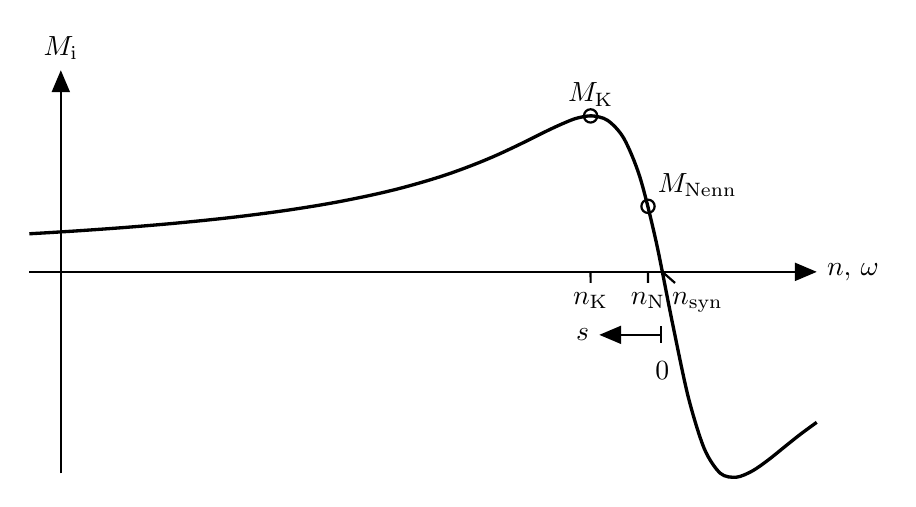
\begin{tikzpicture}[scale=0.8]
\tikzmath{
    \p = 1;
    \ASMms = 3;
    \Us = 100;
    \ASMsigma = 0.067;
    \Xs = 3;
    \Xr = \Xs;
    \Rr = 0.008*\Xr;
    \Rs = 0.01*\Xs;
    \ASMfs = 50;
    \nsyn = 60/2/pi*\ASMfs/\p / (600/12);
    function drehzahl(\s) {
        return (1 - \s)*\ASMfs*60/\p/2/pi;
    };
    \nk = drehzahl(\Rr/\ASMsigma/\Xr) / (600/12);
    \nn = \nk + 0.8*(\nsyn-\nk);
    function schlupf(\n) {
        return 1 - \n*\p/\ASMfs*2*pi/60;  
    };
    function drehmoment(\n) {
        return \ASMms * \p/(2*pi*\ASMfs) * \Us^2 * schlupf(\n)*(1-\ASMsigma)*\Xs*\Xr*\Rr / ((\Rs*\Rr - schlupf(\n)*\ASMsigma*\Xs*\Xr)^2 + (schlupf(\n)*\Rs*\Xr + \Xs*\Rr)^2);
    };
    \Mk = drehmoment(\nk*(600/12))/(250/3.2);
    \Mn = drehmoment(\nn*(600/12))/(250/3.2);
}

    \draw[->, thick, >=triangle 45] (-.5, 0) -- (12, 0) node[right] {$n,\, \omega$};
    \draw[->, thick, >=triangle 45] (0, -3.2) -- (0, 3.2) node[above] {$M_{\mathrm{i}}$};
    
    \node[below right, yshift=-4pt] (nsyn) at (\nsyn, 0) {$n_{\mathrm{syn}}$};
    \node[below, yshift=-4pt] (nk) at (\nk, 0) {$n_{\mathrm{K}}$};
    \node[below, yshift=-4pt] (nn) at (\nn, 0) {$n_{\mathrm{N}}$};
    \node[above] (Mk) at (\nk, \Mk) {$M_{\mathrm{K}}$};
    \node[above right] (Mn) at (\nn, \Mn) {$M_{\mathrm{Nenn}}$};
 
    \draw[thick] (nsyn) -- (\nsyn, 0);
    \draw[thick] (nk) -- (\nk, 0);
    \draw[thick] (nn) -- (\nn, 0);
    \draw[thick] (Mk) -- (\nk, \Mk);
    \draw[thick] (Mn) -- (\nn, \Mn);
    \draw[|->, thick, >=triangle 45] (\nsyn,0) ++(0,-1) node[below, yshift=-6pt] {$0$} -- ++(-1,0) node[left] {$s$}; 
    \draw[mark=*, fill=white, mark options={thick}, only marks, mark size=3pt] plot coordinates {
        (\nk, \Mk) %Kippmoment
        (\nn, \Mn) %Nennmoment
    };
    
    \draw[domain=-.5:12, smooth, variable=\n, very thick, samples=50] plot ({\n}, {drehmoment(\n*(600/12))/(250/3.2)});
\end{tikzpicture}
    \caption{Drehmoment der Asynchronmaschine in Abhängigkeit der Drehzahl $n$. }
    \label{fig:KennlinieASM}
\end{figure}

\subsection{Synchronmaschine}
\label{sec:Synchronmaschine}
Zur Beschreibung der Synchronmaschine sollen im Folgenden das elektrische Ersatzschaltbild der Maschine und die beiden heute gebräuchlichsten Systeme zur elektrischen Erregung betrachtet werden.
\paragraph{Elektrisches Ersatzschaltbild}
Das elektrische Ersatzschaltbild des Schenkelpol-Syn\-chron\-ge\-ne\-ra\-tors zeigt \cref{fig:ESB_SM}. Im Statorkreis der Maschine (siehe \cref{fig:ESB_SM_Stator}) wird durch das Läuferdrehfeld eine ein symmetrisches Drehstromsystem mit der Spannung $\underline{U}_{\mathrm{p}}$ induziert. Wird weiterhin der Statorkreis durch einen Verbraucher geschlossen, so fließt ein Strom $\underline{I}_{\mathrm{s}}$, der neben Verlusten ein Gegenfeld aufbaut, beschrieben durch die fiktive Induktivität $L_{\mathrm{m}}$, welche mit derselben magnetischen Flussänderung $\frac{\mathrm{d} \Phi}{\mathrm{dt}}$ verbunden ist wie die reale Läuferwicklung. Da im Statorkreis nur sinusförmige periodische Zeitverläufe auftreten können diese als komplexe Zeiger dargestellt werden, für den Rotorkreis (siehe \cref{fig:ESB_SM_Rotor}) gilt dies im Allgemeinen nicht.

Aufgrund der Schenkelpole der Maschine ist der Luftspalt nicht konstant und weist eine Achsigkeit auf. Das dreiphasige System des Stators lässt sich als komplexer Raumzeiger darstellen. Als Bezugssystem des Raumzeigers wird ein rotorfestes mitrotierendes Koordinatensystem mit den Achsen $d$ und $q$ so gewählt, dass die $d$-Achse im räumlichen Maximum des Raumzeigers und die $q$-Achse orthogonal dazu liegt. Die beiden Komponenten des Raumzeigers können als Größen einer zweipoligen Ersatzmaschine interpretiert werden, deren Pole in der $d$-Achse und deren Pollücken in der $q$-Achse liegen. Die Angabe der magnetischen Größen des Stators und der elektrischen Größen des Rotors geschieht in Bezug auf dieses Koordinatensystem. Diese Transformation heißt auch \emph{Park-Transformation} oder \emph{d,q-Transformation}.
\begin{figure}
    \centering
    \begin{subfigure}[c]{.66\textwidth}
        \def\THIS{\tikztostart}
\def\normalcoord(#1){coordinate(#1)}
\def\showcoord(#1){coordinate(#1) node[circle, red, draw, inner sep=1pt, pin={[red, overlay, inner sep=0.5pt, font=\tiny, pin distance=0.1cm, pin edge={red, overlay}]45:#1}](){}}
\let\coord=\normalcoord
%\let\coord=\showcoord

\begin{circuitikz}
    \node[ocirc] (Plus) at (0,0) {};
    \node[ocirc] (Minus) at (0,-3) {};
    
    \draw (Plus) to[short, i>^=$\underline{I}_{\mathrm{s}}$] ++(1,0) to[R, R=$R_{\mathrm{s}}$] ++(2,0) to[L, L=$L_{\mathrm{s\sigma}}$] ++(2,0) to[L, L=$L_{\mathrm{md/q}}$] ++(2,0) to[sV, v=$\underline{U}_{\mathrm{p}}$] (\THIS |- Minus) -- (Minus);
    \draw (Plus) to[open, v=$\underline{U}_{\mathrm{s}}$] (Minus);
\end{circuitikz}
        \subcaption{Stator\label{fig:ESB_SM_Stator}}
    \end{subfigure}
    \hskip -3em
    \begin{subfigure}[c]{.33\textwidth}
        \def\THIS{\tikztostart}
\def\normalcoord(#1){coordinate(#1)}
\def\showcoord(#1){coordinate(#1) node[circle, red, draw, inner sep=1pt, pin={[red, overlay, inner sep=0.5pt, font=\tiny, pin distance=0.1cm, pin edge={red, overlay}]45:#1}](){}}
\let\coord=\normalcoord
%\let\coord=\showcoord

\begin{circuitikz}
    \draw (0,0) node[] (Lmr) {} to[L, L=$L_{\mathrm{md/q}}$] ++(2,0) to[short, i<=$i_{\mathrm{r}}(t)$] ++(1,0) node[ocirc] (RPlus) {} to[open, v=$u_{\mathrm{e}}(t)$] ++(0,-2) node[ocirc] (RMinus) {} to[R, R=$R_{\mathrm{rd/q}}$] (Lmr |- RMinus) to[L, L=$L_{\mathrm{r\sigma d/q}}$] (Lmr.center);
    
\end{circuitikz}
        \subcaption{Rotor\label{fig:ESB_SM_Rotor}}
    \end{subfigure}
    \caption{Ersatzschaltbild der Synchronmaschine für $d$- und $q$-Achse des Läufers}
    \label{fig:ESB_SM}
\end{figure}

\paragraph{Erregersystem}
Zur Übertragung der Erregerleistung auf den Rotor des Synchrongenerators werden in der Praxis vor Allem zwei Verfahren eingesetzt:\begin{itemize}
    \item Eine Möglichkeit zur Erregung ist der Einsatz von Schleifringen und Kohlebürsten, die über den Gleitkontakt eine elektrische Verbindung mit einer regelbaren Gleichstromquelle herstellen. Bezeichnet wird diese Methode als \emph{statische Erregung}, da zur Erregung keine rotierenden Maschinen eingesetzt werden. Nachteilig ist, dass der Einsatz der Kohlebürsten und Schleifringe mit Verschleiß und Wartungsarbeiten verbunden ist und unter gewissen Bedingungen es durch den Abrieb der Kohlebürsten zu Bürstenfeuer kommen kann.
    \begin{figure}
        \centering
        \def\THIS{\tikztostart}
\def\normalcoord(#1){coordinate(#1)}
\def\showcoord(#1){coordinate(#1) node[circle, red, draw, inner sep=1pt, pin={[red, overlay, inner sep=0.5pt, font=\tiny, pin distance=0.1cm, pin edge={red, overlay}]45:#1}](){}}
\let\coord=\normalcoord
%\let\coord=\showcoord

\begin{circuitikz}[scale=.5,/tikz/circuitikz/bipoles/length=1cm]
    % Hauptknoten
    \node [circ] (HStar) at (0,0) {};
    \node [circ] (EStar) at (12,-6) {};
    % Stern Haupt
    \draw (HStar) to[L] ++(90:3) node[ocirc] (Ha) {};
    \draw (HStar) to[L] ++(-30:3)  node[ocirc] (Hb) {};
    \draw (HStar) to[L] ++(-150:3) node[ocirc] (Hc) {};
    % Erregung
    \node (Err) at (EStar |- HStar) {};
    \draw (Err) ++(1,1.5) node[ocirc] {} to[short] ++(-1,0) to[L] ++(0,-3) to[short] ++(1,0) node[ocirc] {};
    % Stern Erreger
    \draw (EStar) to[L] ++(60:3) node[] (Ea) {};
    \draw (EStar) to[L] ++(-60:3)  node[] (Eb) {};
    \draw (EStar) to[L] ++(180:3) node[] (Ec) {};
    % Kabel
    \draw (Ea.center) -- (Ec |- Ea) -- ++(0,-2.2) -- ++(-4.5,0) node[circ] (L1) {};
    \draw (Ec.center) -- ++(-3,0) node[circ] (L2) {};
    \draw (Eb.center) -- (Ec |- Eb) -- ++(0,2.2) -- ++(-1.5,0) node[circ] (L3) {};
    % Dioden
    \draw (L1 |- L2) to[D] (L1 |- Ea);
    \draw (L2) to[D] (L2 |- Ea);
    \draw (L3 |- L2) to[D] (L3 |- Ea);
    \draw (L1 |- Eb) to[D] (L1 |- L2);
    \draw (L2 |- Eb) to[D] (L2);
    \draw (L3 |- Eb) to[D] (L3 |- L2);
    % Kabel zu Hauptrotor
    \draw (L3 |- Ea) to[short] (L2 |- Ea) node[circ]{} to[short] (L1 |- Ea) node[circ]{} to[short]  (HStar |- Ea) to[L] (HStar |- Eb) to[short] (L1 |- Eb) node[circ]{} to[short] (L2 |- Eb) node[circ]{} to[short] (L3 |- Eb);
    % Beschriftung
    \node [] (Slabel) at ($(HStar) + (16,0)$) {Ständer};
    \node [] (Rlabel) at (Slabel |- EStar) {Rotor};
    \node [] (Hlabel) at ($(HStar) + (0,-10)$) {Hauptgenerator};
    \node [] (Plabel) at (L2 |- Hlabel) {Diodenrad};
    \node [] (Elabel) at (EStar |- Hlabel) {Erregermaschine};
    % Trennlinien
    \coordinate (hbar) at ($(Hc)!.5!(Ea)$);
    \draw [dashed] (Hc |- hbar) +(-1,0) -- (Slabel |- hbar);
    \coordinate (vbar1) at ($(Hb)!.5!(L1 |- Ea)$);
    \draw [dashed] (vbar1 |- Ha) -- (vbar1 |- Hlabel);
    \coordinate (vbar2) at ($(L3)!.5!(Ec)$);
    \draw [dashed] (vbar2 |- Ha) -- (vbar2 |- Hlabel);
\end{circuitikz}
        \caption{Bürstenloses Erregersystem, eigene Darstellung nach \cite[S. 557]{mullerGrundlagenElektrischerMaschinen2005}}
        \label{fig:burstenloseErregung}
    \end{figure}
    \item Daher findet häufig auch die \emph{bürstenlose Erregung} Verwendung. Sie umgeht den Gleitkontakt durch den Einsatz eines weiteren kleineren Synchrongenerators ausgeführt als \emph{Außenpolmaschine}. Mit dem so erzeugten Drehstrom wird die Erregerwicklung des Hauptgenerators über eine mitrotierende Diodenbrücke gespeist. 
    
    Nachteil dieser Methode ist, dass die Dynamik der Regelstrecke durch die \emph{Erregermaschine} verlangsamt wird und eine Entregung („negative Erregung“) nicht möglich ist. Die Struktur dieses Erregersystems zeigt \cref{fig:burstenloseErregung}. 
\end{itemize}

%----------------------------------------------------
\section{Aus dem Bereich der Modellierung und Simulation}
\label{sec:GrundlagenModellierung}

\subsection{Arten der Modellierung}
\label{subsec:ArtenModellierung}
Grundsätzlich lassen sich alle Konzepte der Modellierung physikalischer Systeme zwei Polen auf einem Spektrum der Einblicktiefe in die Systemstruktur anordnen. So werden Modelle, die nur die Ein- und Ausgangsgrößen in Beziehung zueinander setzen und keine Informationen über die inneren Vorgänge und Zustände des Modells geben, \emph{Blackbox-Modelle} genannt. Modelle hingegen, die vollkommenen Einblick in die Vorgänge und Zustände des modellierten Systems geben, heißen \emph{Whitebox-Modelle}. In der Realität treten diese beiden Extremfälle der Modellierung in den meisten Fällen nicht auf. Viel mehr ist ein Modell häufig aus Anteilen zusammengesetzt, die sich eher einem Blackbox-Modell oder einem Whitebox-Modell zuordnen lassen. Bezeichnet wird diese Unschärfe mit dem Ausdruck \emph{Graybox-Modell}. Typische Beispiele für Modelle, die sich eher als Blackbox-Modell bezeichnet werden können sind \emph{Neuronale Netzwerke}, \emph{Look-Up-Tables} oder Eingangs-Ausgangs-Kennlinien. Modelle wie die \emph{Zustandraumdarstellung}, \emph{Ersatzbilder} o.ä. können hingegen eher als Whitebox-Modell klassifiziert werden. 

Da bei Whitebox-Modellen die Struktur des Systems und seiner Teilsysteme bekannt ist und so die Wiederverwendbarkeit einzelner Teilsysteme ermöglicht wird, sollen für die Modellierung des Frequenzumformers im Folgenden nur Modelle mit überwiegendem Whitebox-Charakter betrachtet werden.

\paragraph{Modellierung mit konzentrierten Elementen} Wird zur Erstellung von Whitebox-Modellen die Realität auf eine endliche Anzahl an Zuständen und Vorgängen reduziert, so handelt es sich um eine Modellierung mit konzentrierten Elementen. Sie steht einer kontinuierlichen Modellierung mit unendlich-dimensionalen Zustandsräumen gegenüber. Letztlich führt jede Modellierung mit konzentrierten Elementen im allgemeinen Fall auf die Simulation eines Systems von Differential- und algebraischen Gleichungen (DAE -- \textbf{D}ifferential \textbf{A}lgebraic \textbf{E}quation). Bekannte Anwendungsbeispiele sind die \emph{Methode der finiten Elemente} oder auch die Modellierung elektrischer, mechanischer und anderer Systeme mit \emph{Ersatzschaltbildern} einfacher konzentrierter Elemente. 

\paragraph{Signal- und Leistungsflussmodelle} Zum Aufstellen der Modelle lassen sich (wenigstens) zwei Abstraktionsebenen zur Abbildung der Realität im Modell unterscheiden, die entsprechend dem jeweiligen Modellierungszweck direkt gewählt oder in einander überführt werden können. Die detailliertesten Modelle sind \emph{Signalflussmodelle} (auch \emph{mathematische Modelle} genannt, da die physikalische Struktur des Systems nicht im Vordergrund steht), das sind direkte Darstellungen der DAE-Systeme, zum Beispiel als \emph{Zustandsraum} mit $n$ Differentialgleichungen erster Ordnung und weiteren Nebenbedingungen oder auch als \emph{Blockschaltbild} (\emph{Signalflussplan}). Charakteristisch für diese Ebene der Modellierung ist, dass die Modelle direkt zur Simulation (meist durch Lösen der algebraischen Gleichungen und Integration der Differentialgleichungen von einem Anfangswert aus) geeignet sind. Die Ursache-Wirkungs-Beziehungen des Systems sind in den beschreibenden Gleichungen bereits festgelegt. Besonders im Vergleich dieser Modelle mit Modellen der höheren Ebene wird dieser Umstand mit \emph{Kausalität} der Wirkrichtung bezeichnet.

Eine höhere Abstraktionsebene als die Signalflussmodellen bilden die \emph{Leistungsflussmodelle} (auch \emph{physikalische Modelle} genannt), 


\subsection{Modellierung elektrischer Maschinen}
\label{subsec:ModellierungElektrischerMaschinen}
%TODO: Beispiele aus Signal- und Leistungsflussmodellierung elektrischer Maschinen beschreiben


\subsection{Übersicht über Simulationsprogramme}
\label{subsec:Simulationsprogramme}
%TODO: Simulationsprogramme vergleichen













\newcommand{\dsize}{width=\textwidth, height=6cm, keepaspectratio}

\chapter{Modellierung}
\label{chap:Modellierung}
%TODO: Einleitung in Modellierung schreiben
Anforderungen:
\begin{itemize}
    \item Universales Modell des Frequenzumformers, zur \begin{itemize}
        \item Untersuchung der Ausgangsspannung bei Lastsprüngen
        \item Untersuchung des Einflusses der Maschinenparameter
        \item Untersuchung des Einflusses der Reglerparameter
    \end{itemize}
    \item Daraus folgt: \begin{itemize}
        \item Korrekte Wiedergabe der übertragenen Leistung
        \item Dynamische Eigenschaften werden so gut wie möglich wiedergegeben
    \end{itemize}
    \item Vernachlässigung folgender Punkte ist möglich: \begin{itemize}
        \item Anfahrverhalten
        \item Temperatureinflüsse
        \item Wirkungsgrad
        \item DC-Abgang der Anlage
    \end{itemize}
    \item Erweiterung und Anpassung des Modells / der Teilmodelle ist möglich
\end{itemize}

\hypertarget{sec:uxfcbersicht---energie--und-informationsfluss}{%
\section{Übersicht - Energie- und Informationsfluss}\label{sec:uxfcbersicht---energie--und-informationsfluss}}

Bevor das Simulationsmodell in Modelica implementiert werden soll, ist es hilfreich zunächst einen Überblick über das Gesamtsystem „rotierender Frequenzumformer“ zu erlangen und die Wirkungseinflüsse der einzelnen Größen zu studieren.

\hypertarget{sec:gesamtsystem}{%
\subsection{Gesamtsystem}\label{sec:gesamtsystem}}

Bei der betrachteten Anlage handelt es sich im Wesentlichen um einen Motor-Generator-Verbund aus einem Asynchronmotor und einem mit einer Synchron-Erregermaschine erregten Synchrongenerator. Das System besteht also aus drei mechanisch gekoppelten elektrischen Maschinen. Der Zusammenhang zwischen den elektrischen Größen am Stator und am Rotor der elektrischen Maschinen sowie die Kopplung mit der rotatorischen Bewegung wird über das Induktionsgesetz durch die Spannung und den Fluss des magnetischen Feldes charakterisiert.

\begin{figure}
    \centering
    \input{Tikz-Bilder/control.tikzstyles}
\begin{tikzpicture}[
    node distance=1cm
    ]
    % Asynchronmaschine
    \node (Netz_in) [bgelement] {Netz-Eingang};
    \node (ASM_Stator) [bgelement, below=of Netz_in] {Stator};
    %\node (ASM_Stator_R) [bgelement, above left=of ASM_Stator] {R};
    %\node (ASM_Stator_L) [bgelement, below left=of ASM_Stator] {L};
    \node (ASM_Luftspalt) [bgelement, below=of ASM_Stator] {Luftspalt};
    \node (ASM_Rotor) [bgelement, below=3cm of ASM_Luftspalt] {Rotor};
    %\node (ASM_Rotor_R) [bgelement, above left=of ASM_Rotor] {R};
    %\node (ASM_Rotor_L) [bgelement, below left=of ASM_Rotor] {L};
    \draw[bonds]
    (Netz_in) edge[flow=$i_{\mathrm{ein}}$, effort=$u_{\mathrm{ein}}$] (ASM_Stator)
    (ASM_Stator) %edge (ASM_Stator_R)
                 %edge (ASM_Stator_L)
                 edge[flow=$\Phi_{\mathrm{s}}$, effort=$V_{\mathrm{m,s}}$] (ASM_Luftspalt)
    (ASM_Luftspalt) edge[flow=$\Phi_{\mathrm{r}}$, effort=$V_{\mathrm{m,r}}$] (ASM_Rotor);
    %(ASM_Rotor) edge (ASM_Rotor_R)
    %            edge (ASM_Rotor_L);
    
    % Mechanik
    \node (Welle) [bgelement, right=1.1cm of ASM_Rotor] {Welle};
    % \node (Reibung) [bgelement, below =of Welle] {Reibung};
    
    \node (Gleichrichter) [bgelement, right=1cm of Welle] {Gleichrichter};
    \draw[bonds] 
        (ASM_Rotor) edge[effort=$M_{\mathrm{Motor}}$, flow=$\omega$] (Welle);
        % (Welle) edge[effort=$M_{\mathrm{Verl.}}$, flow=$\omega$] (Reibung);
    
     % Synchro-Generator
    \node (SG_Luftspalt) [bgelement] at (Gleichrichter|-ASM_Luftspalt.base) {Luftspalt};
    \node (SG_Rotor_Y) [between= Gleichrichter and SG_Luftspalt] {};
    \node (SG_Rotor) [bgelement] at (Gleichrichter|-SG_Rotor_Y) {Rotor};
    %\node (SG_Rotor_R) [bgelement, above right=of SG_Rotor] {R};
    %\node (SG_Rotor_L) [bgelement, below right=of SG_Rotor] {L};
    \node (SG_Stator) [bgelement] at (SG_Luftspalt|-ASM_Stator.base) {Stator};
    %\node (SG_Stator_R) [bgelement, above right=of SG_Stator] {R};
    %\node (SG_Stator_L) [bgelement, above left=of SG_Stator] {L};
    \draw[bonds]
    (Welle) edge[effort=$M_{\mathrm{Gen.}}$, flow=$\omega$] (SG_Rotor)
    (Gleichrichter) edge[effort=$u_{\mathrm{DC}}$, flow=$i_{\mathrm{DC}}$] (SG_Rotor)
    (SG_Rotor) edge[flow=$\Phi_{\mathrm{r}}$, effort=$V_{\mathrm{m,r}}$] (SG_Luftspalt)
               %edge (SG_Rotor_R)
               %edge (SG_Rotor_L)
    (SG_Luftspalt) edge[flow=$\Phi_{\mathrm{s}}$, effort=$V_{\mathrm{m,s}}$] (SG_Stator);
    %(SG_Stator) edge (SG_Stator_R)
    %            edge (SG_Stator_L);
    
    % Erregermaschine
    \node (EM_Rotor) [bgelement, below=of Gleichrichter] {Rotor};
    %\node (EM_Rotor_R) [bgelement, below left=of EM_Rotor] {R};
    %\node (EM_Rotor_L) [bgelement, below right=of EM_Rotor] {L};
    \node (EM_Luftspalt) [bgelement, right=of EM_Rotor] {Luftspalt};
    \node (EM_Stator) [bgelement, right=of EM_Luftspalt] {Stator};
    %\node (EM_Stator_R) [bgelement, below left=of EM_Stator] {R};
    %\node (EM_Stator_L) [bgelement, below right=of EM_Stator] {L};
    
    \draw[bonds]
    (Welle) edge[effort=$M_{\mathrm{Err.}}$, flow=$\omega$] (EM_Rotor)
    (EM_Rotor) edge[effort=$u_{\mathrm{AC}}$, flow=$i_{\mathrm{AC}}$] (Gleichrichter)
               %edge (EM_Rotor_L)
               %edge (EM_Rotor_R)
    (EM_Luftspalt) edge[flow=$\Phi_{\mathrm{r}}$, effort=$V_{\mathrm{m,r}}$] (EM_Rotor)
    (EM_Stator) edge[flow=$\Phi_{\mathrm{s}}$, effort=$V_{\mathrm{m,s}}$] (EM_Luftspalt);
                %edge (EM_Stator_R)
                %edge (EM_Stator_L);
    
    % Last
    \node (Last) [bgelement] at (EM_Stator|-SG_Stator) {Last};
    \draw[bonds] (SG_Stator) edge[flow=$i_{\mathrm{aus}}$, effort=$u_{\mathrm{aus}}$] (Last);
    
    % Regler
    \node (Summe) [sum, below=of Last] {};
    \node (Sollspannung) [input, right=of Summe, label=$U_{\mathrm{aus,soll}}$] {};
    \node (Regler) [block, label={right:}] at ($(Summe)!1/3!(EM_Stator)$) {PID};
    \node (PWM) [pulse, label={right:PWM}] at ($(Summe)!2/3!(EM_Stator)$) {};
    \draw[signal] (Last) -- node[left] (U_Regler_in) {$U_{\mathrm{aus,ist}}$} (Summe);
    \draw[signal] (Sollspannung) -- node[near end,below]{\small $-$} (Summe);
    \draw[signal] (Summe) -- (Regler);
    \draw[signal] (Regler) -- (PWM);
    \draw[bonds] (PWM) ++(0,-.6) edge[effort=$u_{\mathrm{err}}$, flow=$i_{\mathrm{err}}$] (EM_Stator);
    
    %Beschriftung
    \node [below=.3cm of EM_Luftspalt] {Erregermaschine};
    \node [above=.3cm of SG_Stator] {Synchrongenerator};
    \node [below=.3cm of ASM_Rotor] {Asynchronmaschine};
    \node [right=.3cm of Regler, align=center] {Regler-\\ board};
    \begin{pgfonlayer}{background}
    \filldraw [line width=4mm,join=round,black!5]
      (Netz_in.west|-Netz_in.north)  rectangle (Netz_in.east|-ASM_Rotor.south)
      (SG_Luftspalt.west|-SG_Stator.north) rectangle (SG_Luftspalt.east|-SG_Rotor.south)
      ($(EM_Rotor.west|-EM_Rotor.north) + (0,.1)$) rectangle ($(EM_Stator.east|-EM_Stator.south) + (0,-.1)$);
      %($(U_Regler_in.west) + (0,.2)$) rectangle ($(Sollspannung.east|-PWM.east) + (.4,-.4)$);
  \end{pgfonlayer}
\end{tikzpicture}
    \caption{Energie- und Informationsfluss des rotierenden Frequenzumformers}
    \label{fig:Wirkungsgraph}
\end{figure}

In Anlehnung an die Bondgraphen-Methode zeigt der ``Wort-Bondgraph''(oder ``Wortgraph'', vgl. \cite[S.~10]{roddeckBondgraphenModellbildungUnd2019}) in \cref{fig:Wirkungsgraph} den Energie- und Informationsfluss im Frequenzumformer. Die Halbpfeile (\bond) repräsentieren den Energiefluss (die übertragene Leistung) der zusammenhängenden \emph{Fluss-} (\emph{Flow}) und \emph{Potential}größen (\emph{Effort}). Nach Konvention werden die Potentialgrößen oberhalb und die Flussgrößen unterhalb der Halbpfeils aufgetragen. Alternativ kann auch die Flussgröße direkt an einem Knoten notiert werden, wenn die Größe für alle verbundenen Kanten konstant ist. 

Im Gegensatz zu den formalen Bondgraphen können die Knoten des Wortgraphen mehrere Größen und Verbindungen, die zum Aufstellen des Zustandsraummodells nötig wären, unter einem Oberbegriff zusammenfassen und vereinfachen (\emph{Objektorientierung}). Ist eine solche detaillierte Darstellung gesucht, können die einzelnen Oberbegriffe jeweils durch ihre korrespondierenden Bondgraph-Darstellungen ersetzt werden. Bondgraphen für die einzelnen elektrischen Maschinen können beispielsweise \cite[S.~269~ff.]{borutzkyBondGraphModelling2011} entnommen werden.

Ursache für den in \cref{fig:Wirkungsgraph} dargestellten Energiefluss ist der Vorgabe der Spannung am Netz-Eingang. Sie bewirkt einen Stromfluss im Stator, der einerseits zur Speicherung (Streuinduktivität) und Abgabe (ohm'sche Verluste) elektrischer Energie in den Statorwindungen führt und andererseits zur Wandlung elektrischer Energie in magnetische führt. Diese Energie wird über den Luftspalt (der wie ein Transformator das Verhältnis der magnetischen Spannung zum Fluss wandelt auf den Rotor übertragen (Beachte den Bezug auf Stator- (s) bzw. Rotorseite (s).). Im Rotor wird eine Spannung induziert, die einen Stromfluss zur Folge hat. Über die Lorentzkraft folgt die Wandlung in kinetische (rotatorische) Energie.

Während die Winkelgeschwindigkeit der Welle für angrenzenden Baugruppen gleich ist, teilt sich das Motormoment auf. Ein Teil der Energie wird über die Massenträgheit in der Welle gespeichert und ein Teil verlässt das System durch Reibungseffekte (Lagerreibung, Luftwiderstand, \ldots). Der größte Teil wird jedoch an den Synchrongenerator und die Erregermaschine übertragen.

Die Hauptaufgabe der Erregermaschine ist es, die Spannung am Ausgang des Reglersystems berührunglos auf den Rotor des Synchrogenerators zu übertragen. Dies geschieht durch Wandlung der elektrischen Energie und Übertragung über den Luftspalt der Maschine. Gekoppelt sind Generator und Erregermaschine über den mitrotierenden Gleichrichter. Der Synchrongenerator wandelt die eingebrachte mechanische Energie und die Erregung über den Luftspalt in elektrische Energie.

Zusätzlich zu dem Energiefluss ist in \cref{fig:Wirkungsgraph} auch der Informationsfluss angedeutet: Am Ausgang des Umformers wird der Spannungsabfall über der Last gemessen und die Differenz zum Sollwert in den Regler zurückgeführt. Der PID-Spannungsregler ist hier zusammengefasst dargestellt. Ein ausführliches Blockschaltbild des Reglers zeigt \cref{fig:Blockschaltbild_Regler}. Aus der vom Regler berechneten Stellgröße wird über Puls-Weiten-Modulation eines Steuertrafos die Statorspannung der Erregermaschine erzeugt.

\hypertarget{sec:pid-spannungsregler}{%
\subsection{PID-Spannungsregler}\label{sec:pid-spannungsregler}}

Als Spannungsregler wird von Piller in dem Frequenzumformer ein PID-Regler mit \emph{variabler Verstärkung} eingesetzt. Die variable Verstärkung dient zum Erreichen eines besseren Einschwingverhaltens bei großen Regelabweichungen (vgl. \cite{DigitalerSpannungsreglerSoftwaredokumentation}). \cref{fig:Blockschaltbild_Regler} zeigt das Blockschaltbild des Reglers. Der PID-Regler ist in Parallelstruktur ausgeführt; an den Ausgängen der Regelglieder und am Gesamtausgang werden die Stellgrößen begrenzt. 

\begin{figure}
    \centering
    \input{Tikz-Bilder/control.tikzstyles}
\begin{tikzpicture}[node distance=1.5cm]
		% I-Regulator
		\node [integral, label={below:I-Regler}] (I-Reg) at (0,0) {};
		\node [limiter] (I-Lim) [right of=I-Reg] {};
		\node [sum] (sum) [right of=I-Lim] {};
		\node [limiter] (All-Lim) [right of=sum] {};
		\node [pulse, label={[align=center] below:Pulsweiten-\\Modulator}] (PulseModulator) [right of=All-Lim] {};
		% D-Regulator
		\node [differential, label={below:D-Regler}] (D-Reg) [below of=I-Reg] {};
		\node [limiter] (D-Lim) [right of=D-Reg] {};
		% P-Regulator
		\node [proportional, label={below:P-Regler}] (P-Reg) [above of=I-Reg] {};
		\node [limiter] (P-Lim) [right of=P-Reg] {};
		% PP-Regulator
		\node [proportional, label={above:Gain-Regler}] (PP-Reg) [above of=P-Reg] {};
		\node [limiter] (PP-Lim) [right of=PP-Reg] {};
        \node (PP_h) at ($ (sum|-PP-Lim) + (0,-.6) $) {};
        % Input and Knots
		\node [splitter] (knot1) [left of=I-Reg] {};
		\node [splitter] (knot2) [left of=P-Reg] {};
		\node [input] (input) [left of=knot1] {};
        \node (output) [node distance=1.5cm, right of=PulseModulator]{};
        
        %% Edges
        \draw [signal] (input) -- (knot1) -- (I-Reg);
        % I-Regulator
        \draw [signal] (I-Reg) -- (I-Lim);
        \draw [signal] (I-Lim) -- (sum) node [xshift=-0.6cm, above] {\footnotesize$+$};
        % D-Regulator
		\draw [signal] (knot1) |- (D-Reg);
		\draw [signal] (D-Reg) -- (D-Lim);
		\draw [signal] (D-Lim) -| (sum) node [yshift=-0.6cm, left] {\footnotesize$+$};
		% P-Regulator
		\draw [signal] (knot1) |- (P-Reg);
		\draw [signal] (P-Reg) -- (P-Lim);
		\draw [signal] (P-Lim) -| (sum) node [yshift=0.6cm, right] {\footnotesize$+$};
		% PP-Regulator
		\draw [signal] (knot1) |- (PP-Reg);
		\draw [signal] (PP-Reg) -- (PP-Lim);
		\draw [signal] (PP-Lim) -| (PP_h.center) -| (P-Reg);
		% Output
		\draw [signal] (sum) -- (All-Lim);
		\draw [signal] (All-Lim) -- (PulseModulator);
		\draw [signal] (PulseModulator) -- (output);
\end{tikzpicture}
    \caption{Blockschaltbild des Reglers}
    \label{fig:Blockschaltbild_Regler}
\end{figure}

Implementiert ist der PID-Regler als digitaler Regler auf einem Mikrocontroller. Dabei sind einige Punkte zu beachten:
\begin{itemize}
    \item {Die Algorithmen für die Regelglieder arbeiten zeitdiskret. Zur Ableitung der Algorithmen muss die Abtastung mit einem ZOH-Glied beim Anwenden der $\mathcal{Z}$-Transformation berücksichtigt werden, siehe \cref{par:ZeitdiskreterRegler}.}
    \item {Die Abtastung der Ausgangsspannung erfolgt nach \cite{DigitalerSpannungsreglerSoftwaredokumentation} bei dem hier betrachteten Spannungsregler mit 32 Messwerten in 5 Taktzyklen, wobei sich die Taktfrequenz nach der Frequenz der Ausgangsspannung richtet. Die Abtastrate für die Spannungsmessung beträgt also
    \begin{align}
        T_{\mathrm{mess}}^*&= \frac{5}{32}\cdot T_{\mathrm{Spannung}} = 0,000390625\,\mathrm s. \\
        \text{mit} \quad
        T_{\mathrm{Spannung}}&= \frac{1}{400\,\mathrm{Hz}}=0,0025\,\mathrm s
    \end{align}
    Weiterhin gibt \cite{DigitalerSpannungsreglerSoftwaredokumentation} an, dass bei einer Spannungsfrequenz von \(f=400\,\mathrm{Hz}\) der Regelalgorithmus nur alle zwei Messzyklen neu berechnet wird. Die Periodendauer des zeitdiskreten Reglers beträgt also
    \begin{align}
        T_{mess}&=2\cdot T_{mess}^*= 0,00078125\,\mathrm s.
    \end{align} }
    \item {Die Digitalisierung der Spannungsmessung bedeutet eine Quantisierung der Werte. Die gemessenen Werte werden Reglerintern auf \(2^{16}\) ganzzahlige vorzeichenbehaftete Werte (\emph{``16 bit signend integer''}) abgebildet, also auf das Intervall \([-32768,32767]\). Um den Zusammenhang zwischen der realen Spannung und der internen Darstellung herzustellen, müssen Umrechnungsfaktoren angegeben werden.}
\end{itemize}


\hypertarget{sec:umsetzung}{%
\section{Umsetzung}\label{sec:umsetzung}}
%TODO: Referenzen überarbeiten
Die im Folgenden beschriebene Modellierung des Frequenzumformers erfolgt auf Basis der \modclass{Modelica\ Standard\ Library\ v3.2.3} (MSL, siehe \cite[]{modelicaassociationModelicaStandardLibrary2020}). So weit nicht weiter angegeben sind alle im Folgenden angegebenen Bibliotheken und Klassen abgeleitete Klassen der MSL. Für das entwickelte Modell und benötigte Hilfsklassen wird eine eigenständige Bibliothek \modclass{Frequenzumformer} angelegt. Alle Klassen, die dieser Bibliothek angehören werden mit \modclass{Frequenzumformer.Klasse} bezeichnet. Die vollständige Bezeichnung der abgeleiteten Klassen zeigt die Hierarchie der jeweiligen Bibliothek. Beginnend bei dem Bibliotheksnamen wird jedes untergeordnete Objekt mit einem Punkt abgetrennt angefügt, z.B. \modclass{Modelica.Bibliothek.Unterobjekt}.

Für den Asynchronmotor und den Synchrongenerator werden die Modelle \modclass{AIM\_­Squir­rel­Cage} und \modclass{SM\_ElectricalExcited} aus der Bibliothek \modclass{Mag\-netic.\-Funda\-men\-tal\-Wave} der MSL verwendet. Die Herleitung dieser Modelle ist umfangreich in \cite[]{kralModelicaObjektorientierteModellbildung2019} beschrieben und soll hier nur kurz zusammengefasst werden. Verwendet werden die jeweiligen transienten elektrischen Komponenten und Maschinen, da nur mit diesen Einschwingvorgänge beobachtet werden können. Die quasistationären Modelle (Klassen in den Paketen \modclass{Electrical.QuasiStationary} und \modclass{Magnetic.QuasiStatic}) verwenden zur Berechnung der elektrischen und magnetischen Größen komplexe Zeiger. Diese sind nicht geeignet zur Untersuchung von Einschwingvorgängen, da die Zeiger aus der Fouriertransformation periodischer eingeschwungener Größen hergeleitet werden.


Nach \cite[S. 149]{kralModelicaObjektorientierteModellbildung2019} werden für die betrachteten Maschinen in der MSL folgende Voraussetzungen und Vereinfachungen getroffen:
\begin{itemize}
\item
  Die Wicklungen sind vollständig symmetrisch ausgeführt.
\item
  Oberwellen der magnetischen Größen im Luftspalt werden vernachlässigt.
\item
  Sättigungseffekte werden vernachlässigt.
\end{itemize}

\hypertarget{sec:asynchronmotor-mit-kurzschlussluxe4ufer}{%
\subsection{Asynchronmotor mit Kurzschlussläufer}
\label{sec:asynchronmotor-mit-kurzschlussluxe4ufer}}

Da die betrachteten Drehfeldmaschinen in vielen Bereichen gleich oder zumindest ähnlich aufgebaut sind, legt \cite{kralModelicaObjektorientierteModellbildung2019} den Asynchron- und Synchronmaschinen der MSL ein \emph{partielles Modelica-Modell} (Modell, das mit dem Modifizierer \modclass{partial} versehen ist. Das Modell muss nicht die gleiche Anzahl von Gleichungen und Unbekannten haben. Es bietet die Möglichkeit Strukturen des Modells bei der Vererbung zu verändern (\modclass{replace}). Ein solches Modell kann nicht allein simuliert werden.) für Drehfeldmaschinen zugrunde (\modclass{FundamentalWave.­In­ter­fa­ces.­Par­tial­Ba­sic­In­duc­tion­Ma­chine}). Das unterstützt den objektorientierten Modellierungsansatz, sodass diese Grundstruktur nicht für jede elektrische Maschine neu aufgestellt werden muss.


\hypertarget{sec:partielles-modell-der-drehfeldmaschine}{%
\subsubsection{Partielles Modell der Drehfeldmaschine}\label{sec:partielles-modell-der-drehfeldmaschine}}

Das partielle Modell der Drehfeldmaschine (siehe \cref{fig:partiellDrehfeldmaschinen}) modelliert die Energieübertragung vom elektrischen Netzanschluss des Stators über den Luftspalt auf den Rotor, wie sie schon in \cref{fig:Wirkungsgraph} betrachtet wurde. Die Ausgestaltung des Rotormodells und der mögliche Anschluss elektrischer Klemmen an den Rotor (z.B. über Schleifringe) ist dann Teil der Spezialisierung des Modells für die einzelnen elektrischen Maschinen. Neben der Stator-Rotor-Kopplung bietet das partielle Modell auch einen Sammelpunkt für Wärmeenergie aller Teilkomponenten, eine mechanische Trägheitskomponente für die Trägheit des Rotors der Maschine verbunden mit einem Lagerreibungsmodell und einem optionalen mechanischen Anschluss zur Abstützung des Stators.

\begin{figure}
\centering
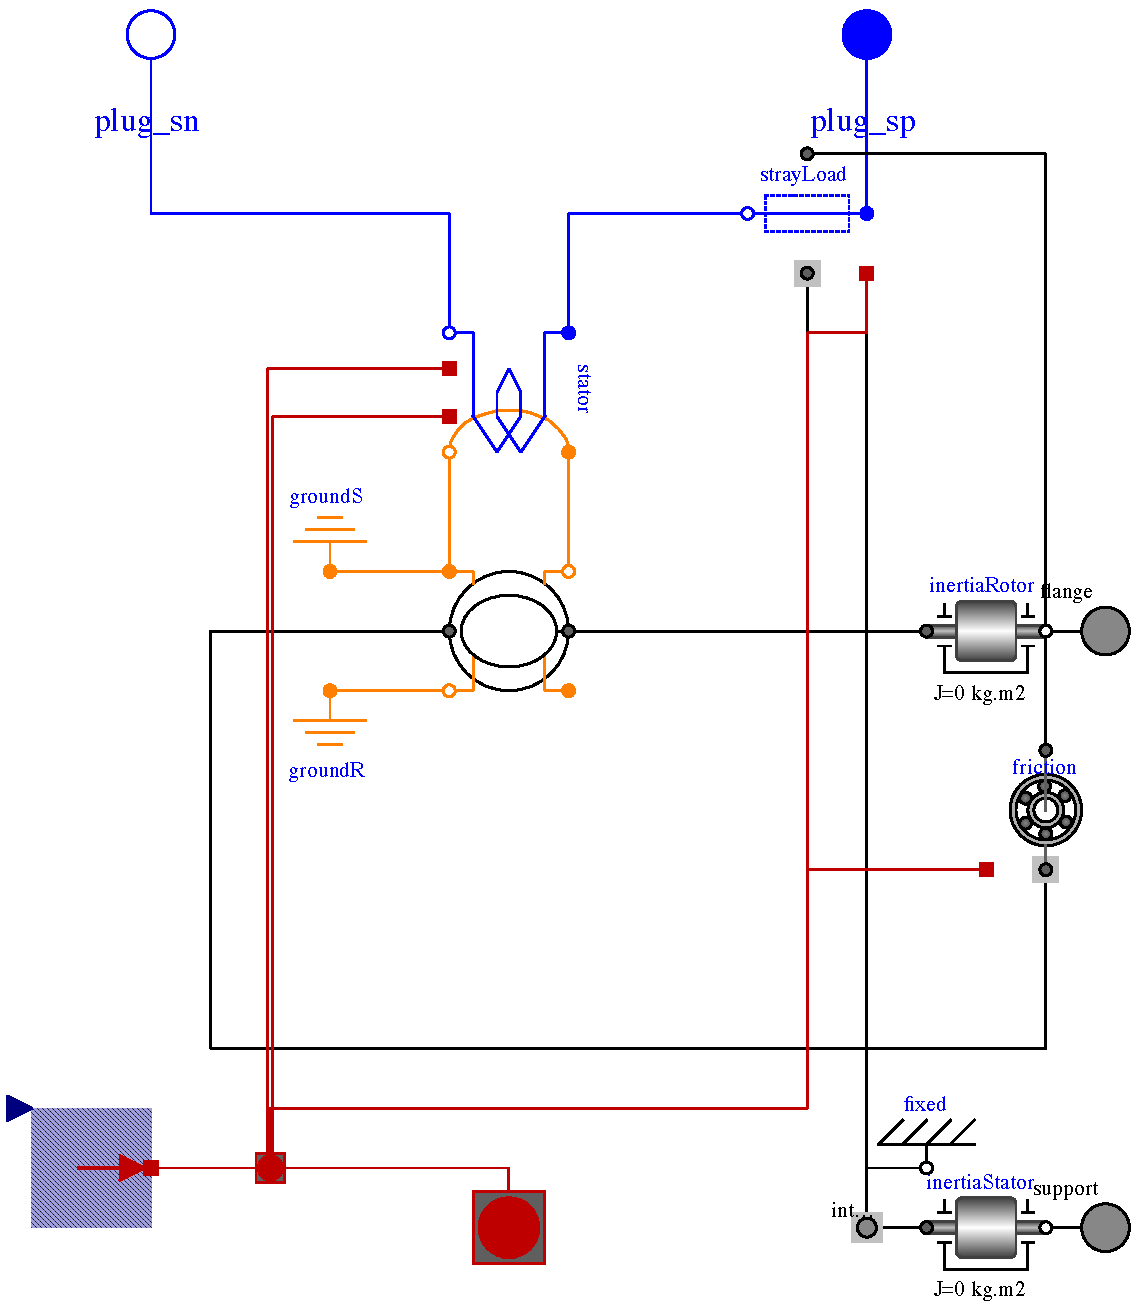
\includegraphics[height=6cm]{Bilder/PartialBasicInductionMachine.pdf}
\caption{Partielles Modell der Drehfeldmaschine \modclass{Fun­da­men­tal­Wave.­In­ter­fa­ces.­PartialBasicInductionMachine} der MSL v3.2.3}
\label{fig:partiellDrehfeldmaschinen}
\end{figure}

Die Energiewandlung im Stator (siehe \cref{fig:MultiPhasenWindung}) geschieht über das Windungsmodell \modclass{Fun­da­men­tal­Wave.­Ba­sic­Ma­chines.­Com­po­nents.­Sym­me­tric­Mu­lti­Phase­Win­ding}, welches neben der elektro-magnetischen Kopplung auch ohmsche Verluste sowie Streu- und Wirbelstromverluste des Magnetfelds berücksichtigt. Außerdem berücksichtigt das Modell  bei ungeradzahligen mehrphasigen Systemen noch die Nullinduktivität. Das wird jedoch nur benötigt, wenn die Windung unsymmetrisch belastet wird (\cite[S. 193]{kralModelicaObjektorientierteModellbildung2019}), was in der hier betrachteten Anwendung nicht auftritt.

% \begin{figure}
% \centering
% 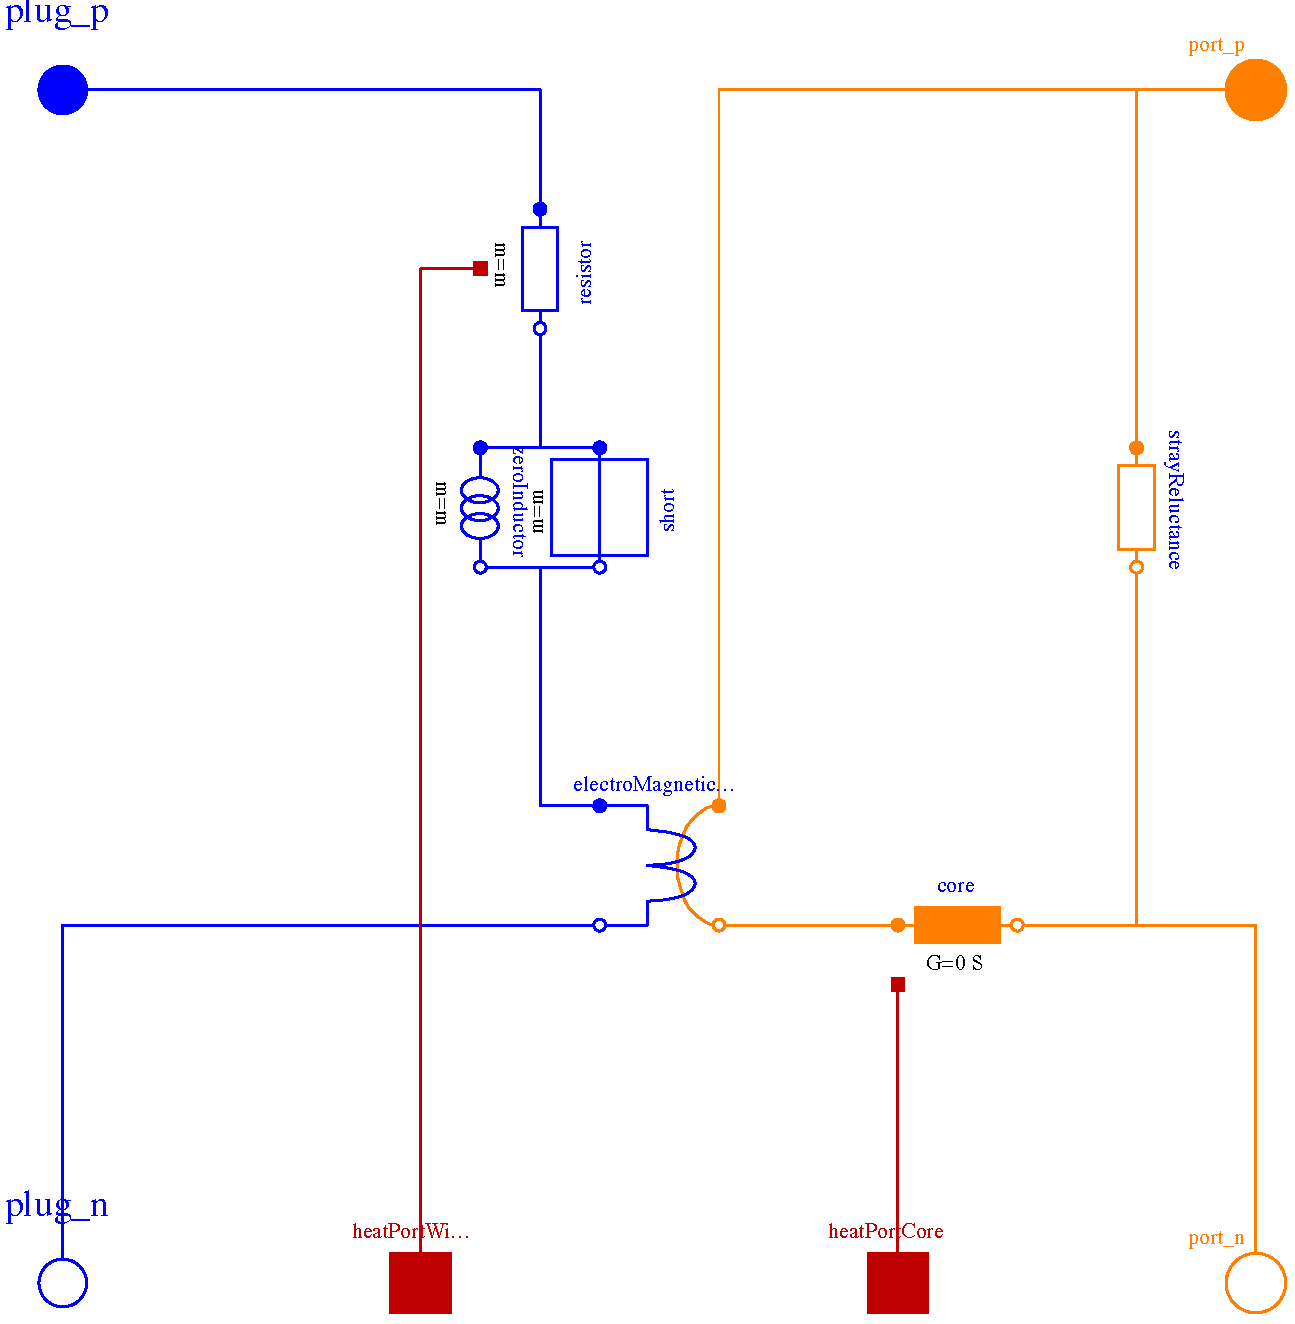
\includegraphics[height=6cm]{Bilder/SymmetricMultiPhaseWinding.pdf}
% \caption{Windungsmodell \modclass{FundamentalWave.Basic­Ma­chines.­Com­po­nents.­Sym­me­tric­Mu­lti­Phase­Win­ding}
% der MSL v3.2.3}
% \label{fig:MultiPhasenWindung}
% \end{figure}

Über das Luftspaltmodell (\modclass{FundamentalWave.BasicMachines.­Com­po­nents.­Ro­tor­Sa­li­en­cy­Air­Gap}) wird der Abfall der magnetischen Spannung über dem magnetischen Widerstand des Luftspalts sowie das auf den Rotor wirkende Drehmoment modelliert. Um die magnetischen Größen des Stators und des Rotors in Beziehung zueinander zu setzen ist eine Koordiantentransformation der Statorgrößen in das körperfeste Bezugssystem des Rotors implementiert (\emph{d,q-System}).

\hypertarget{sec:modell-ASM}{%
\subsubsection{Modell}\label{sec:modell-ASM}}

Das vollständige Modell der Asynchronmaschine mit Kurzschlussläufer (\modclass{Fun­da­men­tal­Wave.­Ba­sic­Ma­chines.­A­syn­chro­nous­In­duc­tion­Ma­chines.­AIM­\_­Squir­rel­Cage}) zeigt \cref{fig:ASM_vollstaendig}. Es ergibt sich aus dem partiellen Modell durch Hinzufügen des kurzgeschlossenen Käfigmodells (\modclass{Fun­da­men­tal­Wave.Ba­sic­Ma­chines.­Com­po­nents.­Sym­me­tric­Mul­ti­Phase­Cage­Win­ding}).

Da die Anzahl \(N_{\mathrm{R}}\) der Rotorstäbe eines Käfigs häufig viel größer ist als die Anzahl (m) der Phasen des Systems, ist es numerisch einfacher für den Käfig eine (m)-phasige kurzgeschlossene Windung als Ersatzmodell zu verwenden, welche die gleiche effektive Windungszahl wie die Statorwicklung aufweist. (\cite[S. 194]{kralModelicaObjektorientierteModellbildung2019})

\begin{figure}
\centering
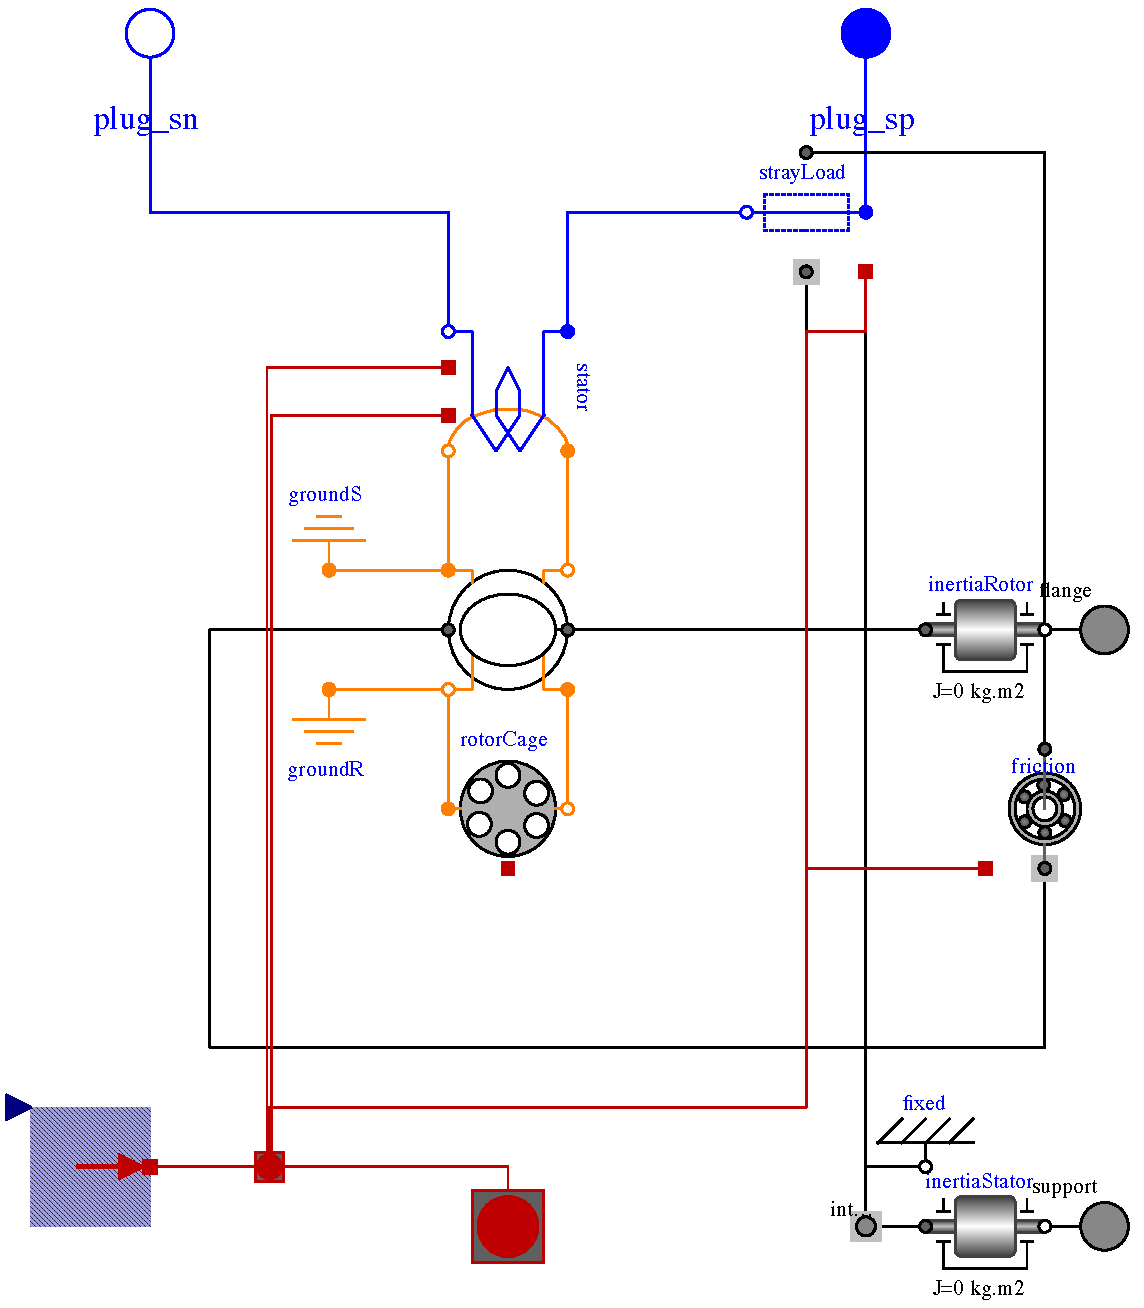
\includegraphics[width=.45\textwidth]{Bilder/AIM_SquirrelCage.pdf}
\caption{Vollständiges Modell der Asynchronmaschine mit Kurzschlussläufer (\modclass{Fun­da­men­tal­Wave.­Ba­sic­Ma­chines.­A­syn­chro­nous­In­duc­tion­Ma­chines.­AIM\_­Squir­rel­Cage}) der MSL v3.2.3}
\label{fig:ASM_vollstaendig}
\end{figure}

% \begin{figure}
% \centering
% 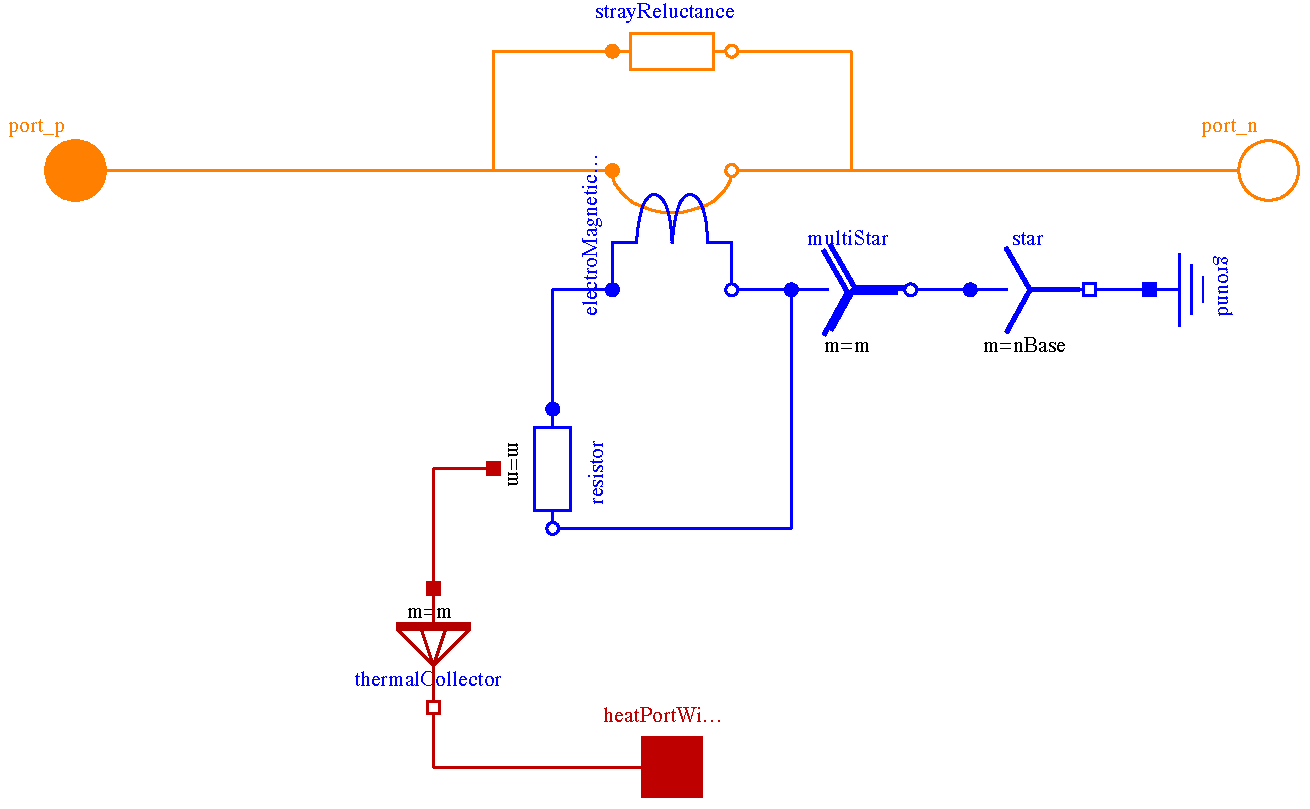
\includegraphics[]{Bilder/SymmetricMultiPhaseCageWinding.pdf}
% \caption{M-phasiges Käfig-Ersatzmodell (\modclass{Fun­da­men­tal­Wave.­Com­po­nents.­Sym­metric­Mul­ti­Phase­Cage­Win­ding}) der MSL v3.2.3}
% \label{fig:MPhasigerKaefig}
% \end{figure}

\hypertarget{sec:parametrierung-ASM}{%
\subsubsection{Parametrierung}\label{sec:parametrierung-ASM}}

Zur Parametrierung der Maschine müssen drei Arten von Größen angegeben werden: elektrische, mechanische und thermische Größen. Da bei Adaptieren des Fre­quenz­um­for­mer-Modells auf andere Maschinengrößen vorrangig die elektrischen und mechanischen Größen angepasst werden müssen, werden diese Werte in einem eigenen Record-Modell (\modclass{Frequenzumformer.Maschinenparameter.AIM\_­Squir­rel­Cage­Da­ta}, siehe \cref{lst:RecordASMData}) zusammengefasst. Das ermöglicht auch die Umrechnung der im Datenblatt der Maschine angegebenen Reaktanzen in die für die Simulation benötigten Induktivitäten.

Die thermischen Größen (Betriebspunkts- und Referenztemperaturen von Stator und Rotor, Temperaturabhängigkeit der Widerstände) werden auf (\unit[20]{°C}) Umgebungstemperatur eingestellt, wobei die Temperaturabhängigkeit der Widerstände vernachlässigt werden soll.

Wie schon oben erwähnt, verwendet das Modell der Asynchronmaschine nach außen hin zur Parametrierung der Wicklungen Stator- und Rotorinduktivitäten, sowie die effektive Statorwindungszahl. Die Induktivitäten sind die auch im T-Ersatzschaltbild der Maschine (vgl. \cref{fig:ESB_ASM}) angegeben Größen: Hauptfeldinduktivität (\(L_m\)), Stator-Streuinduktivität (\(L_{s\sigma}\)) und Rotor-Streuinduktivität (\(L_{r\sigma}\)). Im Datenblatt der Maschine sind die Reaktanzen \(X_0, X_1, X_2\) angegeben. Die zugehörigen Induktivitäten ergeben sich mit der Netzfrequenz \(f_{Netz}=\unit[50]{\mathrm{Hz}}\) nach
\begin{align}
    L_m &= \frac{X_0}{2\pi f_{Netz}} \\
    L_{s,\sigma} &= \frac{X_1}{2\pi f_{Netz}} \\
    L_{r,\sigma} &= \frac{X_2}{2\pi f_{Netz}}.
\end{align}
Für die effektive Windungszahl (\modclass{effectiveStatorTurns}) gibt \cite[S. 217]{kralModelicaObjektorientierteModellbildung2019}
\begin{equation}
    N_{\mathrm{eff. s}} = \hat{N}\cdot\xi_{\mathrm{c}}\cdot\xi_{\mathrm{z}}\label{eq:effStatorTurns},
\end{equation}
an, mit der \emph{Statorwindungszahl} \(\hat{N}\), dem \emph{Sehnungsfaktor} \(\xi _{\mathrm{c}}\) und dem \emph{Zonenfaktor} \(\xi _{\mathrm{z}}\). Ebenda angegeben sind die \cref{eq:xic,eq:xiz} für die beiden Faktoren \(\xi _{\mathrm{c}}\) und \(\xi_{\mathrm{z}}\) (\cite[S. 165, S. 217]{kralModelicaObjektorientierteModellbildung2019}).
\begin{align}
    \xi _{\mathrm{c}} &= \sin(\frac{\Delta\gamma _{\mathrm{c}}}{2}) \label{eq:xic}\\
    \xi _{\mathrm{z}} &= \frac{\sin(\frac{\pi}{6})}{q\sin(\frac{\pi}{6q})}\label{eq:xiz}
\end{align}
Die \emph{Spulenweite} \(\Delta\gamma _{\mathrm{c}}\) ist gemäß
\begin{equation}
    \Delta\gamma _{\mathrm{c}} = 2\pi\cdot\frac{y _{\mathrm{Q}}}{S'}
\end{equation}
das Verhältnis des \emph{Nutschritts} (\(y_Q\)) zur Anzahl der \emph{Nuten je Polpaar} (\(S'=\sfrac{Q}{2p}\)) multipliziert mit \(2\pi\) (\cite[S. 168, S. 161]{kralModelicaObjektorientierteModellbildung2019}), vgl. \cite[S. 76, S. 119]{binderElektrischeMaschinenUnd2012}). Ebenso ist die \emph{Lochzahl} (\(q\)) zur Berechnung des Zonenfaktors das Verhältnis der Anzahl der Nuten zur Anzahl der Stränge und Pole (vgl. \cite[S. 151]{kralModelicaObjektorientierteModellbildung2019})
\begin{equation}
    q = \frac{Q}{2pm}\label{eq:Lochzahl}.
\end{equation}
Damit ist die Statorwindung der Asynchronmaschine vollständig parametriert. Die Wicklungsdaten und die daraus nach \crefrange{eq:effStatorTurns}{eq:Lochzahl} berechneten Werte listet \cref{XXX} auf. Alle weiteren Größen zur Beschreibung der Asynchromaschine können direkt aus dem Datenblatt entnommen und sind ebenfalls in \cref{XXX} angegeben. 

Dabei ist für das Trägheitsmoment \(J_{\mathrm{r}}=0\) eingetragen, da aus der Auslegung des Frequenzumformers nur ein kombiniertes Trägheitsmoment der Welle mit den Rotoren aller drei Maschinen und dem Lüfter bekannt ist. Da die die Modellierung der Welle starr (d.h. ohne Berücksichtigung der Elastizität oder der inneren Dämpfung der Welle) geschieht, kann dieses kombinierte Trägheitsmoment im Trägheitsmoment des Lüftermodells zusammengefasst werden.

\subsection{Synchrongenerator mit Dämpferkäfig}\label{sec:synchrongenerator}

Das Modell des Synchrongenerators basiert wie auch das der Asynchronmaschine auf dem oben schon dargestellten partiellen Drehfeldmaschinenmodell. Es fügt dem partiellen Modell ein einphasiges elektro-magnetisches Kopplungsmodell und ein Bürstenmodell für die elektrische Erregung hinzu und bietet einen optionalen Dämpferkäfig, ähnlich zu dem Kurzschlussläufer der Asynchronmaschine.

\hypertarget{sec:Modell-SG}{%
\subsubsection{Modell}\label{sec:Modell-SG}}

\cref{XXX} zeigt das vollständige Modell des elektrisch erregten Synchrongenerators mit Dämpferkäfig. Die Verwendung des Dämpferkäfigs wird über den Parameter \modclass{useDamperCage} eingestellt. Wird dieser Parameter auf \modclass{false} gesetzt, wird das Modell mit dem Verbindungsmodell \modclass{short} anstelle des Dämpferkäfigs initialisiert. 
\begin{figure}
    \centering
    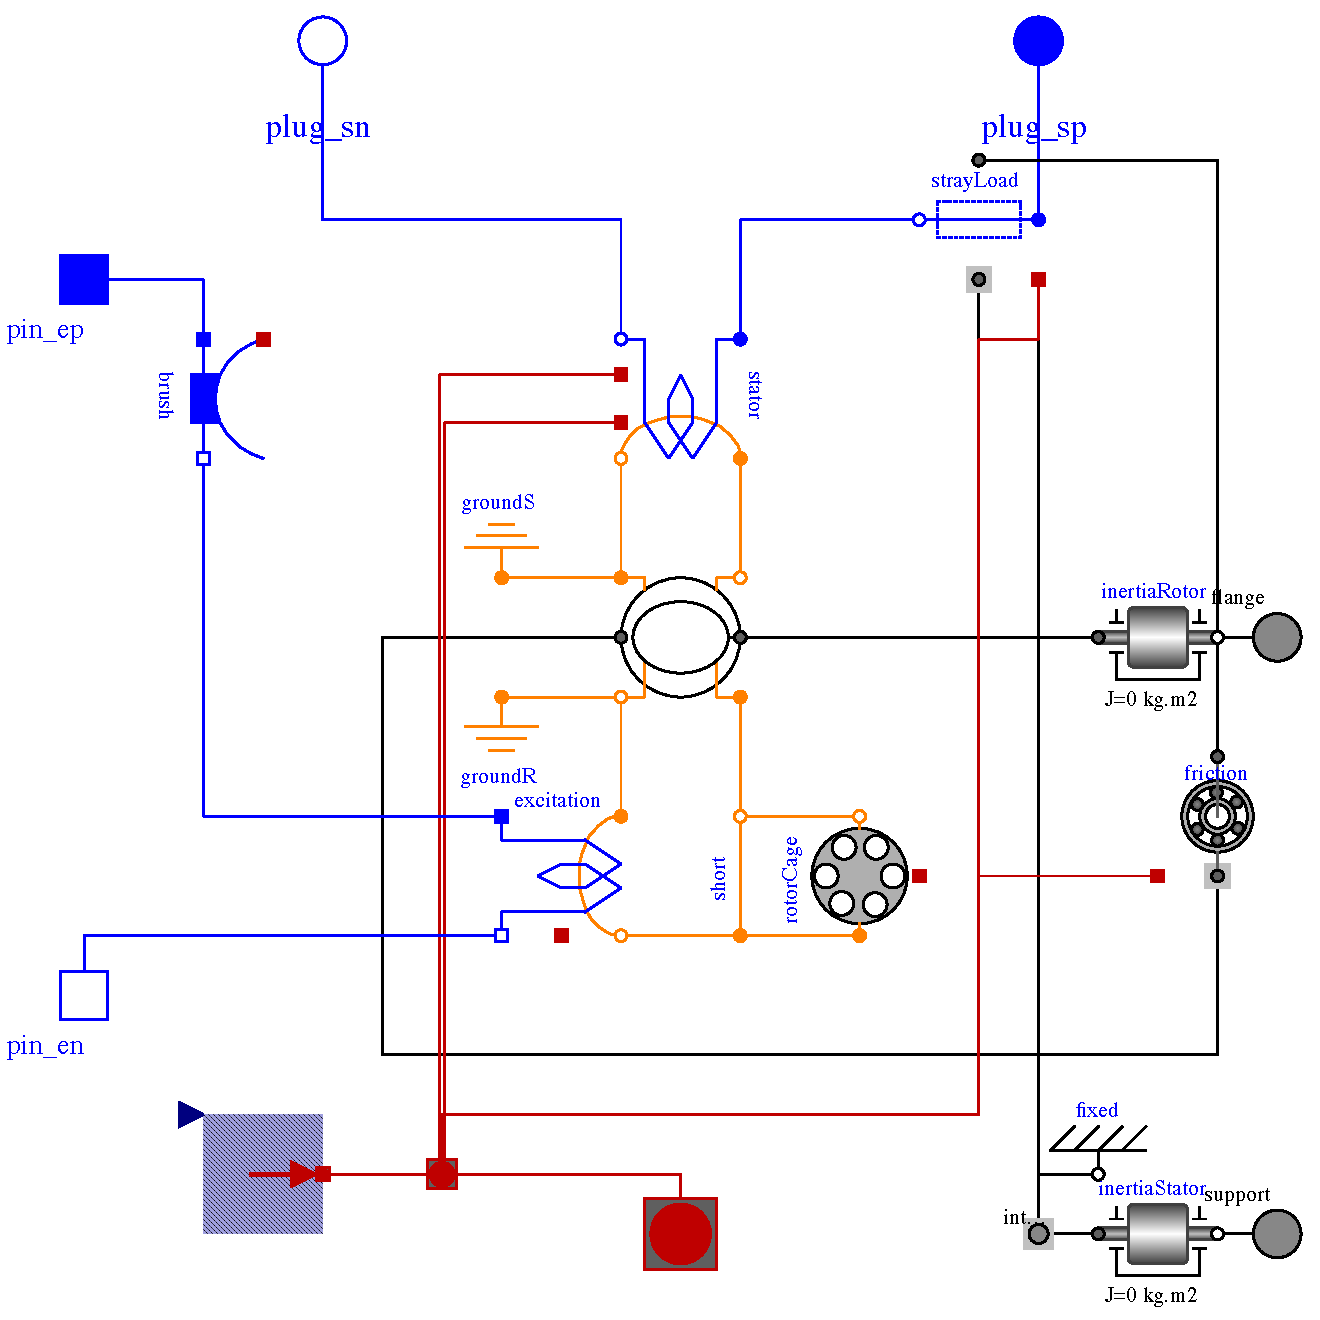
\includegraphics[]{Bilder/SM_ElectricalExcited.pdf}
    \caption{Vollständiges Modell des elektrisch erregten Synchrongenerators mit (optionalem) Dämpferkäfig (\modclass{Fun­da­men­tal­Wave.­Ba­sic­Ma­chines.­Syn­chro­nous­In­duc­tion­Ma­chines.­SM\_­E­lec­tri­cal­Ex­ci­ted}) der MSL v3.2.3}
    \label{fig:Synchrongenerator}
\end{figure}

Wie das mehrphasige Windungsmodell des Stators
berücksichtigt auch das einphasige Modell (\modclass{FundamentalWave.­Ba­sic­Ma­chines.­Com­po­nents.­Sin­gle­Phase­Win­ding}) neben der elektromagnetischen
Kopplung ohmsche Verluste und den magnetischen Streufluss.
% \begin{figure}
%     \centering
%     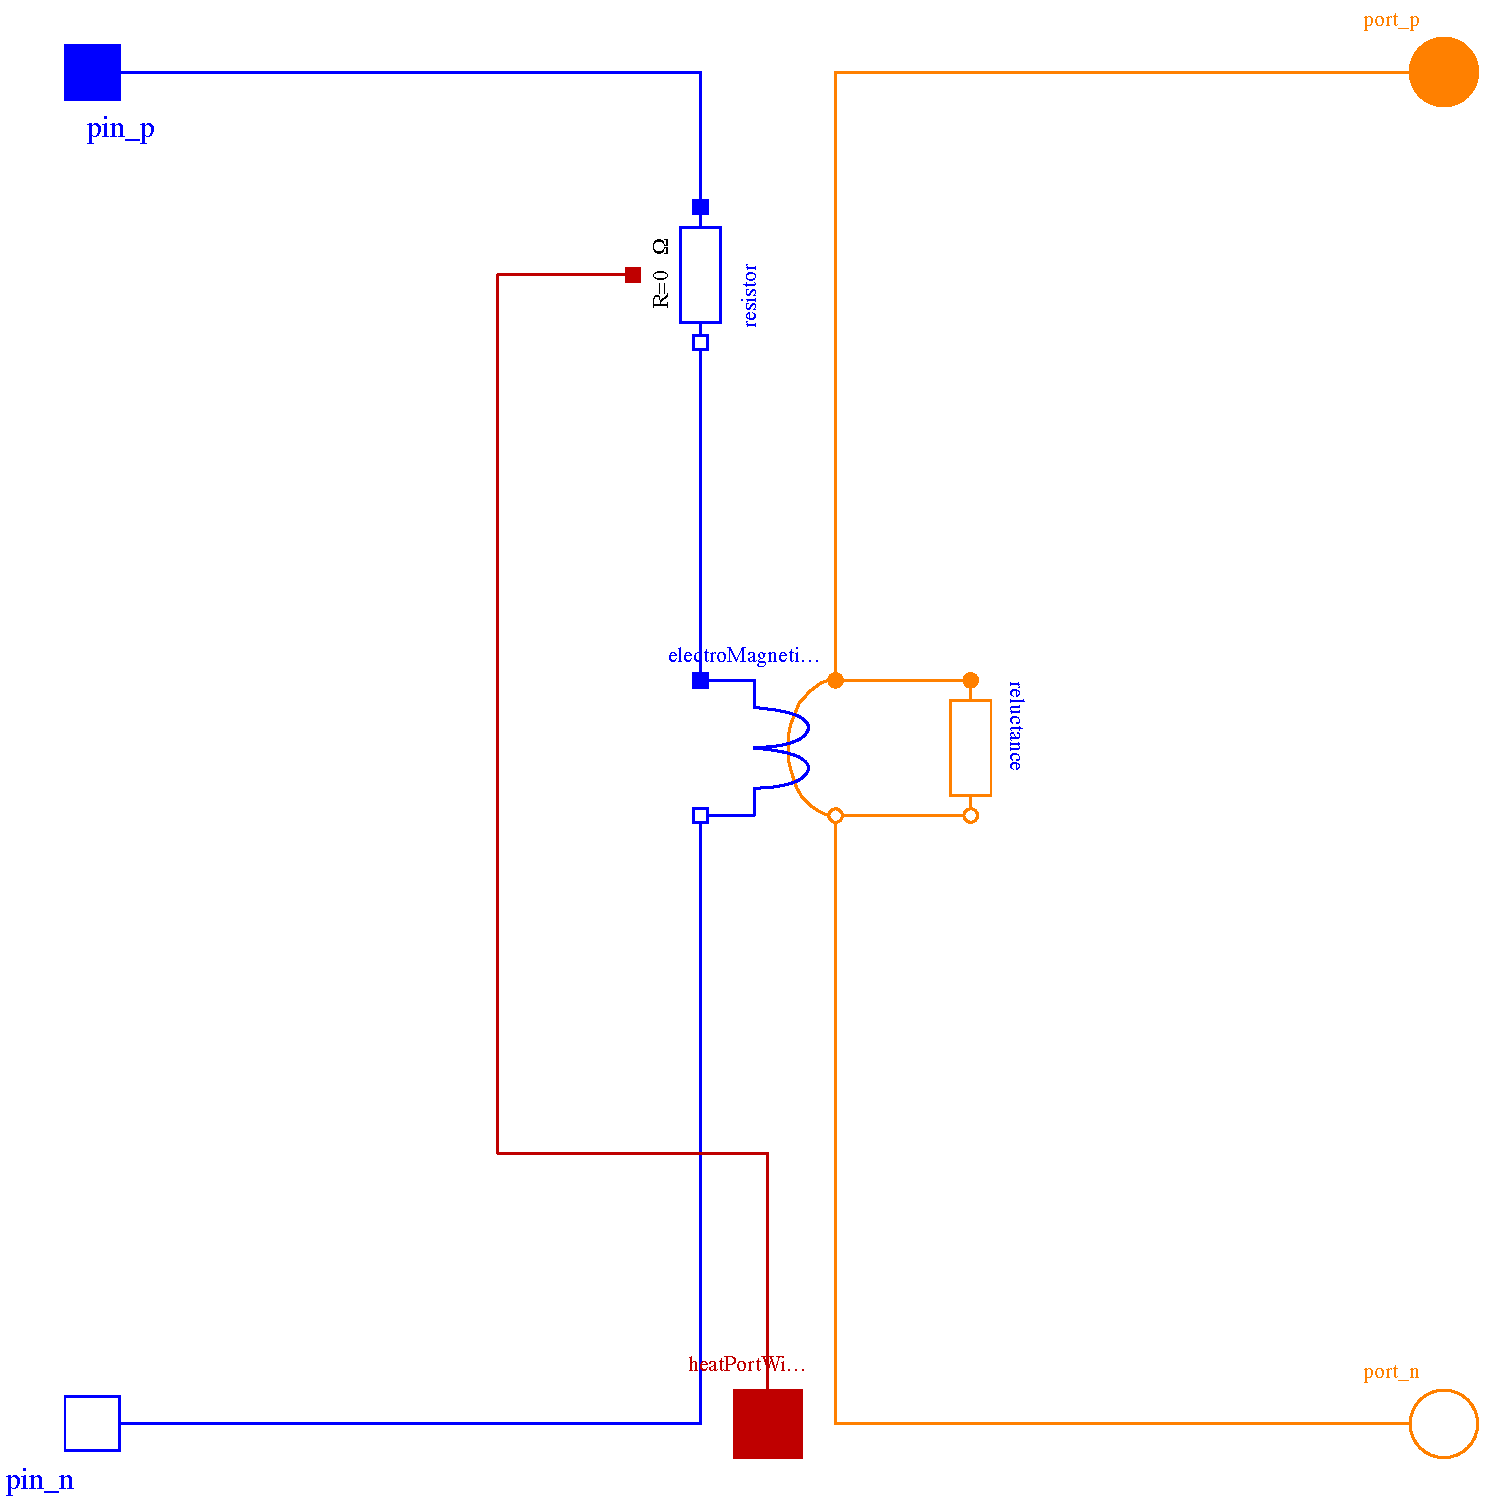
\includegraphics{Bilder/SinglePhaseWinding.pdf}
%     \caption{Einphasiges Windungsmodell (\modclass{FundamentalWave.­Ba­sic­Ma­chines.­Com­po­nents.­Sin­gle­Phase­Win­ding}) der MSL v3.2.3}
%     \label{fig:EinphasigesWicklungsmodell}
% \end{figure}

Da der Synchrongenerator über die Erregermaschine erregt wird, findet
keine Stromübertragung über Kohlebürsten statt und das Modell der
Kohlebürsten soll hier nicht beschrieben werden. Weiterhin beträgt der
Spannungsabfall über den Kohlebürsten in der Voreinstellung Null Volt.
Daher brauchen für die Kohlebürsten keine Parameter angegeben zu werden,
um einen Einfluss auszuschließen.

Das Modell des Dämpferkäfigs (\modclass{XXX}) weist die gleiche Struktur auf
wie der oben beschriebene Kurzschlussläufer. Im Unterschied zu diesem
berücksichtigt das Dämpferkäfigmodell hingegen die Achsigkeit (d- und
q-Achsen des körperfesten Koordinatensystems) der Widerstände und
Induktivitäten aufgrund der Pollücken des Dämpferkäfigs
(\cite[S. 194]{kralModelicaObjektorientierteModellbildung2019}).
Dementsprechend ist das Modell zweiphasig ausgeführt.
% \begin{figure}
%     \centering
%     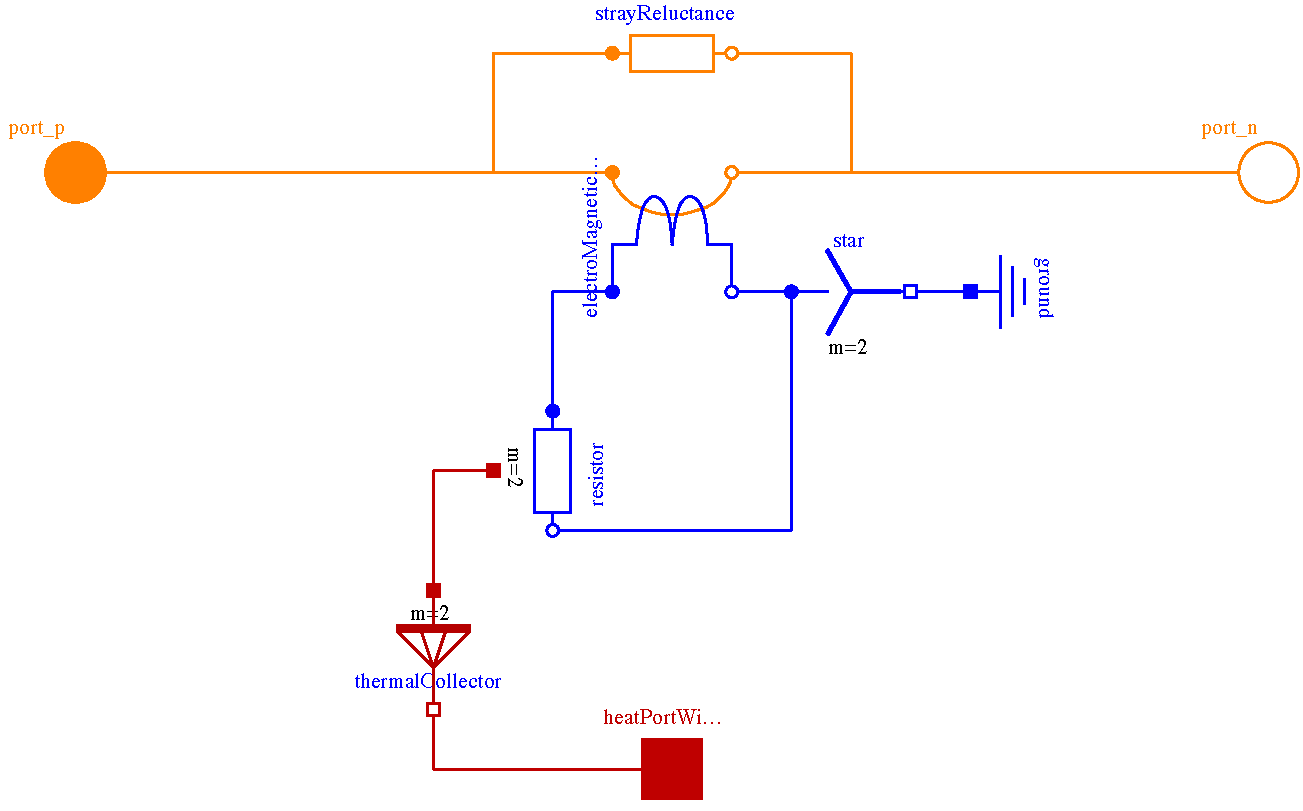
\includegraphics{Bilder/SaliencyCageWinding.pdf}
%     \caption{Caption}
%     \label{fig:SaliencyCageWinding}
% \end{figure}

\subsubsection{Parametrierung}\label{parametrierung-SG}

Alle Parameter des Synchrongenerators werden in dem Parameterrecord
\modclass{Ma­chines.­U­ti­li­ties.­Pa­ra­me­ter­Re­cords.­SM\_­E­lec­tri­cal­Ex­ci­ted­Da­ta}
der MSL v3.2.3 erfasst. Die mechanischen und thermischen Parameter des
Synchrongenerators sind dieselben wie die der Asynchronmaschine: Die
Temperaturen betragen \(\unit[20]{^\circ C}\) Umgebungstemperatur bei
Vernachlässigung der Temperaturabhängigkeit der Widerstände und das
Trägheitsmoment wird ebenfalls in dem kombinierten Trägheitsmoment des
Lüfters erfasst.

Die zur Parametrierung des Synchrongenerators verwendeten elektrischen
Größen sind die im Erstzschaltbild \cref{XXX} angegebenen Widerstände und
Induktivitäten. Aus der Auslegung der Maschine hingegen sind die in
Tabelle \cref{XXX} aufgelisteten Größen bekannt. Die zur Umrechnung benötigten Zusammenhänge sollen im Folgenden angegeben werden. Zwar sind die hier angegebenen Zusammenhänge zum größten Teil auch in dem Parameterrecord \modclass{Machines.Utilities.SynchronousMachineData} implementiert, jedoch erfordert der Parameterrecord die Kenntnis der Ankerzeitkonstante \(T_{\mathrm{a}}\) zur Berechnung des Statorwiderstands \(R_{\mathrm{s}}\). Da jedoch \(R_{\mathrm{s}}\) (im Gegensatz zu \(T_{\mathrm{a}}\)) aus der Auslegung bekannt ist, erfolgt hier diese angepasste Umformung der Kenngrößen.

Nach \cite[S. 264]{kralModelicaObjektorientierteModellbildung2019} können die bezogenen Hauptfeldreaktanzen \(x_{\mathrm{md}}\) und \(x_{\mathrm{mq}}\) mit
\begin{align}
    x_{\mathrm{md}} &= x_{\mathrm{d}} - x_{\mathrm{s}} \\
    x_{\mathrm{mq}} &= x_{\mathrm{q}} - x_{\mathrm{s}}
\end{align}
aus den bezogenen Reaktanzen \(x_{\mathrm{d}}\) und \(x_{\mathrm{q}}\) sowie der Streureaktanz \(x_{\mathrm{s}}\) bestimmt werden. An dieser Stelle verwendet \cite[]{kralModelicaObjektorientierteModellbildung2019} anstelle von \(x_{\mathrm{s}}\) die Nullreaktanz \(x_{\mathrm{0}}\), die in etwa mit der Streureaktanz übereinstimmt. Da hier aber die Streureaktanz aus der Auslegung bekannt ist, soll \(x_{\mathrm{s}}\) direkt verwendet werden. 

Weiterhin wird dort die Reaktanz der Erregerwicklung gemäß
\begin{equation}
    x_{\mathrm{e}} = \frac{x_{\mathrm{md}}^2}{x_{\mathrm{d}}-x_{\mathrm{d}}'}
\end{equation}
angegeben. Ebenso seien die Zusammenhänge für die bezogenen Rotorreaktanzen \(x_{\mathrm{rd}}\) und \(x_{\mathrm{rq}}\)
\begin{align}
    x_{\mathrm{rd}} &= \frac{x_{\mathrm{md}}^2}{x_{\mathrm{d}}' - x_{\mathrm{d}}''}\cdot \left( 1-\frac{x_{\mathrm{md}}}{x_{\mathrm{d}}}\right)^2 + \frac{x_{\mathrm{md}}^2}{x_{\mathrm{e}}}\\
    \intertext{und}
    x_{\mathrm{rq}} &= \frac{x_{\mathrm{mq}}^2}{x_{\mathrm{q}} - x_{\mathrm{q}}''}.
\end{align}
Für die bezogenen Rotorwiderstände\footnote{An dieser Stelle liegt in der vorliegenden Ausgabe von \cite[]{kralModelicaObjektorientierteModellbildung2019} ein Druckfehler vor (vgl. mit dem Modelica-Code Listing \cite[S. 266]{kralModelicaObjektorientierteModellbildung2019})} wird ebenda
\begin{align}
    r_{\mathrm{rd}} &= \frac{x_{\mathrm{rd}} - \frac{x_{\mathrm{md}}^2}{x_{\mathrm{e}}}}{\omega_{\mathrm{sN}}\cdot T_{\mathrm{d0}}''}, \\
    r_{\mathrm{rq}} &= \frac{x_{\mathrm{rq}}}{T_{\mathrm{q0}}''}
\end{align}
angegeben und für den bezogenen Widerstand der Erregerwicklung
\begin{equation}
    r_{\mathrm{e}} = \frac{x_{\mathrm{e}}}{\omega_{\mathrm{sN}}\cdot T_{\mathrm{d0}}''}.
\end{equation}
Die beiden Subtransienten Leerlaufzeitkonstanten \(T_{\mathrm{d0}}''\)
und \(T_{\mathrm{q0}}''\) sind nach
\cite[S. 222ff.]{bonfertBetriebsverhaltenSynchronmaschine1962} über den Zusammenhang
\begin{align}
T_{\mathrm{d0}}'' &= \frac{x_{\mathrm{d}}'}{x_{\mathrm{d}}''}T_{\mathrm{d}}'' \\
T_{\mathrm{q0}}'' &= \frac{x_{\mathrm{q}}}{x_{\mathrm{q}}''}T_{\mathrm{q}}
\end{align}
aus den Kurzschlusszeitkonstanten \(T_{\mathrm{d}}''\) und
\(T_{\mathrm{q}}''\) berechenbar.

Damit ergeben sich die Induktivitäten und Widerstände des
Synchrongenerators mit der Nennkreisfrequenz
\(\omega_{\mathrm{sN}}=2\pi\cdot f_{\mathrm{sN}}\) und der
Bezugsreaktanz \(X_{\mathrm{N}}\) nach Gleichungen XXX (vgl.
\cite[S.265f.]{kralModelicaObjektorientierteModellbildung2019}).
\begin{align}
L_{\mathrm{md}} &= x_{\mathrm{md}}\cdot \frac{X_{\mathrm{N}}}{\omega_{\mathrm{sN}}} \\
L_{\mathrm{mq}} &= x_{\mathrm{mq}}\cdot \frac{X_{\mathrm{N}}}{\omega_{\mathrm{sN}}} \\
L_{\mathrm{r \sigma d}} &= (x_{\mathrm{rq}}-x_{\mathrm{mq}})\cdot \frac{X_{\mathrm{N}}}{\omega_{\mathrm{sN}}} \\
L_{\mathrm{r \sigma q}} &= (x_{\mathrm{rd}}-x_{\mathrm{md}})\cdot \frac{X_{\mathrm{N}}}{\omega_{\mathrm{sN}}} \\
L_{\mathrm{s \sigma}} &= x_{\mathrm{s}}\cdot \frac{X_{\mathrm{N}}}{\omega_{\mathrm{sN}}} \\
R_{\mathrm{rd}} &= r_{\mathrm{rd}}\cdot X_{\mathrm{N}} \\
R_{\mathrm{rq}} &= r_{\mathrm{rq}}\cdot X_{\mathrm{N}} \\
R_{\mathrm{e}} &= \frac{3}{2}\cdot \left(\frac{\sqrt{2}V_{\mathrm{sN}}}{\omega_{\mathrm{sN}}L_{\mathrm{md}}\cdot I_{\mathrm{Err. Leerl.}}}\right)^2\cdot r_{\mathrm{e}}\cdot X_{\mathrm{N}}
\end{align}
Damit ist der Synchrongenerator vollständig parametriert. Die \cref{tab:AuslegungSG,tab:ZwischenwerteSG,tab:ParameterRecordSG,tab:ParameterSG} listen eine Übersicht über alle Parameter und Berechnungsgrößen auf.

\subsection{Erregermaschine}\label{sec:erregermaschine}

Die Erregermaschine und der auf dem Polrad der Maschine mitrotierende Gleichrichter dienen gemäß \cref{fig:Wirkungsgraph} der berührungslosen Erregung des Synchrongenerators über den Luftspalt. Wie bei dem Hauptgenerator handelt es sich auch bei der Erregermaschine um eine Synchronmaschine. Neben der geringeren Größe (ermöglicht durch die geringere Übertragungsleistung) unterscheiden sich die beiden Generatoren darin, dass die Erregermaschine eine Innenpol- und der Hauptgenerator eine Außenpolmaschine ist. In der Modellierung der Maschinen braucht dieser Umstand jedoch nicht berücksichtigt zu werden.

\subsubsection{Modell}\label{modell-erregermaschine}

\cref{fig:Erregermaschine} zeigt das vollständige Modell der in der \modclass{Frequenzumformer}-Bibliothek implementierten Erregermaschine. Als Generatormodell wird dasselbe Synchrongeneratormodell der MSL wie für den Hauptgenerator verwendet. Das \modclass{delta}-Modell zwischen den beiden dreiphasigen Ausgängen des Generators bewirkt eine Verkettung der Ströme und Spannungen wie in einer Dreieckschaltung der Statorstränge.

Die Gleichrichtung der erzeugten dreiphasigen Spannung geschieht mit einem 6-Puls-Brückengleichrichter (siehe \cref{fig:Gleichrichter}). Am negativen Ausgang des Brückengleichrichters wird ein (\unit[0]{V}) Referenzpotential verschaltet, ohne das die Gleichungen für den elektrischen Kreis zwischen Erregermaschine und Synchrongenerator nicht eindeutig lösbar wären.

Die Dioden des Gleichrichter verwenden ein ideales Diodenmodell mit zwei linearen Arbeitsbereichen \emph{Sperrbetrieb} und \emph{Durchlassbetrieb}. Die Steigung der Diodenkennlinien in den beiden Arbeitsbereichen wird über den Leitwert \(G_{\mathrm{off}}\) im Sperrbetrieb und den Widerstand \(R_{\mathrm{on}}\) im Durchlassbetrieb eingestellt. Der Wechsel vom Sperrbetrieb in den Durchlassbetrieb findet bei Überschreiten der Flussspannung \(U_{\mathrm{F}}\) statt. Ebenso wird zurück in den Sperrbetrieb geschaltet, sobald die Flussspannung unterschritten wird.

\begin{figure}
    \centering
    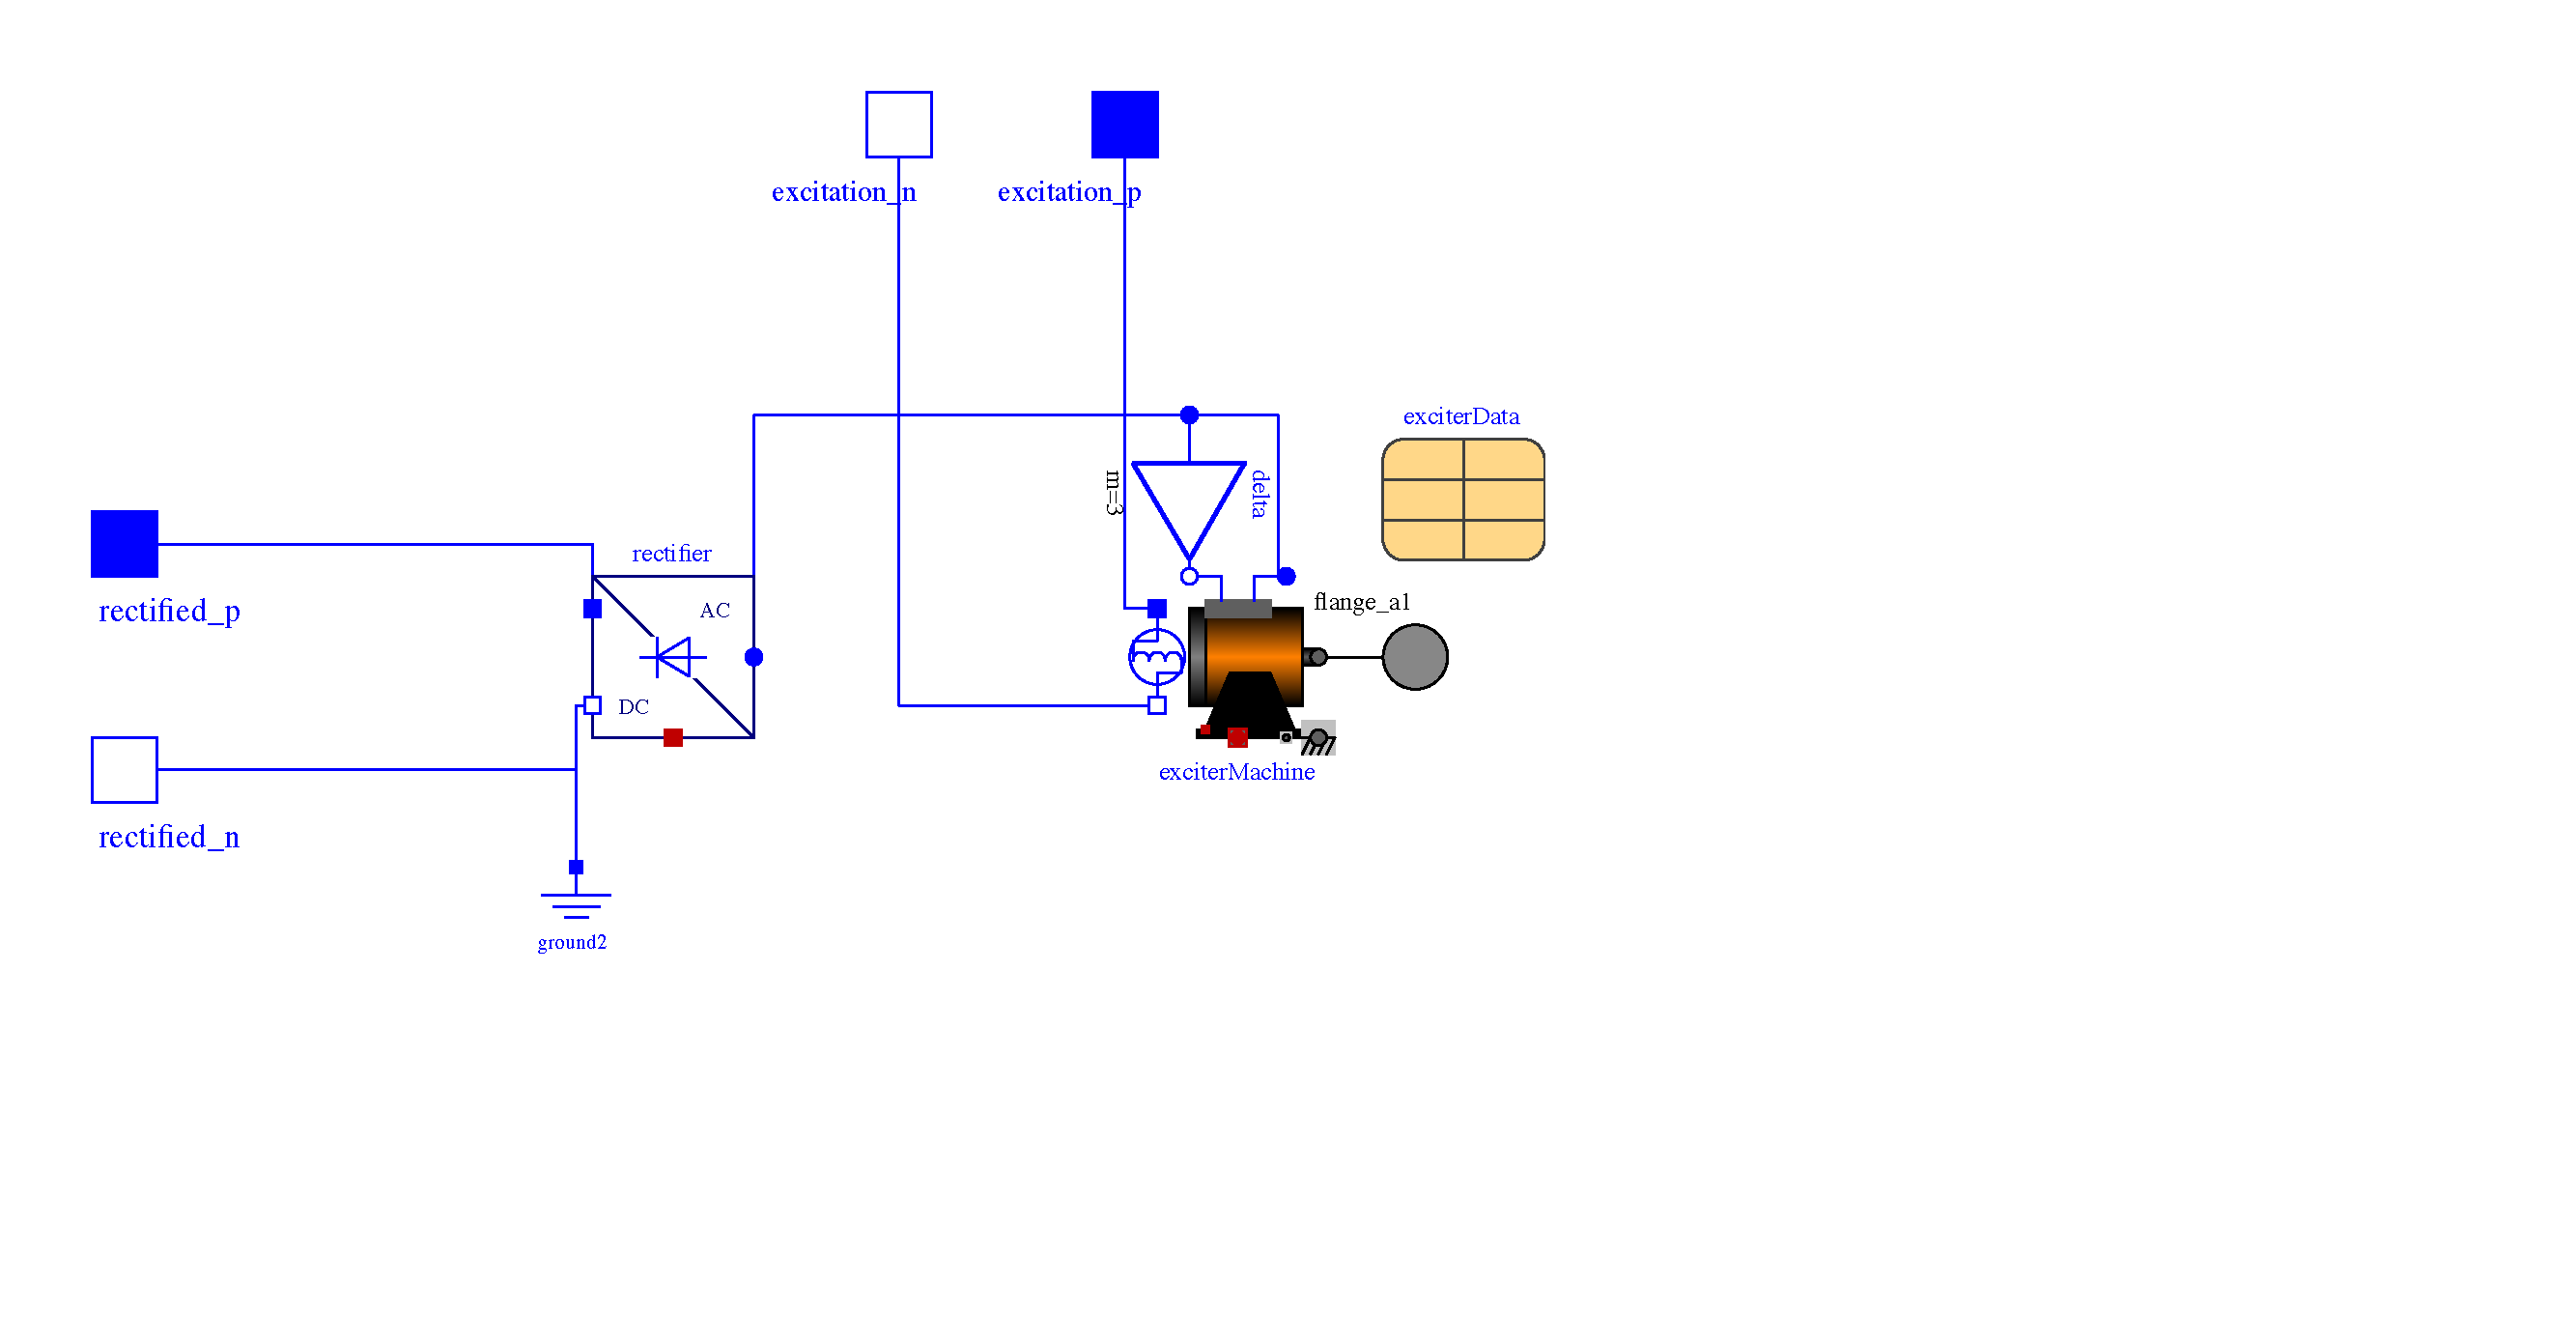
\includegraphics{Bilder/SM_Erreger.pdf}
    \caption{Vollständiges Modell der Erregermaschine}
    \label{fig:Erregermaschine}
\end{figure}

% \begin{figure}
%     \centering
%     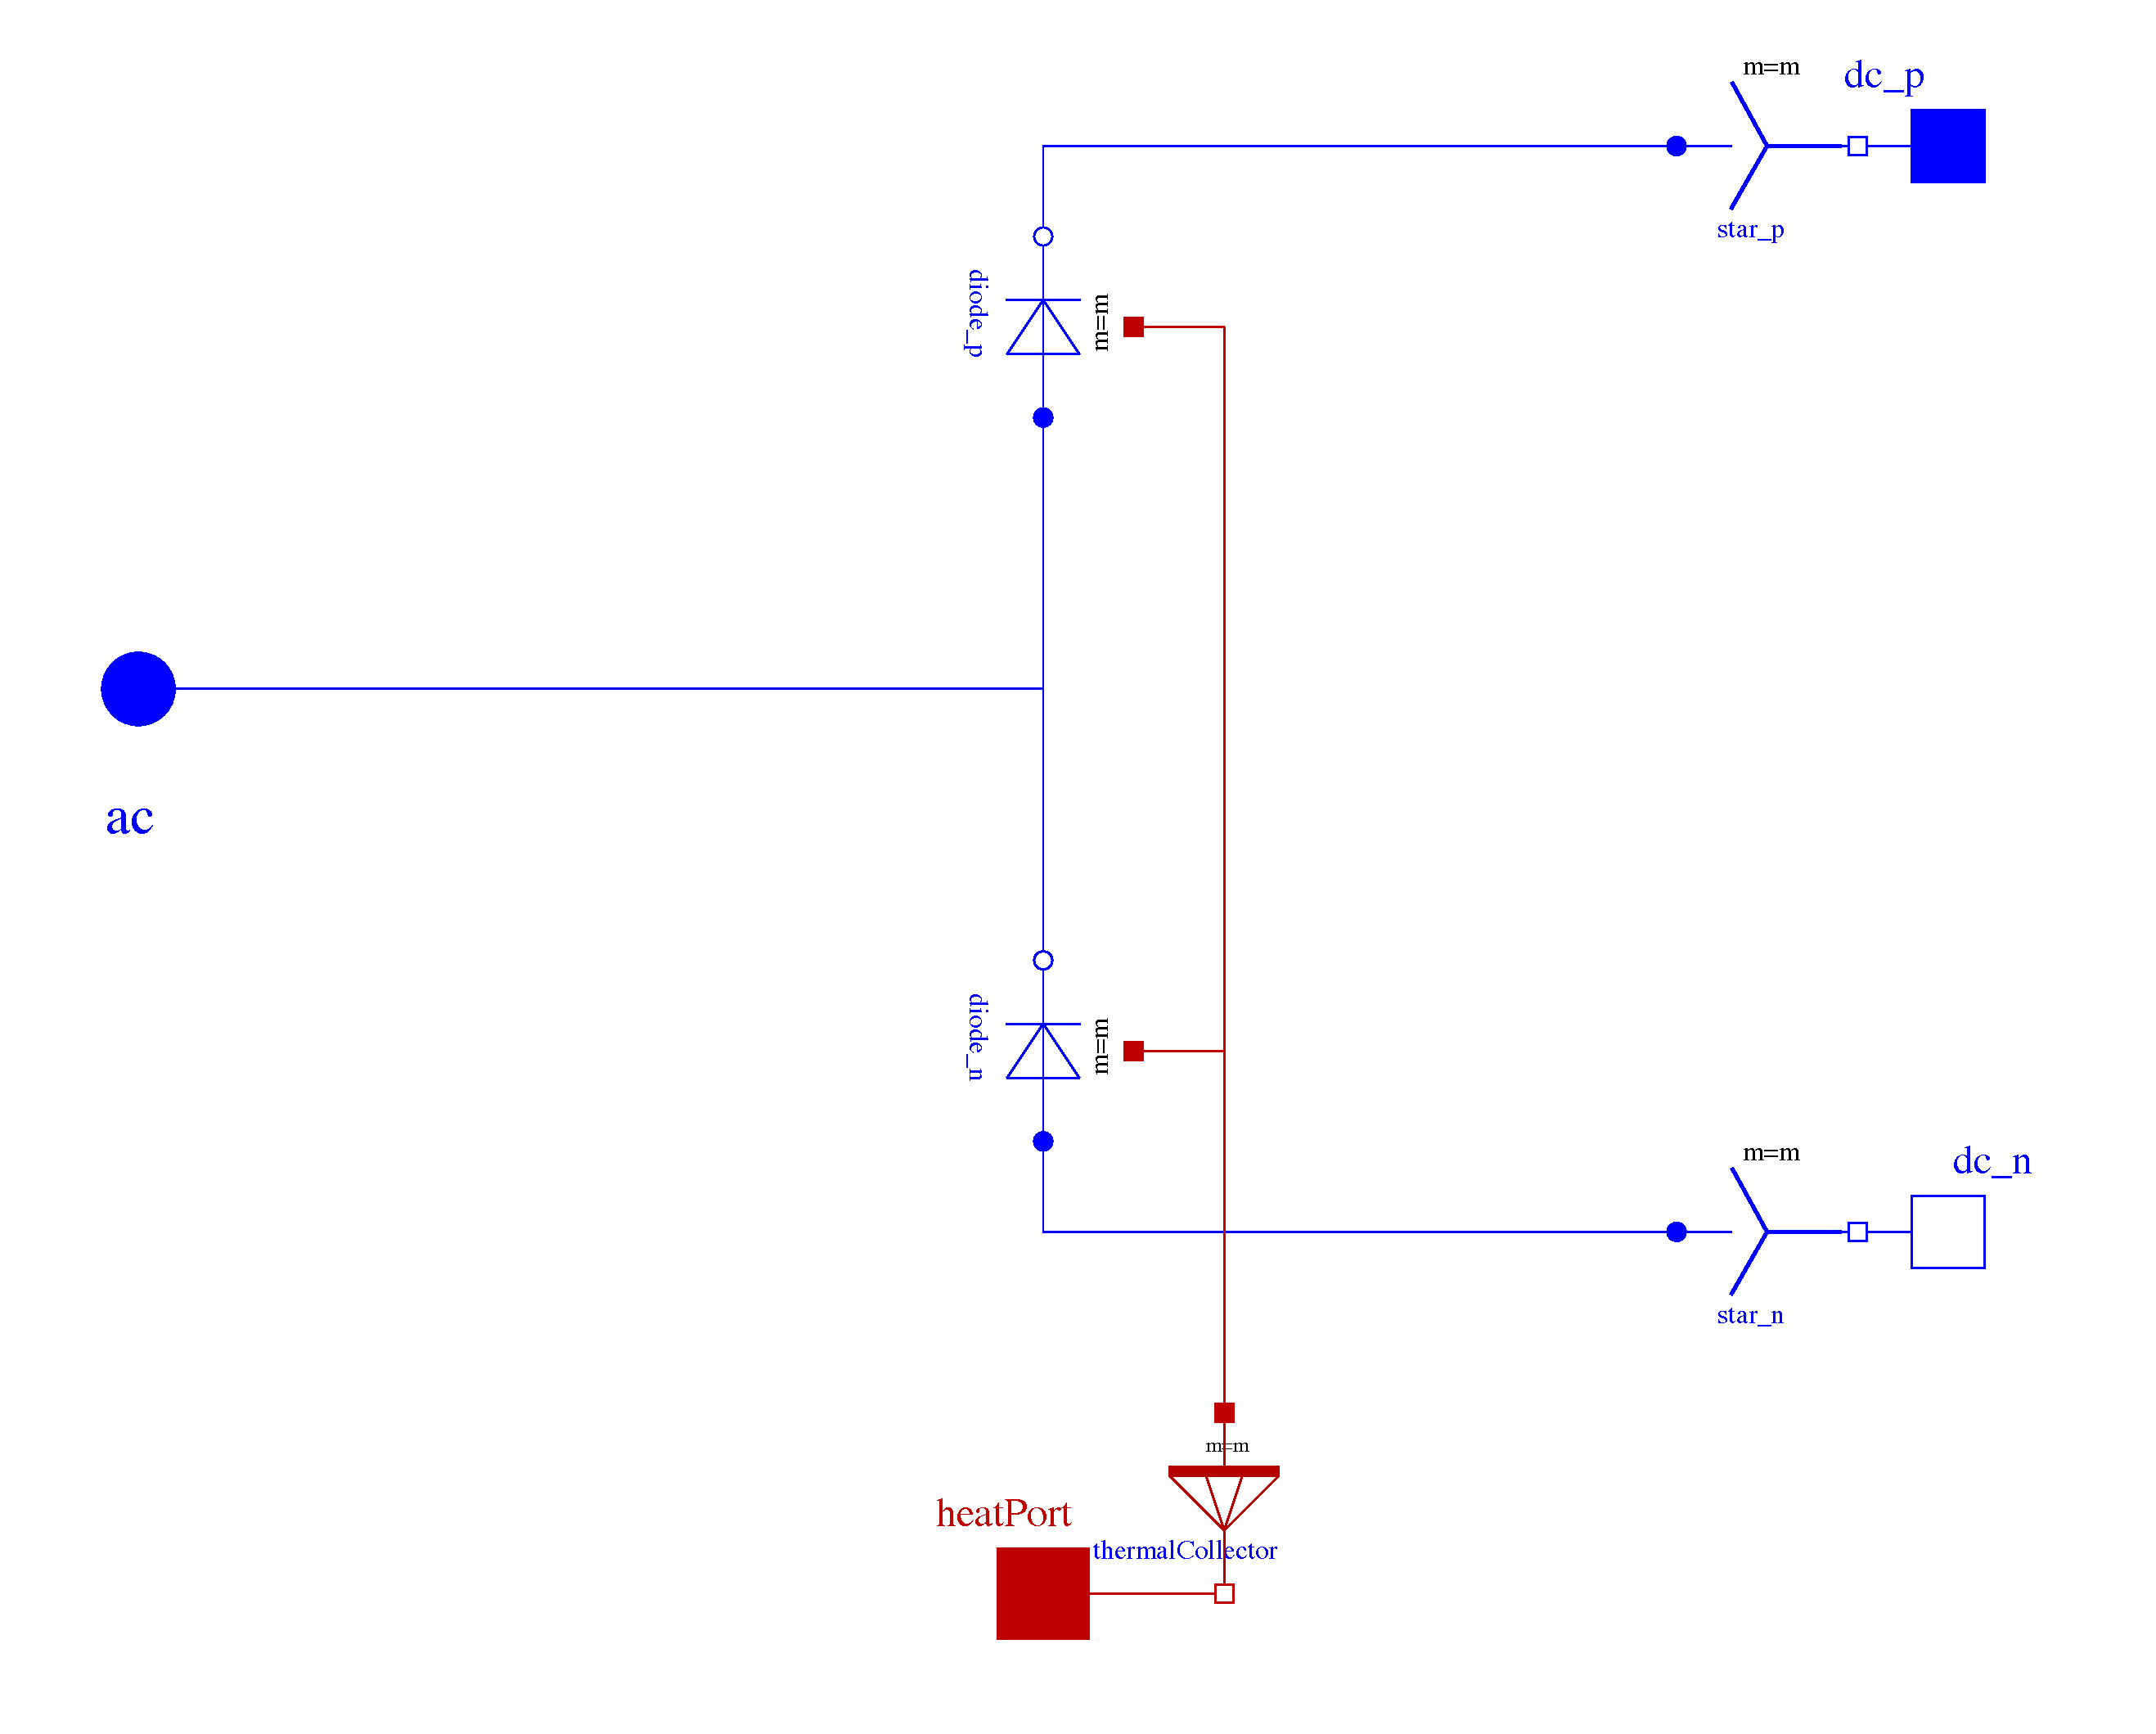
\includegraphics{Bilder/DiodeBridge2mPulse.pdf}
%     \caption{Vollständiges Modell des Dioden-Gleichrichters}
%     \label{fig:Gleichrichter}
% \end{figure}

\hypertarget{parametrierung-2}{%
\subsubsection{Parametrierung}\label{parametrierung-2}}

Die Parametrierung des Synchrongenerators der Erregermaschine erfolgt
analog zur Parametrierung des Hauptgenerators oben. Die verwendeten
Größen sind in  \cref{tab:AuslegungErregermaschine,tab:ParameterErregermaschine,tab:ParameterRecordErregermaschine,tab:ZwischenwerteErregermaschine} dargestellt.

Für den Brückengleichrichter sind aus der Auslegung keine Werte bekannt. Daher wird für die Flussspannung \(U_{\mathrm{F}}=\unit[0,7]{V}\) angenommen. Der Leitwert \(G_{\mathrm{off}}\) und der Widerstand \(R_{\mathrm{on}}\) einer idealen Diode betragen Null. Um jedoch numerische Probleme (Teilen durch Null bzw. Ansteigen der resultierenden Größen gegen Unendlich) zu vermeiden, werden \(G_{\mathrm{off}}=\unit[0,001]{S}\) bzw. \(R_{\mathrm{on}}=\unit[0,001]{\Omega}\) festgelegt, die nahe Null, aber noch groß genug sind um die genannten Probleme zu vermeiden.


\hypertarget{spannungsregler}{%
\subsection{Spannungsregler}\label{spannungsregler}}
Der Spannungsregler wird in Modelica als Signalflussobjekt implementiert. Zur Unterstützung des objektorientierten Ansatzes werden die Teilglieder des Reglers (P-Glied, I-Glied und D-Glied) als eigenständige Objekte definiert, die in dem Spannungreglermodell verwendet werden.

Wie im Blockschaltbild des Reglers (\cref{fig:Blockschaltbild_Regler}) dargestellt ist allen Regelgliedern ein Begrenzer nachgeschaltet. Dies trägt zum Einen der Abbildung der Messgrößen auf das begrenzte Intervall der reglerinternen Größen Rechnung und bietet zum Anderen die Möglichkeit die Stellgrößen der Regelglieder unabhängig voneinander zu begrenzen. Um diese Begrenzung bei allen Gliedern mit einer einheitlichen Schnittstelle zu implementieren wird aus dem \textbf{S}ingle-\textbf{I}nput-\textbf{S}ingle-\textbf{O}utput-Interface der MSL (\modclass{Modelica.Blocks.Interfaces.SISO}) das Interface \modclass{Frequenzumformer.Regler.Interfaces.limitedController} abgeleitet, welches die Begrenzungsgrößen zugänglich macht. Weiterhin wird in dem Interface der boolsche Eingang \modclass{enable} definiert zum Einschalten des jeweiligen Regelgliedes.

\paragraph{Modell}\label{modell-Regler}
Das vollständige Modell des Spannungsreglers zeigt \cref{fig:Spannungsregler-Modell}. Es enthält die drei Teilglieder des PID-Reglers, die Stellgrößenbeschränkung und am Ausgang einen Schalter um den Wert Null auszugeben, wenn der Regler ausgeschaltet ist.
%TODO: Parametrierung des Reglers (Herleitung aus Z-Transformation) beschreiben
\begin{figure}
    \centering
    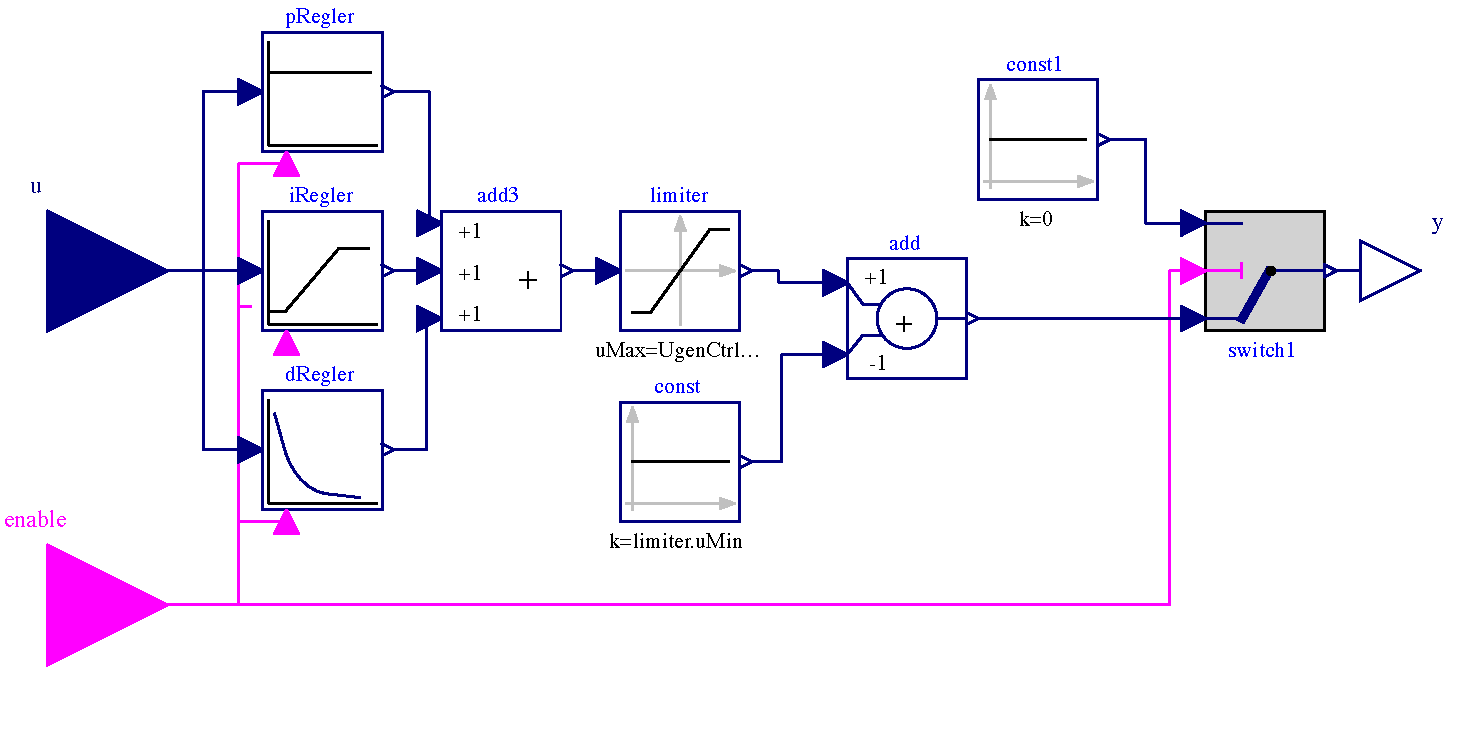
\includegraphics{Bilder/Spannungsregler.pdf}
    \caption{Vollständiges Modell des Spannungsreglers (\modclass{Fre­quenz­um­for­mer.­Reg­ler.­Span­nungs­reg­ler})}
    \label{fig:Spannungsregler-Modell}
\end{figure}

\begin{figure}
\centering
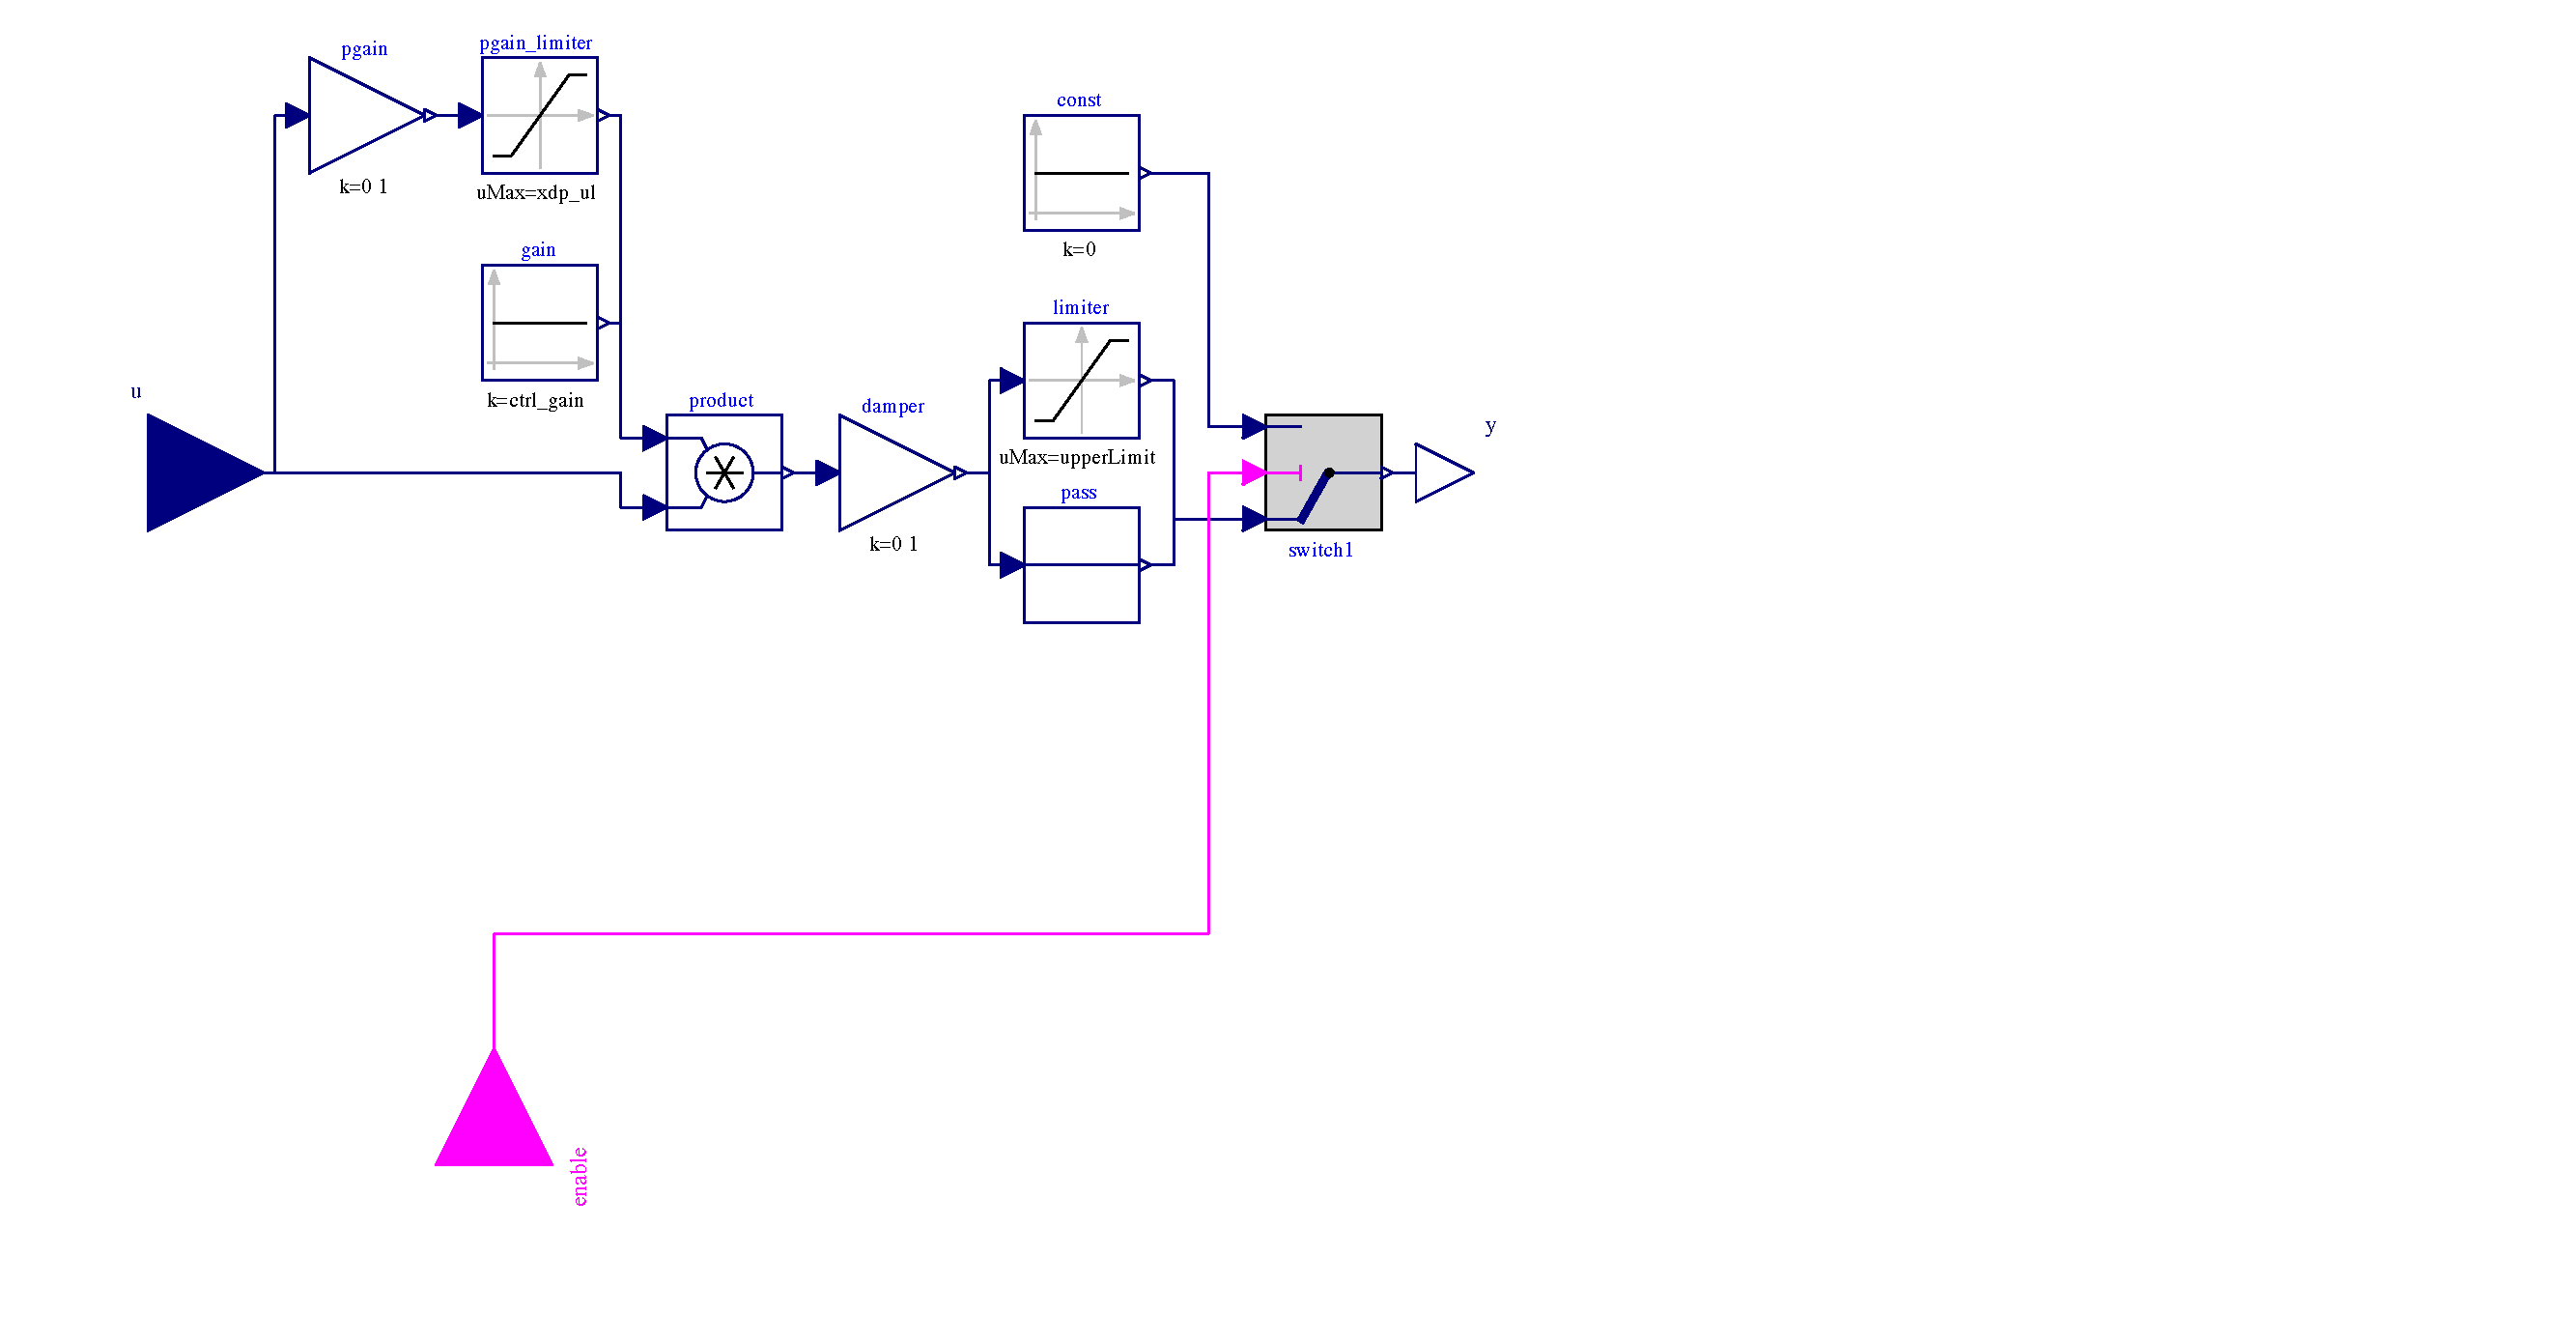
\includegraphics{Bilder/PRegler.pdf}
\caption{Modell des Proportional-Reglers (\modclass{Fre­quenz­um­for­mer.­Reg­ler.­Kon­ti­nu­ier­lich.­PRegler})}
\end{figure}

\begin{figure}
\centering
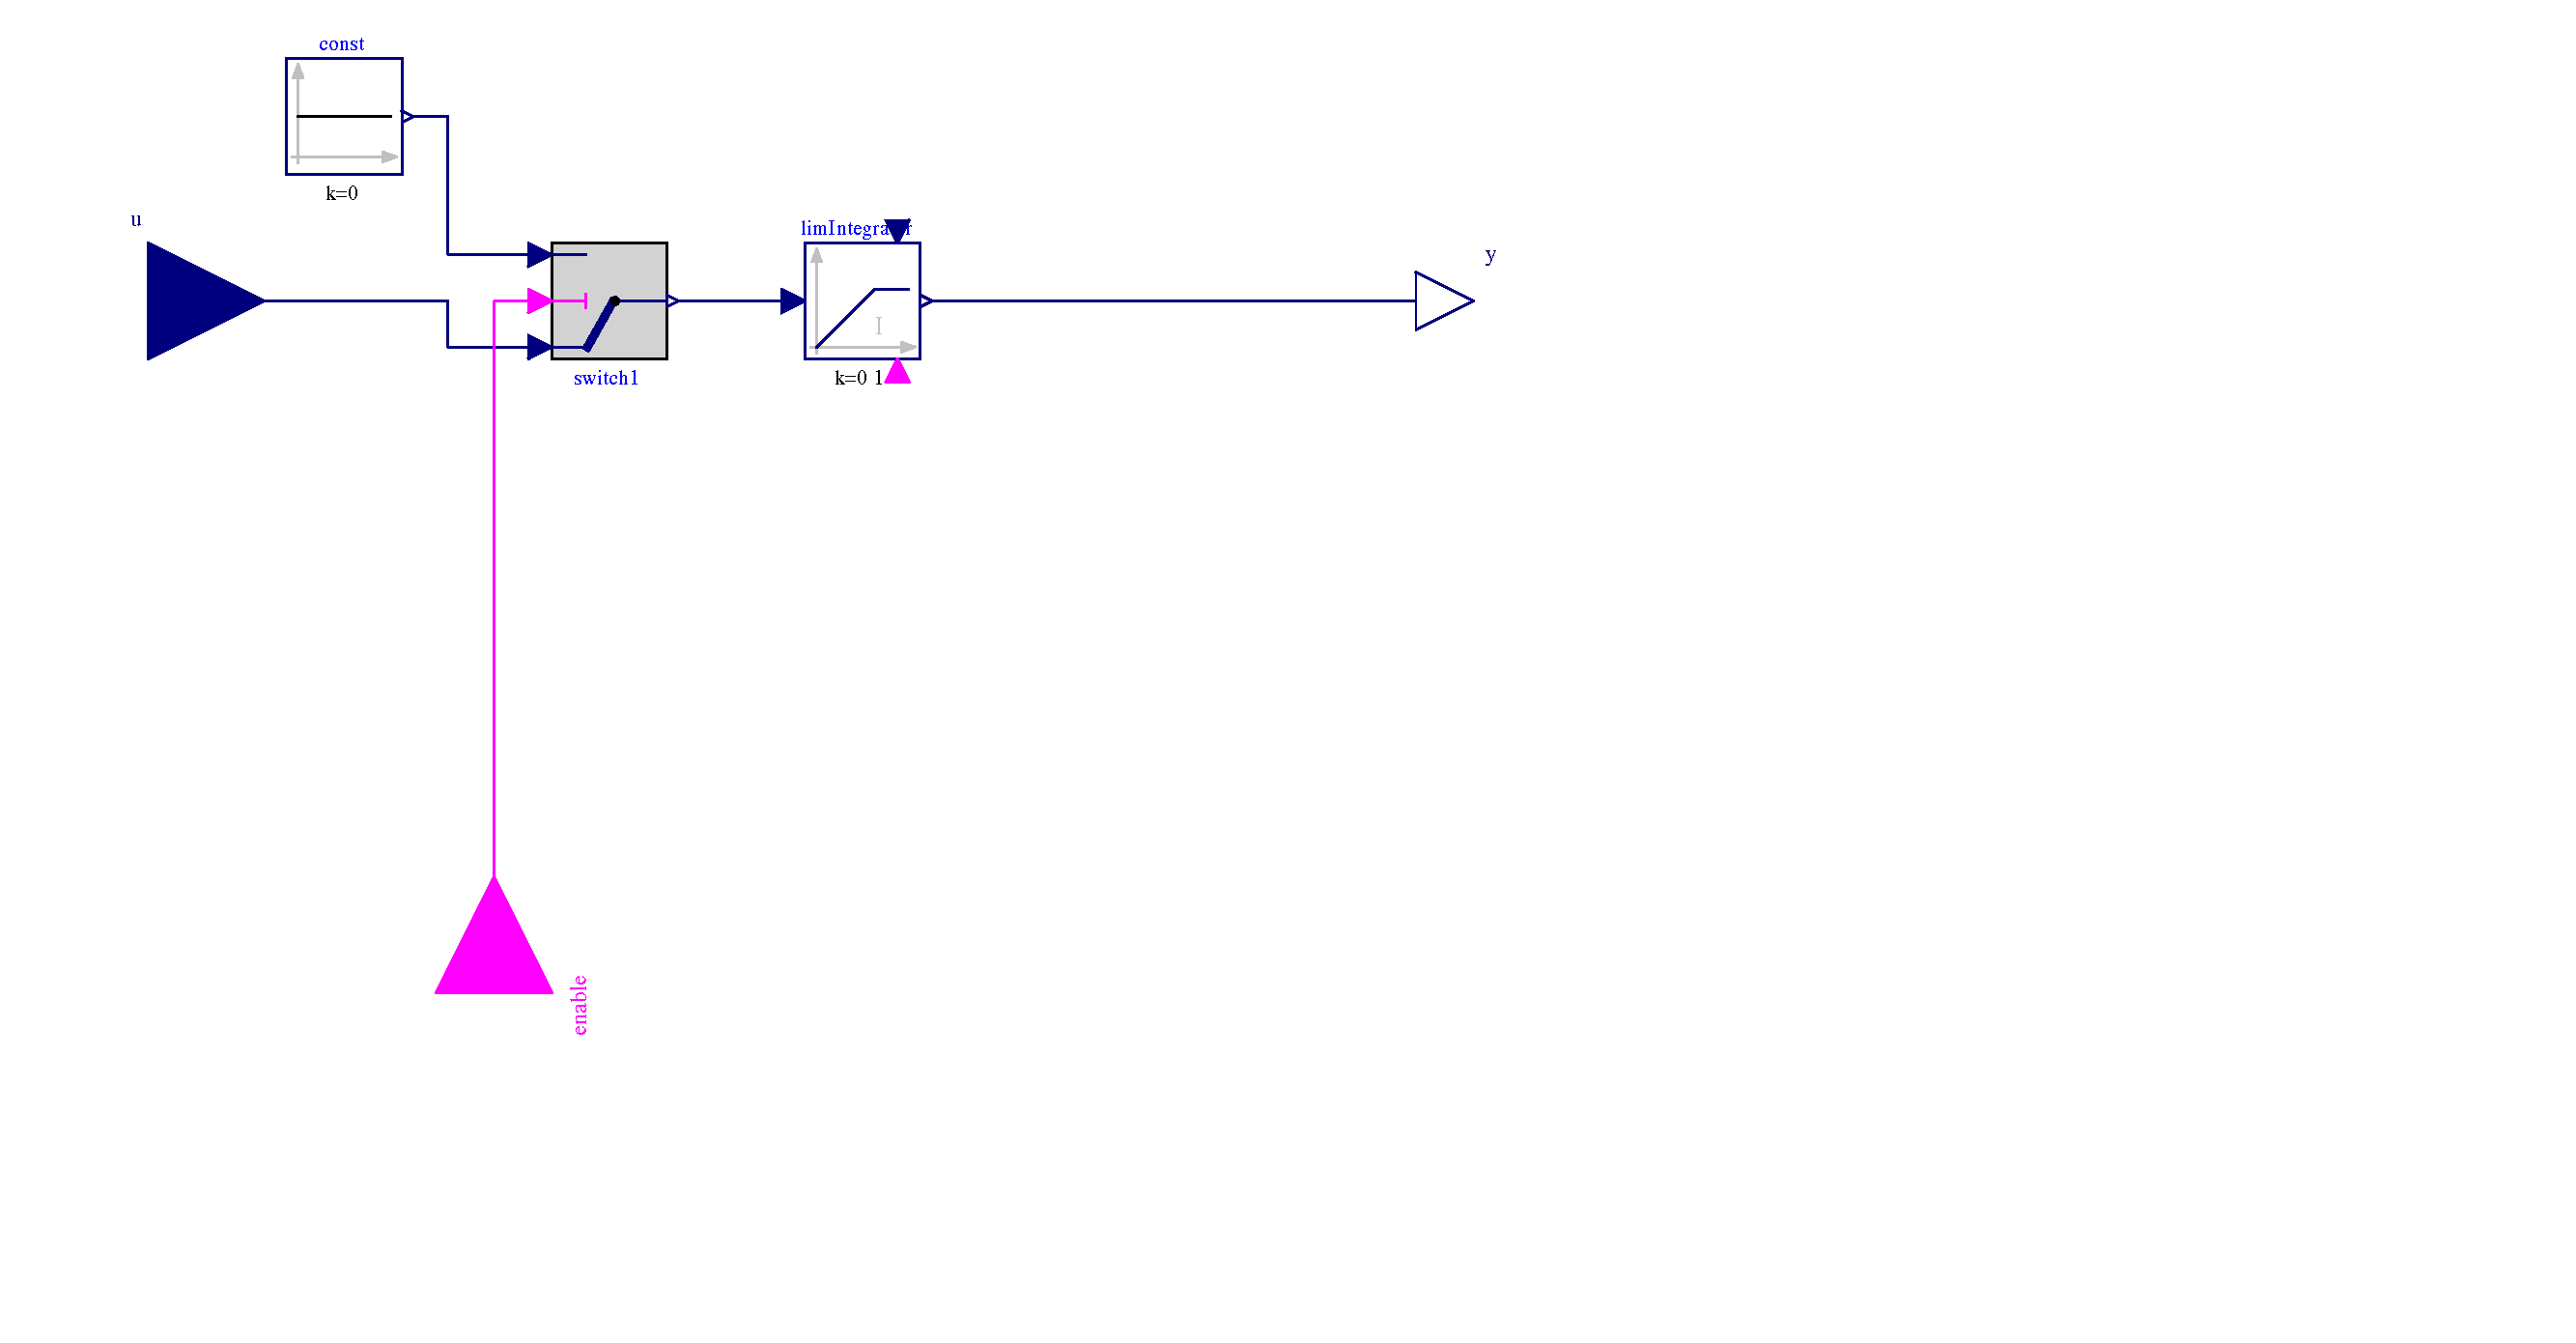
\includegraphics{Bilder/IRegler.pdf}
\caption{Modell des I-Reglers (\modclass{Fre­quenz­um­for­mer.­Reg­ler.­Kon­ti­nu­ier­lich.­IRegler})}
\end{figure}

\begin{figure}
    \centering
    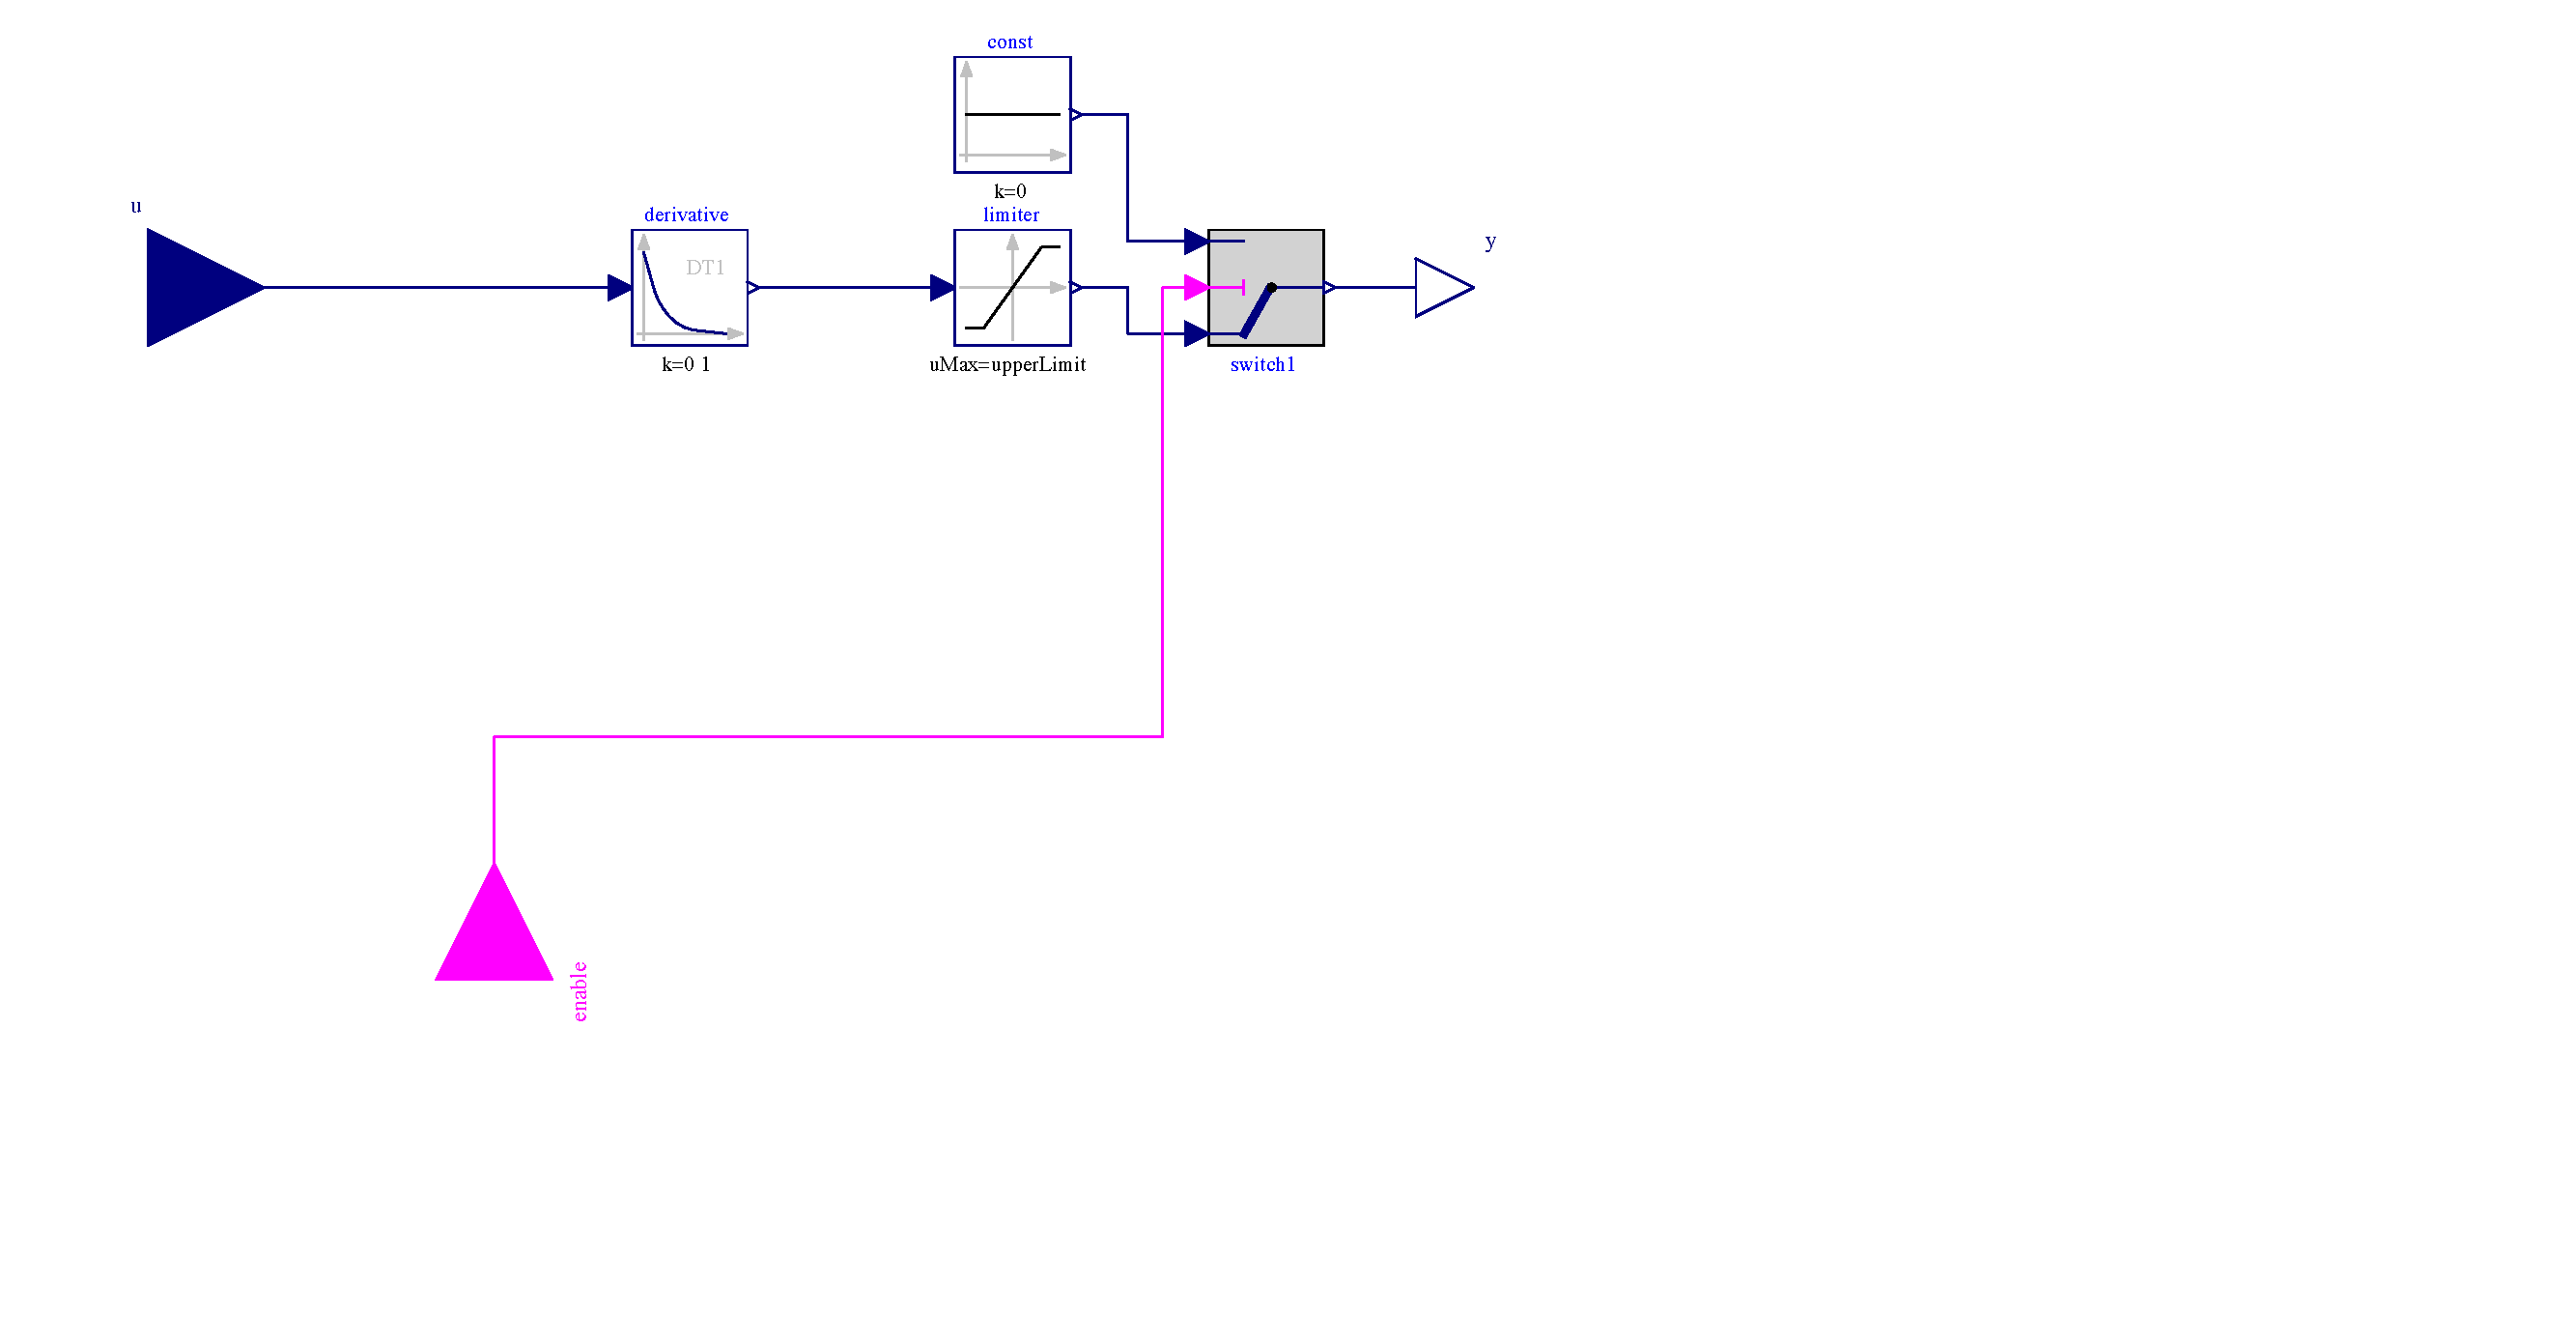
\includegraphics[]{Bilder/DRegler.pdf}
    \caption{Modell des D-Reglers (\modclass{Fre­quenz­um­for­mer.­Reg­ler.­Kon­ti­nu­ier­lich.­DRegler})}
    \label{fig:D-Regler}
\end{figure}

\subsection{Umwandlung der reglerinternen Stellgröße}
\label{sec:umwandlungenStellgrosse}
%TODO: Offset-Map beschreiben

\subsection{Weitere Modelle}\label{weitere-modelle}


\subsubsection{Leistungsmessung}\label{leistungsmessung}
%TODO: Leistungsmessung beschreiben

\subsubsection{Parametrierung der Last}\label{parametrierung-der-last}
%TODO: Parametrierung der Last beschreiben

\subsection{Gesamtmodell}\label{gesamtmodell}
\afterpage{%
%TODO: Entkommentieren
%\begin{landscape}
\begin{figure}
    \centering
    \oldincludegraphics[width=\linewidth]{Bilder/Umformer.pdf}
    \caption{Vollständiges Modell des Umformers}
\end{figure}
%\end{landscape}
}
%TODO: Gesamtmodell beschreiben
\hypertarget{initialisieren-des-modells}{%
\subsection{Initialisieren des
Modells}\label{initialisieren-des-modells}}

\chapter{Messungen am Frequenzumformer}
\label{chap:Versuch}
In diesem Kapitel sollen der Messaufbau und die Auswertung der Messergebnisse des Frequenzumformers beschrieben werden. Mit Hilfe der Messungen wird dann in \cref{chap:VerfikationValidierung} das Modelica-Modell mit der elektrischen Anlage abgeglichen. Schließlich werden die Ergebnisse des ParameterSweeps in \cref{chap:Auswertung} mit den Ergebnissen der Messreihen verglichen. 

Aufgenommen wurden Zeitverläufe der Spannungen und Ströme an den Ein- und Ausgängen des Umformers, sowie am Ausgang des Spannungsreglers und des mitrotierenden Gleichrichters. Verwendet wurde dazu eine Standardmesseinrichtungen mit Lastbank für Typ- und Serienprüfungen elektrischer Anlagen der Fa. Piller Power Systems. 

Im Folgenden wird zunächst dieser Messaufbau beschrieben. Anschließend folgt ein Überblick über die aufgenommenen Daten und deren Aufbereitung und Auswertung.

\section{Messaufbau}
\label{sec:Messaufbau}
Die Aufnahme der Messung wurde in Zusammenarbeit mit Mitarbeitern des Prüffelds der Firma Piller Power Systems durchgeführt. Mit einem Messwagen, bestehend aus Computer, Messkarte und Messsoftware und benötigten Wandlerschaltungen zum Anpassen der Messgrößen auf den Messbereich der Messkarte, wurden statische Werte und Zeitverläufe der Messgrößen ermittelt. Die dazu benötigte Belastung der Maschine wurde über eine Lastbank aus schaltbaren Widerständen und Induktivitäten eingestellt. Die Einstellung erfolgte über Schalten der Last und direktes Vergleichen der resultierenden Scheinleistung und des resultierenden Leistungsfaktor am Messsytem. Eingestellt wurden jeweils Lasten in Prozent mit Bezug auf die Nennscheinleistung der Anlage. 

\begin{figure}
    \centering
    \begin{subfigure}[t]{.3\textwidth}
         \centering
         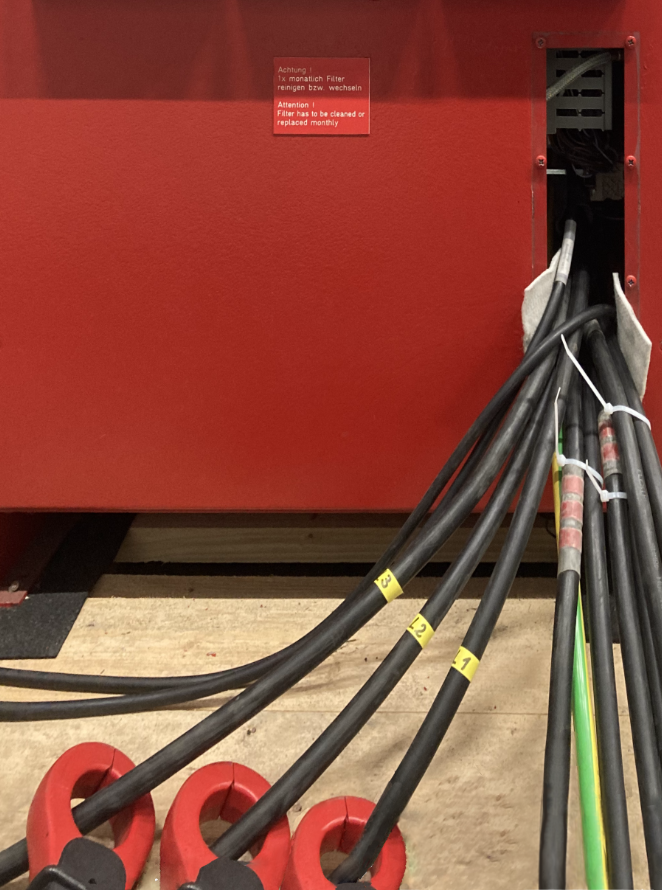
\includegraphics[height=5cm]{Bilder/Stromzangen.png}
         \caption{Stromzangen am Lastausgang}
         \label{fig:Umformer_Stromzangen}
     \end{subfigure}\hfill%
    \begin{subfigure}[t]{.4\textwidth}
          \centering
          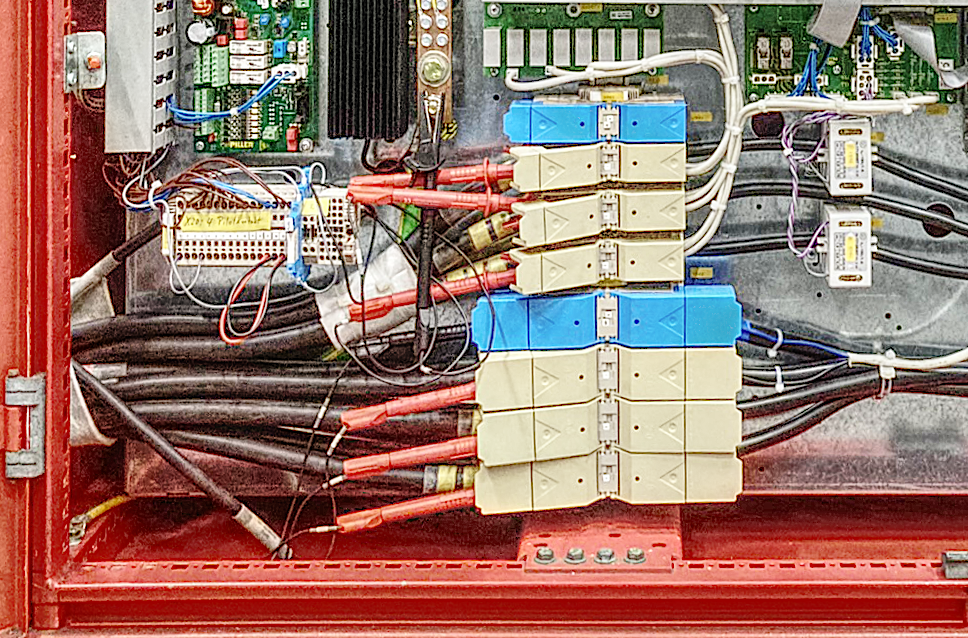
\includegraphics[height=5cm]{Bilder/Klemmen.png}
          \caption{Klemmen zur Spannungsmessung}
          \label{fig:Umformer_vorne}
     \end{subfigure}\hfill%
     \begin{subfigure}[t]{.2\textwidth}
          \centering
          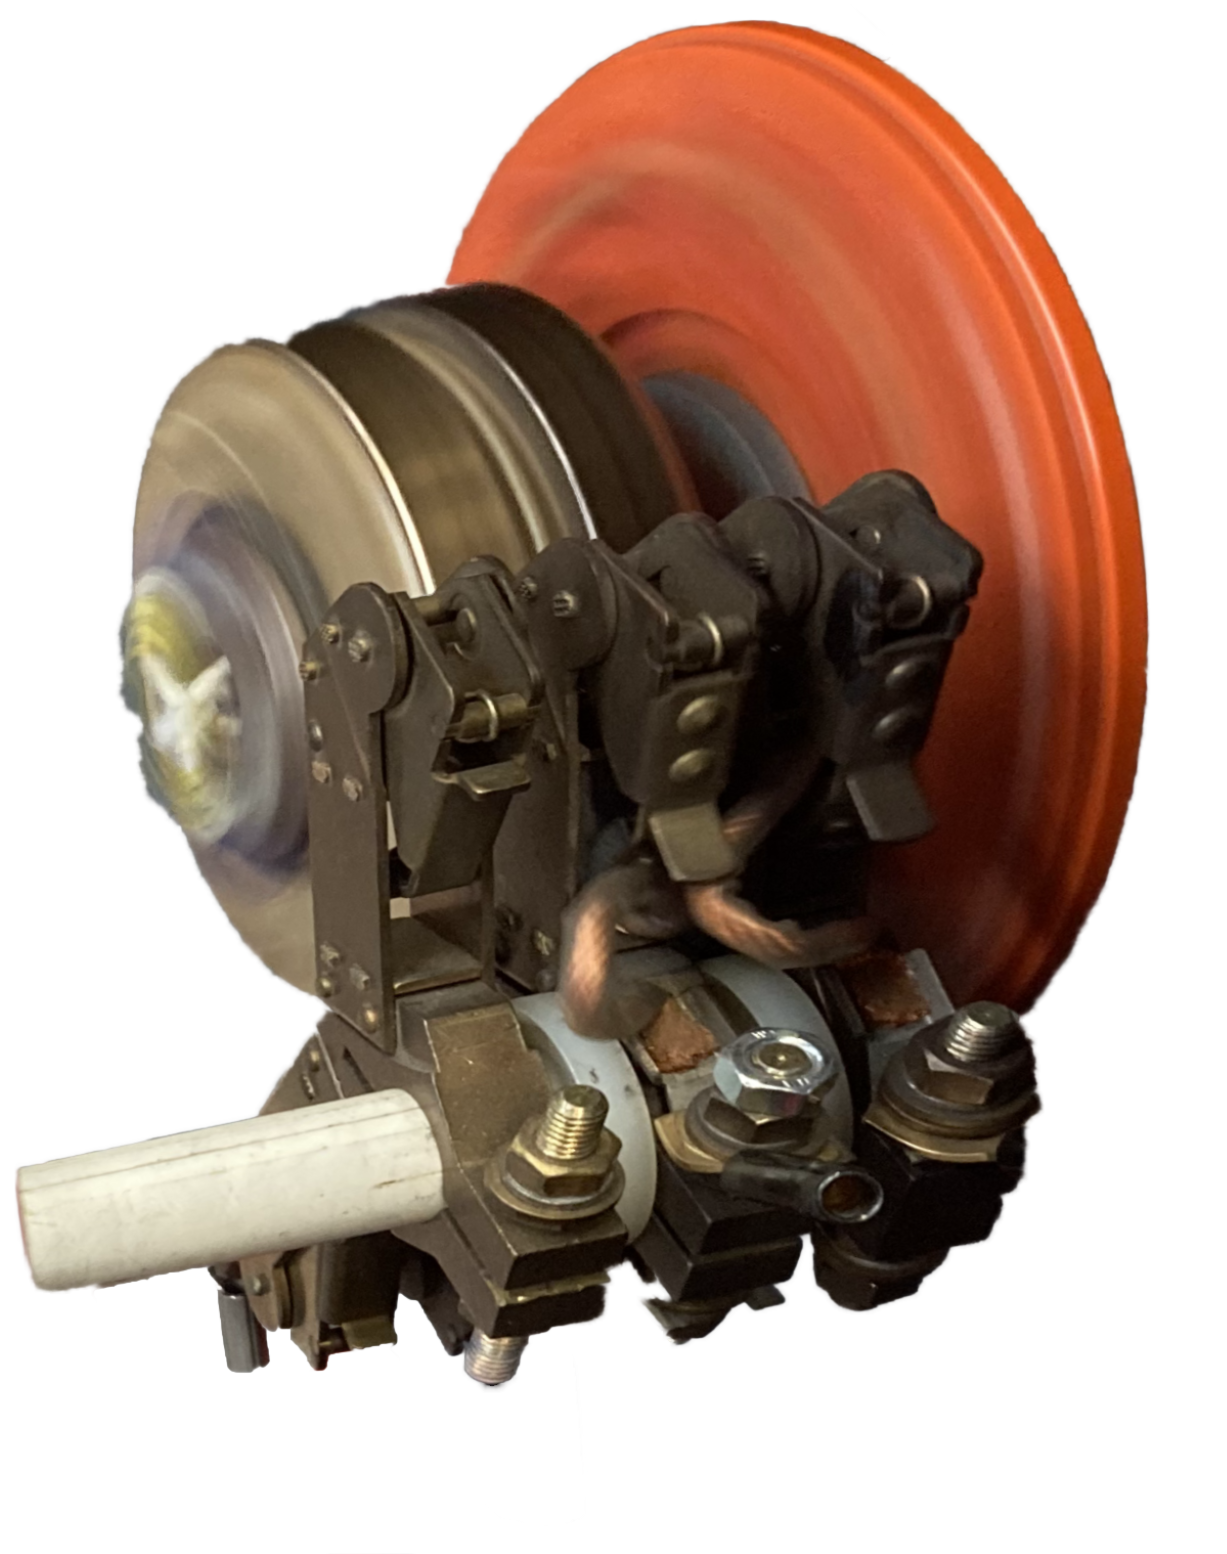
\includegraphics[]{Bilder/Polrad_freigestellt.png}
          \caption{Polrad}
          \label{fig:Umformer_Polrad}
     \end{subfigure}\hfill%
    \caption{Umformer mit Messanschlüssen}
    \label{fig:Messaufbau}
\end{figure}

Die aufgenommenen Messgrößen sind die drei Strom- und Spannungsphasen des Netzeingangs und des Ausgangs der Anlage, der Strom und Spannungsausgang am Spannungserzeuger des Reglers und die gleichgerichtete Spannung am Ausgang des auf dem Polrad mitrotierenden Gleichrichters (\emph{Polradspannnung}). Gefahren wurden drei Arten von Messläufen: \begin{enumerate}
    \item Statische Messung: Ein kurzer Zeitabschnitt der Messgrößen wurde mit den Lasten $[\unit[0]{\%}, \unit[25]{\%}, \unit[50]{\%}, \unit[75]{\%}, \unit[100]{\%}, \unit[125]{\%}, \unit[150]{\%}]$ der Nennscheinleistung jeweils bei einem Leistungsfaktor von $\mathrm{Pf} = 1$ und $\mathrm{Pf} = 0,8$ aufgenommen.Die Messung bei $\unit[0]{\%}$~Last fand jedoch nur bei $\mathrm{Pf}=1$ statt.
    \item Dynamische Messung: Die Messgrößen wurden für ca $\unit[10]{s}$ aufgezeichnet. Während der Messung wurde ein Lastsprung ausgeführt, für jeden Sprung jeweils ein Aufschalten und ein Abwurf der Last und ebenfalls jeweils mit einem Leistungsfaktor von $\mathrm{Pf}=1$ und $\mathrm{Pf}=0,8$. Vermessen wurden die Lastsprünge $[\unit[0]{\%}, \unit[50]{\%}]$, $[\unit[0]{\%}, \unit[100]{\%}]$ und $[\unit[50]{\%}, \unit[100]{\%}]$.
    \item Dynamische Messung mit Veränderung der Reglerparameter: Wie bei der Dynamischen Messung ohne Veränderung der Reglerparameter wurden die Messgrößen für ca $\unit[10]{s}$ während eines Lastsprungs aufgenommen, jedoch mit veränderten Reglerparametern. Die eingestellten Parameter können den \cref{tab:Parameter-D-Messung,tab:Parameter-I-Messung,tab:Parameter-P-Messung,tab:Parameter-PI-Messung} im \cref{sec:ReglerparameterDynamischeMessung} entnommen werden. Die Lastsprünge (Aufschalten und Abwurf) wurden bei $[\unit[50]{\%}, \unit[100]{\%}]$ Last und einem Leistungsfaktor von $\mathrm{Pf}=0,8$ ausgeführt.
\end{enumerate}

Die Ströme wurden mit Stromzangen (siehe \cref{fig:Umformer_Stromzangen}) an den Zu- und Ableitungen und die Ein- und Ausgangsspannungen, wie auch die Reglerspannung wurden mit entsprechenden Klemmen im Frequenzumformer aufgenommen (siehe \cref{fig:Umformer_vorne}). Die Polradspannung wurde über dafür montierte Schleifringe von der Welle abgeführt (\cref{fig:Umformer_Polrad}). Mit der Messsoftware wurden die Messdaten aufgezeichnet und wegen der höheren Schreibgeschwindigkeit in einem Binäformat abgespeichert. Für die weitere Verarbeitung wurden die Messwerte anschließend in das Textformt \texttt{.csv} umgewandelt. Die Aufzeichnung der transienten Größen erfolgte mit einer Abtastrate von $f_{\mathrm{s}}=\unit[60]{kHz}$.

\section{Aufbereitung der Messergebnisse}
\label{sec:Auswertung_Messeregbnisse}
Die Aufbereitung der Messergebnisse erfolgte in einem Jupyter-Notebook mit Python und einem ergänzenden Python-Modul \texttt{preprocessData.py}. Der entwickelte Quellcode ist im Anhang unter \cref{lst:PreprocessData} zu finden.

%Die Auswertung der Messergebnisse unterteilte sich in zwei Phasen: Zuerst mussten die Daten aufbereitet werden, Verläufe geglättet und Leistung, Frequenzen und Effektivwerte der elektrischen Größen bestimmt werden. Im nächsten Schritt konnten dann die Kenndaten der elektrischen Anlage und der einzelnen Maschinen gewonnen und zum Abgleich mit dem Modelica-Modell vorbereitet werden. 

Mit dem Modul wurden aus den eingelesenen Daten die folgenden Größen in dieser Reihenfolge bestimmt:
\begin{itemize}
    \item Leiter-Leiter-Spannungen aus den gemessenen Leiter-Neutralleiterspannungen: 
        \begin{equation}
        x_{\mathrm{LL}} = x_{\mathrm{2\,LN}} - x_{\mathrm{1\,LN}}
        \end{equation}
    \item Frequenzen der Größen: Da die betrachteten Strom- und Spannungsverläufe die Sinusform gut annähern, konnten die Periodenlängen bzw. Frequenzen durch Erkennen der Nulldurchgänge (\emph{Zero-Crossing}) ermittelt werden.
    \item Effektivwerte der Größen, ermittelt jeweils über eine Periode mit \begin{equation}
        X_{\mathrm{eff}}=\sqrt{\mathrm{mean}(x^2)},
    \end{equation}
    wobei $\mathrm{mean(x)}$ als der arithmetische Mittelwert gemäß \begin{equation}
        \mathrm{mean}(x) \coloneqq \frac{1}{n} \sum_{i=1}^n x_i
    \end{equation}
    definiert ist.
    \item Scheinleistung am Ein- und Ausgang, jeweils über eine Periode ermittelt nach \begin{equation}
        S_i = u_i \cdot i_i
    \end{equation}
    \item {Gleitender Mittelwert des Stroms und der Spannung am Ausgang des Reglers. Gemittelt wurde über 10 Perioden mit einer Frequenz von $f=\unit[2500]{Hz}$, die aus den Rohdaten für die Pulse abgelesen wurde.
    }
\end{itemize}
Anschließend wurden die Datenreihen jeweils über 10 Perioden mit einem gleitenden Mittelwert geglättet (bzw. über $\Delta T_{\mathrm{mittel}}=\frac{10}{\unit[2500]{Hz}}=\unit[4]{ms}$ im Falle der Reglerausgangsgrößen). Zur weiteren Auswertung wurden die Messgrößen als Spalten in einem Pandas-\texttt{Dataframe} angeordnet und, um Wartezeiten durch erneutes Einlesen der Daten zu vermeiden, als binäres Speicherabbild gesichert.
%TODO: Auf Zeitverläufe der Spannungen hinweisen

\chapter{Verifikation und Validierung}
\label{chap:VerfikationValidierung}
In diesem Kapitel soll das Maschinenmodell verifiziert und validiert werden. Die Verifikation verfolgt die Fragestellung, ob das Modell entsprechend der Systembeschreibung aus den Abschnitten \labelcref{sec:Uberblick,sec:gesamtsystem} implementiert wurde und die erwarteten Ergebnisse liefert. In der Validierung des Modells wird dann untersucht, in wie weit Modell und realer Umformer übereinstimmen und gegebenenfalls wird das Modell oder dessen Parametrierung an das Verhalten des realen Umformers angepasst. Verwendet werden dazu die in \cref{chap:Versuch} aufgenommenen Messdaten. 

In der Anwendung auf das Modell ist die Verifikation und Validierung ein ständiger Prozess, der die Modellierung begleitet und zu stetigen Anpassungen des Modells führt. Daher sollen hier nur die angewendeten Methoden und deren Ergebnisse in der zuletzt ausgeführten Modellversion angegeben werden, wobei berücksichtigt werden muss, dass eine absolute Fehlerfreiheit nicht mit überschaubarem Aufwand gewährleistet werden kann (vgl. \cite[S.~14ff.]{rabeVerifikationUndValidierung2008}).
 
\section{Verifikation}
\label{sec:Verifkation}
Die Verifikation des Modells kann aufgeteilt werden in die Verifikation der einzelnen verwendeten Teilmodelle und dem aus diesen Teilmodellen zusammengestellten Gesamtmodell. Die einzelnen Teilmodelle entstammen dabei, wie in \cref{chap:Modellierung} beschrieben, der MSL oder sind aus Komponenten der MSL aufgebaut. Diese Modelle können als plausibel angenommen werden, da die Implementierungen aus allgemein anerkannten Standardmodellen entspringen, deren Umsetzung durch ihre öffentliche Zugänglichkeit, Tests und Anpassungen kontrolliert wurde. Damit beschränkt sich die Untersuchung auf die Verifikation des Gesamtmodells, also der Auswahl und Verbindung der Teilmodelle. 

Entsprechend den Anforderungen an das Modell gehört zu den Hauptaufgaben des Modells die Simulation der übertragenen elektrischen Leistung und das Verhalten der Ausgangsspannung bei verschiedenen Parametrierungen. Die korrekte Funktionsweise des Spannungsreglers und damit die Wiedergabe der Ausgangsspannung kann direkt aus den Ergebnissen der Simulation eines Lastsprunges abgelesen werden. Einen solchen Zeitverlauf der Ausgangsspannung zeigt \cref{fig:Verifikation_Spannung}. Nach Einschalten des Reglers bei $t=\unit[0,7]{s}$ folgt der Effektivwert der Ausgangsspannung dem Sollwert und schwingt bis $t=\unit[2]{s}$ bei $U_{\mathrm{eff}}=\unit[115]{V}$ ein. Bei $t=\unit[2,2]{s}$ wird eine Lastaufschaltung ausgeführt. Der resultierende Spannungseinbruch wird durch den Spannungsregler bis $t\approx\unit[3]{s}$ ausgeregelt.
\begin{figure}
    \centering
    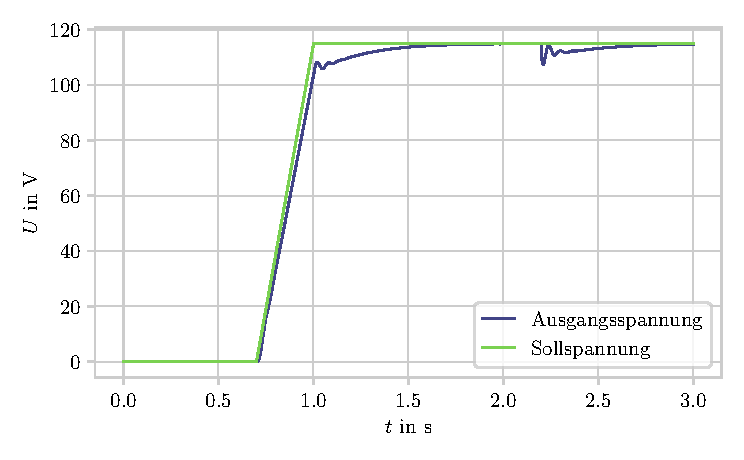
\includegraphics{Bilder/Verifikation_Spannung.pdf}
    \caption{Effektivwert der Ausgangsspannung (LN-Spannung) und Sollwert des Reglers}
    \label{fig:Verifikation_Spannung}
\end{figure}

Die Frequenz der Ausgangsspannung wird im Modell aus Geschwindigkeitsgründen aus der Winkelgeschwindigkeit der Welle und der Polpaarzahl des Synchrongenerators ermittelt. Um die Kopplung der Spannungsfrequenz mit der Winkelgeschwindigkeit der Welle zu überprüfen, wird die so ermittelte Frequenz mit der Frequenz der Zeitverläufe der drei Phasen der Ausgangsspannung verglichen. \cref{fig:Verifikation_Frequenz} zeigt den Verlauf der Frequenz, ermittelt durch Messen der Zeit zwischen den Nulldurchgängen (blaue Kurve) und die zum gleichen Zeitpunkt aus der Winkelgeschwindigkeit ermittelte Frequenz. Wie zu sehen ist, stimmen beide Kurven miteinander überein. Der Abweichung der Frequenz aus den Nulldurchgängen im Sprungmoment von der Frequenz aus der Winkelgeschwindigkeit erklärt sich aus Abweichungen der Spannung von der reinen Sinusform (Oberschwingungen) im Sprungmoment.
\begin{figure}
    \centering
    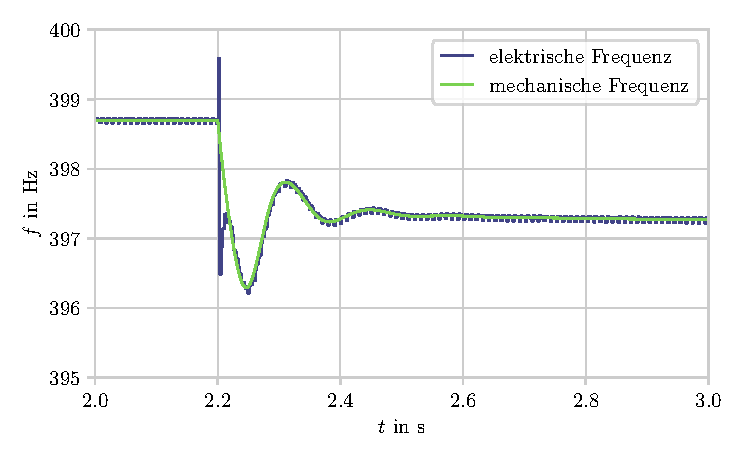
\includegraphics{Bilder/Verifikation_Frequenz.pdf}
    \caption{Frequenz der Ausgangsspannung, ermittelt aus der Zeit zwischen Nulldurchgängen und aus der Winkelgeschwindigkeit}
    \label{fig:Verifikation_Frequenz}
\end{figure}

Schließlich kann die Struktur des Modells und der Verbindungen mittels des Energie\-flusses zwischen den Teilmodellen überprüft werden. Die Übersicht in \cref{fig:Wirkungsgraph} gibt dazu die Referenz. \cref{fig:VerifikationLeistungen} zeigt Zeitverläufe verschiedener Leistungen an verschiedenen Punkten im Modell. Aus der Netzspannungsquelle wird elektrische Leistung vom Stator der Asynchronmaschine über den Luftspalt auf die Welle übertragen. Die Differenz zwischen den Leistungen ergibt sich aus den elektrischen Verlusten im Stator und im Rotor und aus den Verlusten im Luftspalt. Die mechanische Leistung teilt sich auf den Synchrongenerator und die Erregermaschine auf, wobei der Hauptteil von dem Generator aufgenommen wird. Die Erregermaschine erhält neben der mechanischen Leistung einen kleinen Beitrag aus der Erregung durch den Spannungsregler und gibt die erzeugte elektrische Leistung an den Synchrongenerator als Erregung ab. Der Synchrongenerator erzeugt dann aus der mechanischen Leistung elektrische Energie (ebenfalls verlustbehaftet), die an den Ausgang abgegeben wird. Mit Berücksichtigung der Verlustleistungen stimmen die Kurven miteinander überein, wobei beachtet werden muss, dass die Abweichungen im Sprungmoment von der Aufnahme oder Abgabe von Energie aus Speichern wie der rotatorischen Trägheit verursacht wird.
\begin{figure}
    \centering
    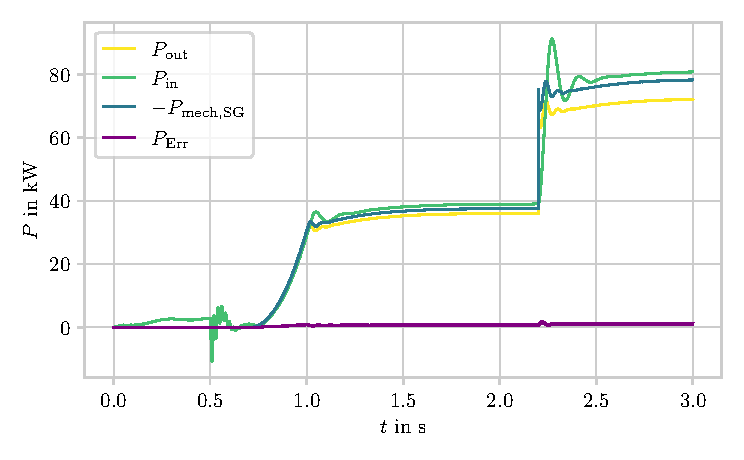
\includegraphics{Bilder/Verifikation_Leistung.pdf}
    \caption{Übersicht über die übertragenen Leistungen}
    \label{fig:VerifikationLeistungen}
\end{figure}

Damit können die wichtigsten Eigenschaften des Modells als plausibel betrachtet werden. Im nächsten Schritt wird dann untersucht, wie das Modell mit dem realen Umformer übereinstimmt.

\section{Validierung}
\label{sec:Validierung}
Die Validierung des Simulationsmodells hat zum Ziel, Übereinstimmung zwischen dem realen Verhalten der Anlage und dem Verhalten des Modells zu gewährleisten. Dabei muss berücksichtigt werden, dass jedes Übereinstimmen nur in bestimmten Grenzen möglich sein kann, da jedes Modell eine Vereinfachung der Realität darstellt. Die Validierung erfolgt durch Vergleich des Modellverhaltens mit den in \cref{chap:Versuch} aufgenommenen und aufbereiteten Messdaten. 

Das begründet eine zusätzliche Einschränkung der Möglichkeiten zur Validierung des Modells, da zum Einen jede Messung fehlerbehaftet ist und zum Anderen nur beschränkte Möglichkeiten zur Messung des Systems zur Verfügung standen. So war es nur möglich, die Polradspannung und die elektrischen Ein- und Ausgangsgrößen des Systems aufzunehmen. Messung der Zeitkonstanten oder Induktivitäten der elektrischen Maschinen konnten an der betrachteten Anlage nicht ohne erheblichen Aufwand durchgeführt werden, da die elektrischen Maschinen nicht einzeln zugänglich waren.

\paragraph{Drehzahl-Drehmoment-Kennlinie der ASM}
Die Drehzahl-Drehmoment-Kennlinie des Asynchronmotors beeinflusst das Verhalten der elektrischen Anlage bei Belastung: Je steiler (\emph{härter}) die Kennlinie des Motors ist, desto weniger stark wird der Motor verlangsamt durch Erhöhung des Lastmoments. Die Frequenz der Ausgangsspannung ändert sich also weniger bei Belastung der Maschine. Aus den Messdaten kann die Kennlinie mit Hilfe der Ein- und Ausgangsleistungen und der Frequenz der Ausgangsspannung gewonnen werden. Die Winkelgeschwindigkeit der Welle ist nach \cref{eq:Winkelgeschwindigkeit-Frequenz} 
\begin{equation}
    \omega_{\mathrm{mech}} = \frac{2\pi}{f_{\mathrm{out}}} \label{eq:Winkelgeschwindigkeit-Frequenz}
\end{equation}
über die Polpaarzahl mit der Spannungsfrequenz verknüpft. Mit Kenntnis der Winkelgeschwindigkeit kann das maximale bzw. minimale Drehmoment, das über die Welle übertragen wird, aus den Leistungen nach \cref{eq:Moment-ASM} bestimmt werden.
\begin{equation}
    \frac{P_{\mathrm{out}} - P_{\mathrm{Regler}}}{\omega_{\mathrm{mech}}} < M_{\mathrm{ASM}} < \frac{P_{\mathrm{in}}}{\omega_{\mathrm{mech}}} \label{eq:Moment-ASM}
\end{equation}

Die Kennlinie des Simulationsmodells der ASM wird mit Hilfe einer separaten Simulation erzeugt. Die Winkelgeschwindigkeit der ASM wird über eine Rampenfunktion vorgegeben. Über einen Zeitraum von $\unit[10]{s}$ wird die Winkelgeschwindigkeit von $\omega_{\mathrm{mech}}=\unit[305]{\frac{rad}{s}}$ auf $\unit[315]{\frac{rad}{s}}$ erhöht (das entspricht dem Arbeitsbereich der ASM), sodass die Änderungen quasi-stationär stattfinden.
Damit ergibt sich die Drehzahl-Drehmoment-Kennlinie der ASM in \cref{fig:Validierung-ASMKennlinie}. Das Anpassen der simulierten Kennlinie an die Messdaten erfolgte durch Einstellen des Rotorwiderstands der ASM. Auch ein Abgleich anderer Größen der ASM wäre möglich gewesen. Jedoch lässt sich die Änderung der Kennlinie dann nicht eindeutig einer einzigen Variablen zuordnen, wodurch die Komplexität dieses Einstellverfahrens deutlich erhöht wird.
\begin{figure}
    \centering
    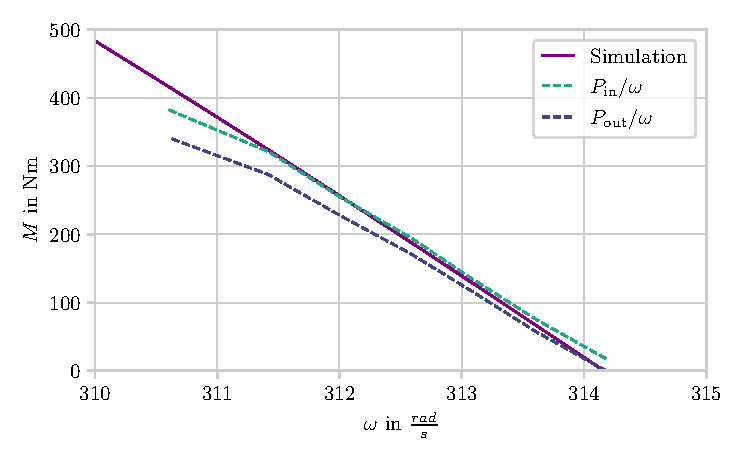
\includegraphics{Bilder/Validierung_Kennlinie.pdf}
    \caption{Drehzahl-Drehmomentkennlinie der Asynchronmaschine aus der Simulation und der Messung}
    \label{fig:Validierung-ASMKennlinie}
\end{figure}

\paragraph{Spannungskennlinie der Erregermaschine}
\begin{figure}[h!]
    \centering
    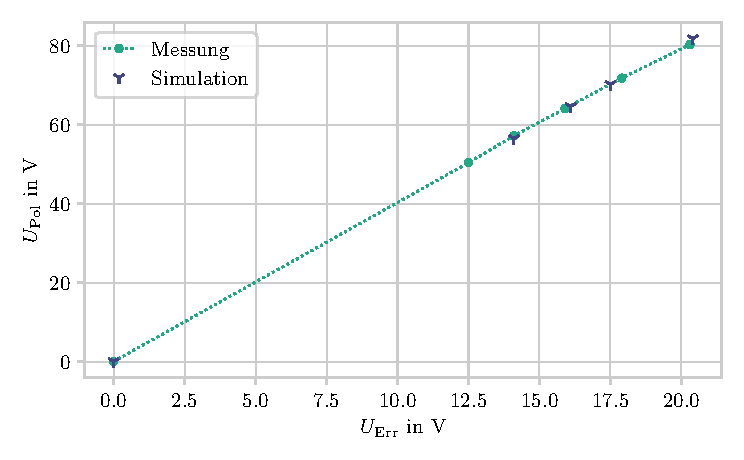
\includegraphics{Bilder/Validierung_Erregermaschine.pdf}
    \caption{Spannungkennlinie der Erregermaschine}
    \label{fig:Validierung-Erregermaschine}
\end{figure}
Die Spannungskennlinie der Erregermaschine beschreibt den Zusammenhang zwischen der Stellgröße des Reglers (der Erregerspannung) und der damit eingestellten gleichgerichteten Polradspannung zur Erregung des Synchrongenerators. Über die Impedanz des Synchrongenerators stellt sich durch die Polradspannung der Erregerstrom ein, der bei der hier betrachteten Maschine über die Schleifringe nicht gemessen werden konnte. Der Abgleich der Spannungskennlinie mit den Messdaten erfolgte durch Aufbringen verschiedener Lastsprünge in der Simulation und anpassen der Erregerwiderstände der Erregermaschine und des Synchrongenerators. Die resultierende Spannungskennlinie zeigt \cref{fig:Validierung-Erregermaschine}.

\paragraph{Verschiedene Lastsprünge}
Die Simulationsergebnisse des angepassten Modells werden mit der Messung verglichen. Betrachtet wird die Ausgangsspannung bei Ausführen verschiedener Lastsprünge mit $\mathrm{Pf}=0,8$. Dieser Leistungsfaktor wird gewählt, da hier die Spannungsamplituden im Sprungmoment größer sind als bei $\mathrm{Pf}=1$ (vgl. \cref{fig:ZeitverlaufDynamischOhneRegleraenderung}). Aus dem Vergleich der Simulationseregbnisse mit den Messergebnissen kann der Modellierungsfehler bestimmt werden. Quantifiziert wird der Fehler mit der \emph{Wurzel des mittleren quadratischen Fehlers} (\emph{\textbf{R}oot \textbf{M}ean \textbf{S}quare \textbf{E}rror} -- RMSE). \begin{equation}
\mathrm{RMSE} = \mathrm{mean}\left(\left| \hat{y} - y \right|\right).
\end{equation}
Neben dem RMSE könnte nach \cite{pontiusComponentsInformationMultiple2008} auch die \emph{mittlere absolute Abweichung} (\textbf{M}ean \textbf{A}bsolute \textbf{E}rror -- MAE) betrachtet werden. Der RMSE bewertet im Gegensatz zum MAE kurze große Abweichungen stärker als lange geringe Abweichungen und wird hier bevorzugt, da Differenzen zwischen Simulation und Messung vorrangig während des Lastsprungs auftreten.

\cref{fig:ValSpannung} zeigt die gemessenen und simulierten Spannungen bei verschiedenen Lastsprunggrößen. Die simulierten Spannungen stimmen gut mit den Messungen überein. Der schlechteste RMSE beträgt \unit[1,33]{V}. Mit einer Spannungsamplitude von $\Delta U\approx\unit[16]{V}$ ergibt das eine Abweichung von ca \unit[8,3]{\%}. Weiterhin zeigt sich, dass  die Lastsprünge mit kleinerer Amplitude auch mit einem kleineren Fehler behaftet sind. Der kleinste Fehler tritt im Lastbereich von \unit[50]{\%} bis \unit[100]{\%} auf. Der größte Unterschied zwischen Messung und Simulation zeigt sich im Abklingverhalten nach dem Sprung. In allen untersuchten Fällen stellt sich in der Simulation der stationäre Zustand langsamer ein als in der Messung. Das Abklingverhalten eines RL-Schwingkreis wird mit einer Zeitkonstante $T=\frac{L}{R}$ beschrieben. Da die Widerstände der beiden Synchrongeneratoren oben bereits abgeglichen wurden, könnte die Abklingzeit durch Variation der Induktivitäten angepasst werden. Eine Variation der Induktivitäten wird im Folgenden Abschnitt durchgeführt.
\begin{figure}
\centering
\begin{subfigure}{.49\textwidth}
	\centering
	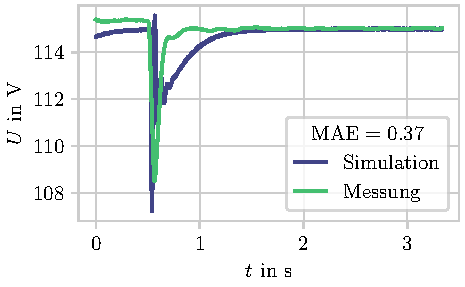
\includegraphics[]{Bilder/ValMessung_0-50.pdf}
	\caption{Lastsprung \unit[0]{\%}-\unit[50]{\%}}
	\label{fig:ValMessung0-50}
\end{subfigure}
\begin{subfigure}{.49\textwidth}
	\centering
	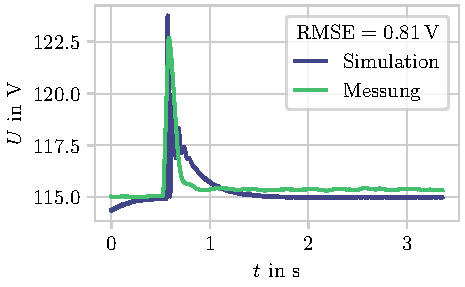
\includegraphics[]{Bilder/ValMessung_50-0.pdf}
	\caption{Lastsprung \unit[50]{\%}-\unit[0]{\%}}
	\label{fig:ValMessung50-0}
\end{subfigure}
\begin{subfigure}{.49\textwidth}
	\centering
	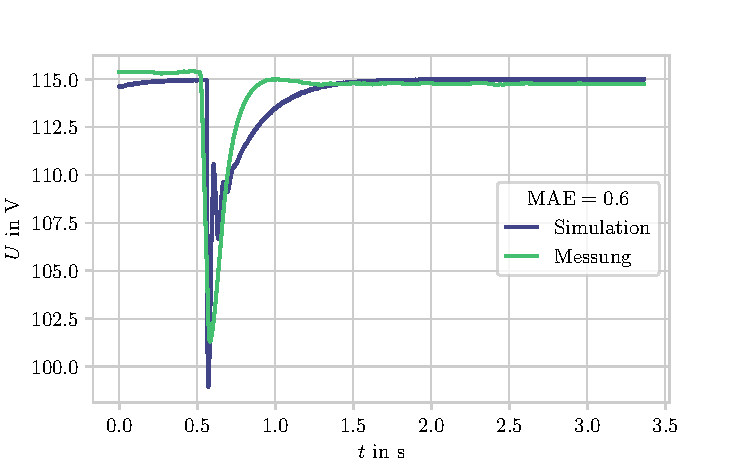
\includegraphics[]{Bilder/ValMessung_0-100.pdf}
	\caption{Lastsprung \unit[0]{\%}-\unit[100]{\%}}
	\label{fig:ValMessung0-100}
\end{subfigure}
\begin{subfigure}{.49\textwidth}
	\centering
	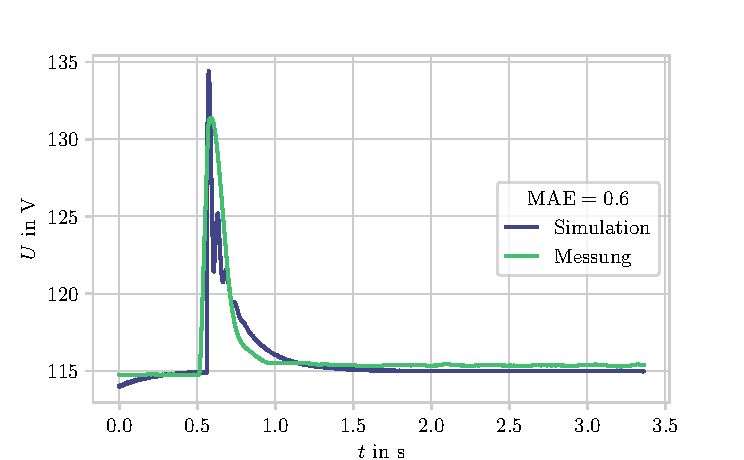
\includegraphics[]{Bilder/ValMessung_100-0.pdf}
	\caption{Lastsprung \unit[100]{\%}-\unit[0]{\%}}
	\label{fig:ValMessung100-0}
\end{subfigure}
\begin{subfigure}{.49\textwidth}
	\centering
	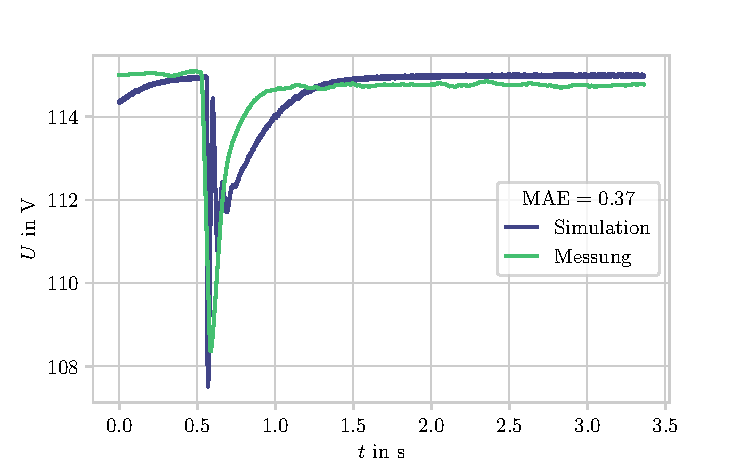
\includegraphics[]{Bilder/ValMessung_50-100.pdf}
	\caption{Lastsprung \unit[50]{\%}-\unit[100]{\%}}
	\label{fig:ValMessung50-100}
\end{subfigure}
\begin{subfigure}{.49\textwidth}
	\centering
	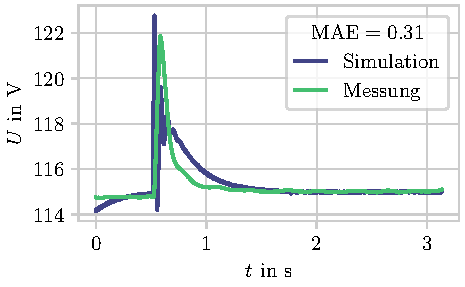
\includegraphics[]{Bilder/ValMessung_100-50.pdf}
	\caption{Lastsprung \unit[100]{\%}-\unit[50]{\%}}
	\label{fig:ValMessung100-50}
\end{subfigure}
\caption{Gemessene und simulierte Ausgangsspannungen bei verschiedenen Lastsprüngen}
\label{fig:ValSpannung}
\end{figure}
\chapter{Parameterstudie zum Einfluss der Induktivitäten und Reglerparameter}
\label{chap:Auswertung}
Dieses Kapitel beschreibt \emph{eine} beispielhafte Anwendung des Frequenzumformermodells. Es soll mittels eines Parameterstudie untersucht werden, wie groß der Einfluss der Veränderung der Parameter der elektrischen Maschinen im Vergleich zu einer Veränderung der Reglerparameter auf das dynamische Verhalten der Anlage ist. Neben weiteren Möglichkeiten zur Auswertung des Modells (beispielsweise Systemidentifikation der Regelstrecke oder Optimierung der Maschinen- und Reglerparameter) ist aufgrund des objektorientierten und akausalen Modellierungsprinizps auch eine Einbettung des Modells in übergeordnete Modelle (z.B. zur Simulation von Verbänden mehrerer Anlagen) oder auch eine Umkehr der Kausalität (z.B. Untersuchung der Rückspeisefähigkeit, Umkehrung der Regelstrecke zum Reglerentwurf) denkbar.

\section{Problemstellung}
\label{sec:ProblemstellungParameterSweep}
Das hier untersuchte Problem entspringt der Fragestellung, ob sich das dynamische Verhalten der Anlage eher durch Optimieren des Reglers verbessern lässt oder eine Verbesserung nur durch Änderung der elektrischen Parameter möglich ist. Dieser zweite Fall wird zutreffen, falls der Regler bereits optimal eingestellt ist. 

Gleichzeitig bietet die Parameterstudie auch die Möglichkeit zu untersuchen, wie die Qualität der Modellparametrierung weiter verbessert werden kann. Einige Widerstände der elektrischen Maschinen wurden bereits in \cref{chap:VerfikationValidierung} mit Hilfe der Messungen angepasst. Untersuchungen zum Abgleich der Induktivitäten der Maschinen konnten jedoch nicht durchgeführt werden. Die Parameterstudie bietet daher die Möglichkeit, zu untersuchen, welche Größen der Maschinen großen Einfluss auf das dynamische Verhalten haben und in welchen Wertebereichen eine Annäherung an die Messergebnisse erzielt werden kann.

Bewertet wird das dynamische Verhalten mit dem Integral über das Fehlerquadrat (\emph{\textbf{I}ntegrated \textbf{S}quared \textbf{E}rror} -- ISE), wobei der Fehler die Differenz zwischen der Ausgangsspannung und dem Sollwert bei einem Lastsprung ist, siehe \cref{eq:ISE}. Der ISE berücksichtigt durch das Quadrat große Abweichungen durch Schwingen stärker als andere Integralkriterien und wird in der Literatur auch als Standard zur Reglereinstellung angegeben (\cite[S.~190]{unbehauenRegelungstechnikKlassischeVerfahren2008}).
\begin{equation}
    \label{eq:ISE}
    \mathrm{ISE} = \int_0^T (115-y(t))^2 \mathrm{d}t
\end{equation}

\section{Durchführung}
In der Parameterstudie werden die Werte der elf Induktivitäten der elektrischen Maschinen einzeln variiert und ihre Auswirkung auf den ISE untersucht, wobei beachtet werden muss, dass bei der Auswahl der Parameter die reale Umsetzbarkeit \emph{nicht} berücksichtigt wurde. Für jeden Parameter werden 120 Variationen simuliert, jeweils 60 Punkte für eine Vergrößerung und 60 Punkte für eine Verkleinerung des Nennwertes. Die Verteilung der Änderung des Nennwerts wird durch eine Exponentialfunktion so beschrieben, dass der 30. Schritt den Nennwert um den Faktor 2 (also auf 50\% bzw. 200\%) ändert. Die exponentielle Verteilung wird gewählt, da sie über die festgelegte Zahl der Schritte eine Änderung der Parameter in weitem Bereich ermöglicht: Im Bereich bis zum 30. Schritt werden die Parameter nur moderat variiert, ähnlich einer linearen Verteilung, ab dem 30. Schritt jedoch ist die Änderung durch die exponentielle Verteilung größer als die der linearen Verteilung. Die Werte nähern sich einer quadratischen Verteilung an (siehe \cref{fig:VerteilungParameter}).
\begin{figure}
    \centering
    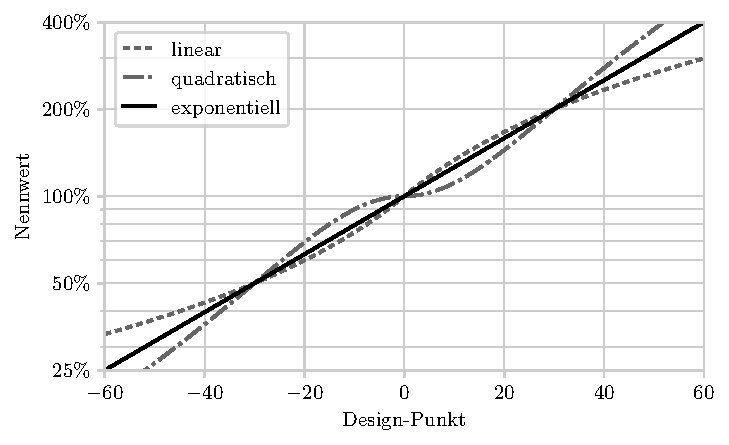
\includegraphics[width=.8\textwidth]{Bilder/verteilung_log.pdf}
    \caption{Verschiedene Verteilungsfunktionen zur Parametervariation}
    \label{fig:VerteilungParameter}
\end{figure}

Durchgeführt wird die Parameterstudie mit Hilfe eines Python-Skripts (siehe \cref{lst:ModelicaSweep}). Das kompilierte Modell des Frequenzumformers wird mit dem Skript gestartet und der geänderte Parameter zugewiesen. Anschließend werden die Simulationsergebnisse in Python eingelesen und der ISE (vgl. \cref{eq:ISE}) vom Sprungbeginn an  über ein Intervall von $T=\unit[0,8]{s}$ berechnet, bis die Ausgangsspannung (bei Nennparametern) den stationären Zustand erreicht. Zusätzlich zu der Parameterstudie über die Induktivitäten der elektrischen Maschinen wurde auch eine Parameterstudie mit veränderten Reglerparametern wie in der dynamischen Messung in \cref{sec:Messaufbau} durchgeführt.

\section{Ergebnisse}
Die aus der Parameterstudie der Induktivitäten resultierenden Zeitverläufe der Spannungen zeigen \cref{fig:InduktivitatenSweepA,fig:InduktivitatenSweepB}. Die Spannungsverläufe aus der Studie der Reglerparameter zeigt \cref{fig:SpannungenReglerSweep}.

Die Zeitverläufe der Spannungen geben einen Überblick über den Einfluss der einzelnen Induktivitäten auf das dynamische Verhalten. So ist zu erkennen, dass die Induktivitäten der Asynchronmaschine generell kaum Einfluss nehmen auf die Spannungsverläufe. Ebenso ist auch der Einfluss der Induktivitäten bezüglich der q-Achse generell geringer als derjenige der entsprechenden Induktivität bezüglich der d-Achse. Den größten Einfluss auf den Spannungsverlauf haben demnach die Hauptinduktivitäten $L_{\mathrm{md}}$ der beiden Synchronmaschinen, die bei großen Minderungen der Induktivitäten einen stationären Regelfehler aufweisen.

Die Einflüsse der weiteren Induktivitäten der beiden Synchronmaschinen sind wesentlich geringer und verteilen sich auf unterschiedliche Weise, wobei auch beachtet werden muss, dass die Rotorstreuinduktivitäten $L_{\mathrm{r\sigma}}$ bei der Erregermaschine nicht auftreten, da diese ohne Dämpferkäfig ausgeführt ist. Nach der Hauptinduktivität bezüglich der d-Achse haben bei dem Synchrongenerator die Streuinduktivität des Stators und die Streuinduktivität des Rotors bezüglich der d-Achse den größten Einfluss auf das dynamische Verhalten, bei der Erregermaschine hingegen ist der Einfluss der Hauptinduktivität bezüglich der q-Achse etwas größer als der Einfluss der Streuinduktivität, wobei der unterschied sich vor Allem in der Dämpfung und der Frequenz des Schwingungsanteils zeigt. 

Ein Vergleich mit dem gemessenen Spannungsverlauf \cref{fig:ZeitverlaufDynamischOhneRegleraenderung} zeigt eine Annäherung der Simulation an die Messung bei moderater Verringerung der Hauptinduktivitäten bezüglich der d-Achse der beiden Synchronmaschinen.

\begin{figure}
    \captionsetup[subfigure]{aboveskip=1pt,belowskip=1pt}
    \centering
    \begin{subfigure}{\textwidth}
        \centering
        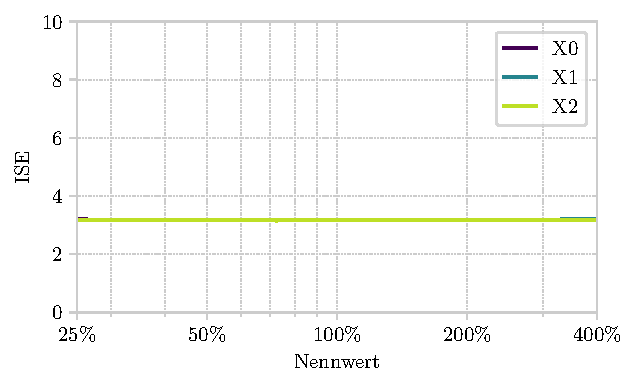
\includegraphics{Bilder/aimc_ISE.pdf}
        \caption{ASM}
        \label{fig:ISE_ASM}
    \end{subfigure}
    \begin{subfigure}{\textwidth}
        \centering
        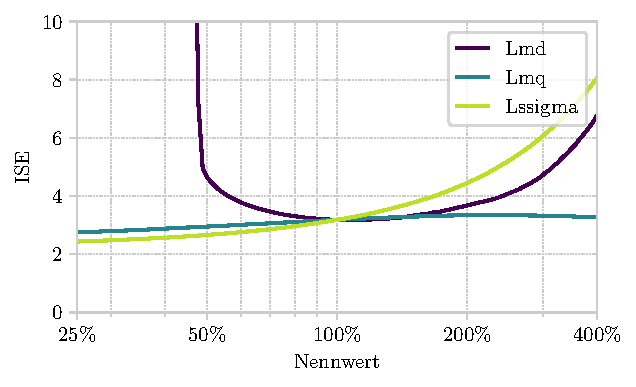
\includegraphics{Bilder/smee_ISE.pdf}
        \caption{Synchrongenerator}
        \label{fig:ISE_SG}    
    \end{subfigure}
%     \caption{Einfluss der Induktivitäten auf den ISE}
% \end{figure}
% \begin{figure}\ContinuedFloat
%     \centering
    \begin{subfigure}{\textwidth}
        \centering
        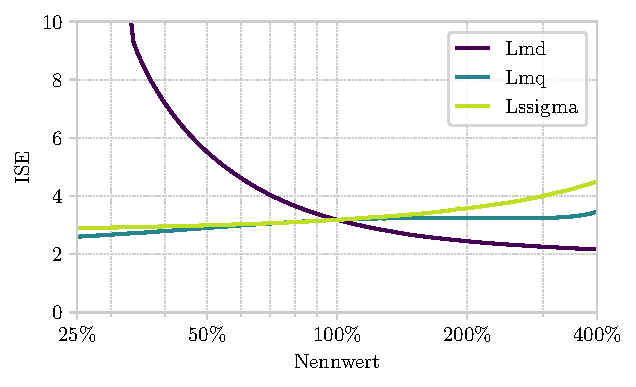
\includegraphics{Bilder/sM_E_ISE.pdf}
        \caption{Erregermaschine }
        \label{fig:ISE_ERR}    
    \end{subfigure}
    \caption{Einfluss der Induktivitäten auf den ISE}
\end{figure}
\begin{figure}
    \centering
    \begin{subfigure}{.49\linewidth}
        \centering
        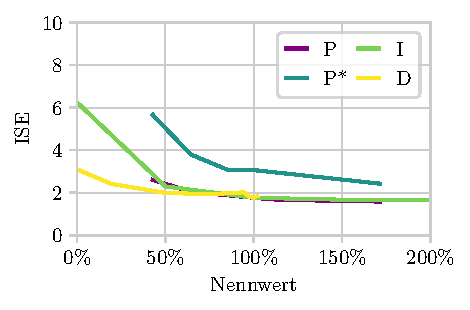
\includegraphics{Bilder/regler_ISE.pdf}    
        \subcaption{Messung}
    \end{subfigure}
    \begin{subfigure}{.49\linewidth}
        \centering
        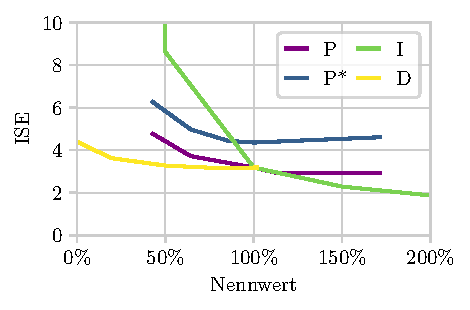
\includegraphics{Bilder/simulation_reglerSweep.pdf}
        \subcaption{Simulation}
    \end{subfigure}
    \caption{Einfluss der Reglerparameter auf den ISE}
    \label{fig:ISE_ReglerSweep}
\end{figure}

Der Einfluss der Induktivitäten und der Reglerparameter auf das dynamische Verhalten kann auch aus dem resultierenden ISE abgelesen werden. Die \cref{fig:ISE_ASM,fig:ISE_ERR,fig:ISE_SG} zeigen den Verlauf des ISE bei Veränderung der Induktivitäten. Der große Einfluss der Hauptinduktivitäten $L_{\mathrm{md}}$ der Synchronmaschinen zeigt sich im Verlauf des ISE. Der Knick im Verlauf des ISE bei ca \unit[50]{\%} bzw. \unit[33]{\%} des Nennwerts lässt sich begründen mit der beobachteten stationären Abweichung der Spannungen. Alle Verringerungen des ISE hingegen sind von kleinem Ausmaß.

Bei der Bewertung dieser stationären Abweichungen muss berücksichtigt werden, dass diese durch den Begrenzer des Spannungsreglers hervorgerufen wird, der einer Parametrierungsunsicherheit unterliegt. Die Reglerparameter sind gesichert, jedoch unterliegt die Umwandlung der reglerinternen Stellgröße auf die Ausgangsspannung einer unsicheren Datenlage. So kann die maximal mögliche Stellspannung um den Faktor 1,25 bis 1,5 nach oben abweichen, in Abhängigkeit von der gewählten maximalen Stellspannung (siehe \cref{sec:AbbildungReglerZahlen}. Mit einer größeren maximal möglichen Stellspannung würde auch der stationäre Regelfehler kleiner werden. Solange der Spannungsregler jedoch nicht bis zum Begrenzer aussteuert, beeinflusst dieser Fehler das dynamische Verhalten kaum.

Zum Vergleich der aus der dynamischen Messung mit Reglerveränderung erhaltenen Ergebnisse mit dem Simulationsmodell, wurden die entsprechenden Messparameter ebenfalls in der Simulation untersucht, mit derselben Methode wie bei den Induktivitäten (siehe \cref{fig:ISE_ReglerSweep,}). Der absolute Unterschied des ISE zwischen Simulation und Messung erklärt sich aus dem verbliebenen Modellierungs- und Parametrierungsfehler des Simulationsmodell. Es zeigt sich aber, dass das Trendverhalten der Reglerparameter in Simulation und Messung ähnlich sind. Die geringen Verminderungen des ISE (vor Allem in der Messung) zeigen, dass der Regler bereits gut, das heißt nahe eines lokalen Minimums des ISE eingestellt ist. Zum Nachweis des globalen Minimums wären weitere Untersuchungen hinsichtlich der Konvexität des Minimierungsproblems notwendig (siehe dazu \cite{eschVerfahrenZurGuteoptimalen2016}).

Den größten Einfluss auf den ISE nimmt die Verstärkung des I-Anteils. Generell bewirkt der I-Anteil des PID-Reglers stationäre Genauigkeit. Wird die Verstärkung des I-Anteils verringert, kann der Regler nicht mehr oder nicht in demselben Zeitraum den Regelfehler ausgleichen. Ähnlich wie bei den Hauptinduktivitäten der Synchronmaschinen zeigt sich sich diese bleibende Abweichung in dem hohen ISE. Der hohe Einfluss des P-Anteils ($P^*$) erklärt sich aus dem höheren Fehler im unveränderten Zustand durch den fehlenden D-Anteil (Konfiguration als PI-Regler). Wird dieser Startfehler berücksichtigt (vertikales Verschieben der Kurve), zeigt sich ein ähnliches Verhalten, wie bei Konfiguration als PID-Regler. Der Einfluss des P-Anteils und des D-Anteils fällt im Vergleich zum I-Anteil geringer aus, wobei der P-Anteil größeren Einfluss nimmt als der D-Anteil.

Zum Vergleich des Einflusses der Reglerparameter mit dem Einfluss der Induktivitäten auf den ISE wird die prozentuale Änderung des ISE bei Änderung eines Parameters um den Faktor 2 untersucht, das heißt in den Bereichen $[\unit[50]{\%},\unit[100]{\%}]$ und $[\unit[100]{\%},\unit[200]{\%}]$ des Nennwerts. Da die Reglerparameter nicht alle bis \unit[200]{\%} variiert wurden, werden die Verläufe des $P$-, $P^*$- und $I$-Anteils linear extrapoliert. Der ISE des $D$-Anteils hingegen wird nur im Intervall $[\unit[50]{\%},\unit[100]{\%}]$ ausgewertet, da im $[\unit[100]{\%},\unit[200]{\%}]$ Intervall zu wenig Parameter untersucht wurden. Berechnet wird die prozentuale Änderung des ISE mit Hilfe des Skripts in \cref{lst:Trendanalyse,lst:TrendanalyseCommand}. Die Ergebnisse aus Simulation und Messung für die Induktivitäten und die Reglerparameter sind in \cref{fig:trend_manager_scatter} dargestellt.
\begin{figure}
    \centering
    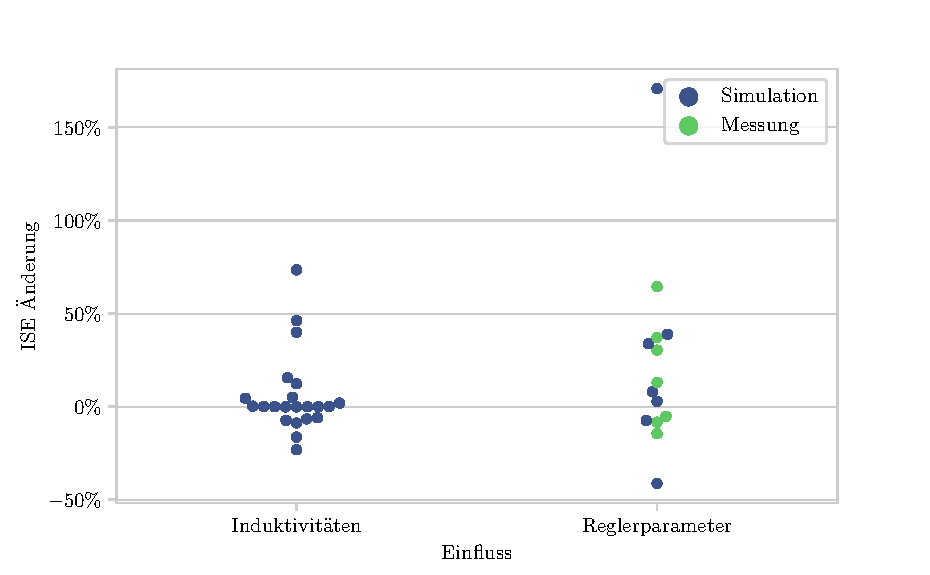
\includegraphics{Bilder/trend_manager_scatter.pdf}
    \caption{Prozentuale Änderung des ISE bei Variation um Faktor 2}
    \label{fig:trend_manager_scatter}
\end{figure}

Es zeigt sich, dass in dem untersuchten Parameterbereich die Induktivitäten und die Reglerparameter einen ähnlich großen Einfluss auf den ISE nehmen. Minimierung des ISE (d.h. Verbesserung des dynamischen Verhaltens) ist sowohl durch Variation der Induktivitäten als auch der Reglerparameter möglich. Das Potential zur Minimierung des ISE ist kleiner als das zur Vergrößerung. Das bedeutet, dass die aktuelle Parametrierung des Frequenzumformers sich nahe eines (zumindest lokalen) Minimums befindet. Die Parameter der Simulation weisen größeres Potential zur Verbesserung auf als die Messung, was durch den Modellierungsfehler erklärt wird. 

Diese Erkenntnisse können in der Auslegung und Regelung angewendet werden. Zunächst kann festgestellt werden, dass sowohl der Einfluss der Maschinenparameter als auch der der Reglerparameter im Entwurf berücksichtigt werden sollte, da beide ähnlich großen Einfluss auf das dynamische Verhalten nehmen. Dann ist aber auch offensichtlich, dass die beliebige Änderung der Reglerparameter mit vernachlässigbaren Kosten einhergeht, während eine Änderung der Induktivitäten nicht in beliebigem Rahmen möglich ist und mit hohen Entwicklungs- und Materialkosten verbunden ist. Daher empfiehlt es sich, zur Optimierung zuerst das Potential der Reglerparameter auszuschöpfen. Schlussendlich ergibt sich die Möglichkeit, Materialeinsparungen an den elektrischen Maschinen durch Erhöhung des ISE zu erkaufen und die Erhöhung durch Optimierung der Reglerparameter auszugleichen und trotzdem ein gutes (d.h. die Anforderungen erfüllendes) dynamisches Verhalten zu erzielen.

%% Trendanalyse mit Steigung:
% Zum Vergleich des Einflusses der Reglerparameter mit dem Einfluss der Induktivitäten auf den ISE wird die durchschnittliche Steigung des ISE in den Bereichen $[\unit[50]{\%},\unit[100]{\%}]$ und $[\unit[100]{\%},\unit[200]{\%}]$ des Nennwerts untersucht. Die durchschnittliche Steigung über einem Intervall ergibt sich nach \cref{eq:mittlereSteigung} aus dem Differenzenquotient der Intervallgrenzen. 
% \begin{equation}
%     \label{eq:mittlereSteigung}
%     \Bar{m} = \frac{1}{T} \int_{t_0}^{t_0+T} f'(t) \mathrm{d}t = \frac{f(t_0+T) - f(t_0)}{T}
% \end{equation}
% Berechnet wird die durchschnittliche Steigung für den ISE der Parameter mit Hilfe des Skripts in \cref{lst:Trendanalyse,lst:TrendanalyseCommand}. Die Ergebnisse aus Simulation und Messung für die Induktivitäten und die Reglerparameter zeigt \cref{fig:trend_manager_scatter}.
\chapter{Zusammenfassung und Ausblick}
\label{chap:ZusammenfassungAusblick}
%TODO: Zusammenfassung schreiben



%Notizen:
% Ergebnisse dieser Arbeit: In dieser Arbeit wurde
% - konnte ein objektorientiertes Modelle eines rotierenden Frequenzumformers hergelietet werden
% - Das Modell wurde mit Werten aus der Auslegung der Anlage parametriert. Wichtige Gleichungen zum Umformen der Auslegungsparameter wurden im Modell implementiert
% - Es wurden Eckpunkte zur Verifizierung & Validierung des Modells mittels Messergebnissen eines realen Umformers hergeleitet:
% 	- Das Gesamtmodell wird verifiziert, indem untersucht wird, ob das simulierte Verhalten den Erwartungen entspricht. Folgt die geregelte Spannung dem Sollwert, so kann geschlossen werden, dass der Regelkreis korrekt implementiert ist. Über die Untersuchung der Spannungsfrequenz am Ausgang der Anlage kann die Kopplung und Parametrierung der elektrischen Maschinen überprüft werden. Die Untersuchung der Leistungsflüsse im Modell und der Vergleich mit der Theorie stellt sicher, dass der Energieerhaltungssatz eingehalten wird und die Wirkrichtung der untersuchten Größen der Theorie folgt.
% 	- In der Validierung des Modells zeigt sich, ob die Anlage korrekt und hinreichend genau modelliert wurde. Über gemessene Kennlinien der elktrischen Maschinen kann die Parametrierung der Maschinen abgelglichen werden. --> Evtl. in V&V vgl. mit Messung hinzufügen!!!
% - Es wurden Parameterstudien zum Einfluss der Induktivitäten und Reglerparameter auf das dynamische Verhalten der Maschinen durchgeführt und das Potential zur Optimierung bestimmt. Es hat sich gezeigt, dass die Parametrierung der betrachteten Maschine nahe eines lokalen Minimums befindet. An dieser Stelle ist der Einfluss der beiden Parameterklassen ähnlich groß. Von den Induktivitäten beeinflussen hauptsächlich die Parameter der beiden Synchrongeneratoren das dynamische Verhalten. 
% - Aus den Erkenntnissen wurden Anwendungen für die Praxis der Auslegung abgeleitet. Dabei ist zu beachten, dass für eine Verallgemeinerung der Aussagen weitere Untersuchungen nötig sind. Im hier betrachteten Fall gilt, durch Variation der Maschinen- und Regelparameter das Dynamische Verhalten in ähnlich grßem Maß beeinflusst werden kann. Zur Optimierung der Anlage sind also beide Seiten zu betrachten, Aus praktischen Überlegungen ergibt sich jedoch eine Überlegenheit der Reglerparameter, da diese weniger Einschränkungen hinsichtlich Umsetzbarkeit und Kosten unterliegen.
% - Weiterhin können die Ergebnisse der Parameterstudie zur weiteren Verbesserung der Parametrierung der elektrischen Maschinen eingesetzt werden. Da zeigt sich das größte Potential bei den beiden Hauptinduktivitäten der Synchrongeneratoren.
% 
% 
\appendix
\chapter{Parameter der Simulation}
\label{chap:ParameterDerSimulation}

\section{Maschinenparameter}\label{sec:maschinenparameter}

\subsection{Asynchronmaschine}\label{subsec:asynchronmaschine}


\begin{longtable}[]{@{}ll@{}}
\caption{Parameter für den Netzanschluss der
Asynchronmaschine}\tabularnewline
\toprule
Parameter & Wert\tabularnewline
\midrule
\endfirsthead
\toprule
Parameter & Wert\tabularnewline
\midrule
\endhead
\texttt{terminalBox1.terminalConnection} & ``D''\tabularnewline
\bottomrule
\end{longtable}

% -- Wicklungsdaten --
\begin{longtable}[]{@{}llll@{}}
\caption{Wicklungsdaten der Asynchronmaschine, entnommen aus \cite{pillerpowersystemsASMTIF2004}}\label{tab:WicklungsdatenASM}\tabularnewline
\toprule
Parameter              & Symbol                    & Wert          & Berechnung\tabularnewline
\midrule
\endfirsthead
\toprule
Parameter              & Symbol                    & Wert          & Berechnung\tabularnewline
\midrule
\endhead
Windungszahl           & $\hat N$                  & 56            & -\tabularnewline
Polpaarzahl            & $p$                       & 1             & -\tabularnewline
Nutzahl                & $Q$                       & 36            & -\tabularnewline
Stränge                & $m$                       & 3             & -\tabularnewline
Nutschritt             & $y_\mathrm{Q}$            & 10            & -\tabularnewline\midrule
Lochzahl               & $q$                       & 6             & $\frac{Q}{2pm}$\tabularnewline
Zonenfaktor            & $\xi_z$                   & 0,16666666667 & $\sin(\frac{\Delta\gamma _{\mathrm{c}}}{2})$\tabularnewline
Sehnungsfaktor         & $\xi_c$                   & 0,98260765    & $\frac{\sin(\frac{\pi}{6})}{q\sin(\frac{\pi}{6q})}$\tabularnewline
Nuten je Polpaar       & $S'$                      & 18            & $\frac{Q}{2p}$\tabularnewline
Spulenweite            & $\Delta\gamma_\mathrm{c}$ & 28,6478898    & $2\pi\cdot\frac{y_\mathrm{Q}}{S'}$\tabularnewline
effektive Windungszahl & $N_\mathrm{eff.s}$        & 9,17100475    & $\hat N\cdot\xi_\mathrm{c}\cdot\xi_\mathrm{z}$\tabularnewline
\bottomrule
\end{longtable}

% -- Daten aus Auslegung --
\begin{longtable}[]{@{}ll@{}}
\caption{Werte des Parameterrecords (\texttt{Fre­quenz­um­for­mer.­Ma­schi­nen­pa­ra­me­ter.­AIM\_­Squir­rel­Cage­Da­ta}) der Asynchronmaschine}\label{tab:WerteParameterrecordASM}\tabularnewline
\toprule
Parameter                     & Wert     \\
\midrule
\endfirsthead
\toprule
Parameter                     & Wert     \\
\midrule
\endhead
\texttt{Jr}                   & 0        \\
\texttt{L0}                   & 0        \\
\texttt{Rr}                   & 0,120    \\
\texttt{Rs}                   & 0,083574 \\
\texttt{X0}                   & 14,83    \\
\texttt{X1}                   & 0,448208 \\
\texttt{X2}                   & 0,791    \\
\texttt{effectiveStatorTurns} & 9,171    \\
\texttt{p}                    & 1        \\
\texttt{fsNominal}            & 50       \\
\bottomrule
\end{longtable}

% -- endgültige Parameter --
\begin{longtable}[]{@{}lll@{}}
\caption{Parameter des Modells der Asynchronmaschine (\texttt{Fun­da­men­tal­Wave.­Basic­Ma­chines.­Asyn­chro­nous­In­duc­tion­Ma­chines.­AIM\_­Squir­rel­Cage})}\label{tab:ParameterASM}\tabularnewline
\toprule
Parameter                     & Wert                                              & Berechnung\tabularnewline
\midrule
\endfirsthead
\toprule
Parameter                     & Wert                                              & Berechnung\tabularnewline
\midrule
\endhead
\texttt{Jr}                   & \texttt{aimcData.Jr}                              & \\
\texttt{Js}                   & \texttt{aimcData.Js}                              & \\
\texttt{phiMechanical}        & \texttt{(displayUnit="rad", fixed=false)}         & \\
\texttt{useSupport}           & \texttt{false}                                    & \\
\texttt{wMechanical}          & \texttt{(displayUnit = "rev/min", fixed = false)} & \\
\texttt{Lm}                   & \texttt{aimcData.Lm}                              & $\frac{X_0}{2\pi f_{s,Nominal}}$\\
\texttt{Lrsigma}              & \texttt{aimcData.Lrsigma}                         & $\frac{X_1}{2\pi f_{s,Nominal}}$\\
\texttt{Lssigma}              & \texttt{(fixed=false)}                            & $\frac{X_2}{2\pi f_{s,Nominal}}$\\
\texttt{Rr}                   & \texttt{aimcData.Rr}                              & \\
\texttt{Rs}                   & \texttt{(fixed=true,\ start=aimcData.Rs)}         & \\
\texttt{effectiveStatorTurns} & \texttt{aimcData.effectiveStatorTurns}            & \\
\texttt{fsNominal}            & \texttt{aimcData.fsNominal}                       & \\
\texttt{m}                    & \texttt{m}                                        & \\
\texttt{p}                    & \texttt{aimcData.p}                               & \\
\texttt{TrOperational}        & 293,15, \texttt{displayUnit = ''K''}              & \\
\texttt{TrRef}                & 293,15, \texttt{displayUnit = ''K''}              & \\
\texttt{TsOperational}        & 293,15, \texttt{displayUnit = ''K''}              & \\
\texttt{TsRef}                & 293,15, \texttt{displayUnit = ''K''}              & \\
\texttt{alpha20r}             & 0, \texttt{displayUnit = ''K''}                   & \\
\texttt{alpha20s}             & 0, \texttt{displayUnit = ''K''}                   & \\
\bottomrule
\end{longtable}

\subsection{Synchrongenerator}\label{synchron-generator}

\begin{longtable}[]{@{}ll@{}}
\caption{Parameter für den Netzanschluss des Synchrongenerators} \label{tab:NetzSG}
\tabularnewline
\toprule
Parameter & Wert\tabularnewline
\midrule
\endfirsthead
\toprule
Parameter & Wert\tabularnewline
\midrule
\endhead
\texttt{terminalBox.terminalConnection} & ``Y''\tabularnewline
\bottomrule
\end{longtable}

\begin{longtable}[]{@{}ll@{}}
\caption{Parameter aus der Auslegung des Synchrongenerators, entnommen aus \cite{pillerpowersystemsTechnischeDatenSynchrongenerator,pillerpowersystemsWickelblattSynchrongenerator272004}} \label{tab:AuslegungSG}
\tabularnewline
\toprule
Parameter & Wert\tabularnewline
\midrule
\endfirsthead
\toprule
Parameter & Wert\tabularnewline
\midrule
\endhead
\(X_N\)     & \(\unit[0,44444444444444436]{\Omega}\)\tabularnewline
\(X_D\)     & \(\unit[0,37232409867781685]{\Omega}\)\tabularnewline
\(X_D'\)    & \(\unit[0,10727388372365276]{\Omega}\)\tabularnewline
\(X_D''\)   & \(\unit[0,063131689804932889]{\Omega}\)\tabularnewline
\(X_Q\)     & \(\unit[0,16268065808519006]{\Omega}\)\tabularnewline
\(X_Q''\)   & \(\unit[0,061911567284431417]{\Omega}\)\tabularnewline
\(X_0\)     & \(\unit[0,13773696682464454]{\Omega}\)\tabularnewline
\(X_S\)     & \(\unit[0,042106445136139446]{\Omega}\)\tabularnewline
\(f_{s,N}\) & \(\unit[400]{Hz}\)\tabularnewline
\(R_s\)     & \(\unit[6,68\cdot 10^{-3}]{\Omega}\)\tabularnewline
\(T_{D0}'\) & \(\unit[0,1075492579055312]{\Omega}\)\tabularnewline
\(T_D''\)   & \(\unit[0,0038358105876696909]{\Omega}\)\tabularnewline
\(T_Q''\)   & \(\unit[0,0028791616002136365]{\Omega}\)\tabularnewline
$\hat N$    & 18 \tabularnewline
$\xi_\mathrm{c}\xi_\mathrm{z}$ & 0,831 \tabularnewline
\bottomrule
\end{longtable}

\begin{longtable}[]{@{}lll@{}}
\caption{Zwischenwerte und Berechnungsgleichungen für Parameter des Sychrongenerators}\label{tab:ZwischenwerteSG}
\tabularnewline
\toprule
Parameter & Wert & Berechnung\tabularnewline
\midrule
\endfirsthead
\toprule
Parameter & Wert & Berechnung\tabularnewline
\midrule
\endhead
\(\omega_{s,N}\) & \(\unit[2513,27412]{\frac{rad}{s}}\) & \(2\pi f_{s,N}\) \tabularnewline
\(x_d\).         & 0,83772922                           & \(\frac{X_D}{X_N}\) \tabularnewline
\(x_d'\)         & 0,24136624                           & \(\frac{X_D'}{X_N}\) \tabularnewline
\(x_d''\)        & 0,1420463                            & \(\frac{X_D''}{X_N}\) \tabularnewline
\(x_q\)          &  0,36603148                          & \(\frac{X_Q}{X_N}\) \tabularnewline
\(x_q''\)        & 0,13930103                           & \(\frac{X_Q''}{X_N}\) \tabularnewline
\(x_s\)          & 0,0947395                            & \(\frac{X_S}{X_N}\) \tabularnewline
\(x_{md}\)       & 0,74298972                           & \(x_d-x_s\) \tabularnewline
\(x_{mq}\)       & 0,27129198                           & \(x_q-x_s\)\tabularnewline
\(x_e\)          & 0,92566732                           & \(\frac{x_{md}^2}{x_d-x_d''}\)\tabularnewline
\(x_{rd}\)       & 0,81282909                           & \(\frac{x_{md}^2}{x_d'-x_d''}(1-\frac{x_{md}}{x_e})^2+\frac{x_{md}^2}{x_e}\) \tabularnewline
\(x_{rq}\)       & 0,32461161                           & \(\frac{x_{mq}^2}{x_q-x_q''}\) \tabularnewline
\(r_s\)          & 0,0150285                            & \(\frac{R_s}{X_N}\) \tabularnewline
\(r_{rd}\)       & 0,01321437                           & \(\frac{x_{rd}-\frac{x_{md}^2}{x_e}}{\omega_{s,N}T_{D0}''}\) \tabularnewline
\(r_{rq}\)       & 0,01707238                           & \(\frac{x_{rq}}{\omega_{s,N}T_{Q0}''}\) \tabularnewline
\(r_e\)          & 0,00342458                           & \(\frac{x_e}{\omega_{s,N}T_{D0'}}\) \tabularnewline
\(T_{d0}''\)     & \unit[0,00651784]{s}                 & \(\frac{x_d'}{x_d''}T_D''\) \tabularnewline
\(T_{Q0}''\)     & \unit[0,00756537]{s}                 & \(\frac{x_q}{x_q''}T_Q\) \tabularnewline
turnsratio       & 47,9934193                           & \(\frac{V_{s,Nominal}}{\omega_{s,N}L_{md}I_{e,OpenCircuit}}\) \tabularnewline
$N_\mathrm{eff.s}$& 14,958                              & $\hat N\cdot\xi_\mathrm{c}\xi_\mathrm{z}$ \tabularnewline
$\sigma_\mathrm{e}$& 0,1973 & $\frac{1-x_{md}}{x_e}$\tabularnewline
\bottomrule
\end{longtable}

\begin{longtable}[]{@{}ll@{}}
\caption{Werte des Parameterrecords (\texttt{Machines.­Utilities.­Parameter­Records.­SM\_­ElectricalExcited­Data}) für den Synchrongenerator}\label{tab:ParameterRecordSG}
\tabularnewline
\toprule
Parameter & Wert\tabularnewline
\midrule
\endfirsthead
\toprule
Parameter & Wert\tabularnewline
\midrule
\endhead
\texttt{Jr} & 0\tabularnewline
\texttt{IeOpenCircuit} & 7,2563105523832900\tabularnewline
\texttt{Lmd} & 131,389E-6\tabularnewline
\texttt{Lmq} & 47,975E-6\tabularnewline
\texttt{Lrsigmad} & 12,35031219E-6\tabularnewline
\texttt{Lrsigmaq} & 9,428981013E-6\tabularnewline
\texttt{Lssigma} & 16,7536222E-6\tabularnewline
\texttt{Re} & 6,8\tabularnewline
\texttt{Rrd} & 5,873051175E-3\tabularnewline
\texttt{Rrq} & 7,587723698E-3\tabularnewline
\texttt{Rs} & 0.006679333\tabularnewline
\texttt{VsNominal} & 115\tabularnewline
\texttt{effectiveStatorTurns} & 14,958\tabularnewline
\texttt{fsNominal} & 400\tabularnewline
\texttt{p} & 8\tabularnewline
\texttt{sigmae} & 0,1973\tabularnewline
\texttt{useDamperCage} & \texttt{true}\tabularnewline
\bottomrule
\end{longtable}

\begin{longtable}[]{@{}ll@{}}
\caption{Parameter des Modells des Synchrongenerators}\label{tab:ParameterSG}
\tabularnewline
\toprule
Parameter & Wert\tabularnewline
\midrule
\endfirsthead
\toprule
Parameter & Wert\tabularnewline
\midrule
\endhead
\texttt{Jr} & \texttt{smeeData.Jr}\tabularnewline
\texttt{Js} & \texttt{smeeData.Js}\tabularnewline
\texttt{phiMechanical} &
\texttt{(displayUnit="rad",\ fixed=false)}\tabularnewline
\texttt{useSupport} & \texttt{false}\tabularnewline
\texttt{wMechanical} &
\texttt{(displayunit="rev/min",\ fixed=false)}\tabularnewline
\texttt{IeOpenCircuit} & \texttt{smeeData.IeOpenCircuit}\tabularnewline
\texttt{Lmd} & \texttt{smeeData.Lmd}\tabularnewline
\texttt{Lmq} & \texttt{smeeData.Lmq}\tabularnewline
\texttt{Lrsigmad} & \texttt{smeeData.Lrsigmad}\tabularnewline
\texttt{Lrsigmaq} & \texttt{smeeData.Lrsigmaq}\tabularnewline
\texttt{Lssigma} &
\texttt{(fixed=false,\ start=smeeData.Lssigma)}\tabularnewline
\texttt{Re} & \texttt{smeeData.Re}\tabularnewline
\texttt{Rrd} & \texttt{smeeData.Rrd}\tabularnewline
\texttt{Rrq} & \texttt{smeeData.Rrq}\tabularnewline
\texttt{Rs} & \texttt{(fixed=false)}\tabularnewline
\texttt{VsNominal} & \texttt{smeeData.VsNominal}\tabularnewline
\texttt{effectiveStatorTurns} &
\texttt{smeeData.effectiveStatorTurns}\tabularnewline
\texttt{fsNominal} & \texttt{smeeData.fsNominal}\tabularnewline
\texttt{m} & \texttt{m}\tabularnewline
\texttt{p} & \texttt{smeeData.p}\tabularnewline
\texttt{TeOperational} &
\texttt{293,15\ (displayunit="K")}\tabularnewline
\texttt{TeRef} & \texttt{293,15\ (displayunit="K")}\tabularnewline
\texttt{TrOperational} &
\texttt{293,15\ (displayunit="K")}\tabularnewline
\texttt{TrRef} & \texttt{293,15\ (displayunit="K")}\tabularnewline
\texttt{TsOperational} &
\texttt{293,15\ (displayunit="K")}\tabularnewline
\texttt{TsRef} & \texttt{293,15\ (displayunit="K")}\tabularnewline
\texttt{alpha20e} & 0\tabularnewline
\texttt{alpha20r} & 0\tabularnewline
\texttt{alpha20s} & 0\tabularnewline
\bottomrule
\end{longtable}

\subsection{Erregermaschine}\label{sec:Erregermaschine}

\begin{longtable}[]{@{}ll@{}}
\caption{Parameter aus der Auslegung der Erregermaschine, entnommen aus \cite{pillerpowersystemsTechnischeDatenErregermaschine,pillerpowersystemsWickelblattErregermaschine272013}}\label{tab:AuslegungErregermaschine}
\tabularnewline
\toprule
Parameter & Wert\tabularnewline
\midrule
\endfirsthead
\toprule
Parameter & Wert\tabularnewline
\midrule
\endhead
\(X_N\) & \(\unit[3,249]{\Omega}\)\tabularnewline
\(X_D\) & \(\unit[28,75372]{\Omega}\)\tabularnewline
\(X_D'\) & \(\unit[4,551998]{\Omega}\)\tabularnewline
\(X_D''\) & \(\unit[4,17496]{\Omega}\)\tabularnewline
\(X_Q\) & \(\unit[12,73185]{\Omega}\)\tabularnewline
\(X_Q''\) & \(\unit[4,977648]{\Omega}\)\tabularnewline
\(X_0\) & \(\unit[0,3364738]{\Omega}\)\tabularnewline
\(X_S\) & \(\unit[2,438214]{\Omega}\)\tabularnewline
\(f_{s,N}\) & \(\unit[148,5]{Hz}\)\tabularnewline
\(R_s\) & \(\unit[0,2205]{\Omega}\)\tabularnewline
\(T_{D0}'\) & \(\unit[0,04588457]{s}\)\tabularnewline
\(T_D''\) & \(\unit[0,00087131]{s}\)\tabularnewline
\(T_Q''\) & \(\unit[0,00105124]{s}\)\tabularnewline
\bottomrule
\end{longtable}

\begin{longtable}[]{@{}lll@{}}
\caption{Zwischenwerte und Berechnungsgleichungen für Parameter der Erregermaschine}\label{tab:ZwischenwerteErregermaschine}
\tabularnewline
\toprule
\begin{minipage}[b]{0.10\columnwidth}\raggedright
Parameter\strut
\end{minipage} & \begin{minipage}[b]{0.25\columnwidth}\raggedright
Wert\strut
\end{minipage} & \begin{minipage}[b]{0.55\columnwidth}\raggedright
Berechnung\strut
\end{minipage}\tabularnewline
\midrule
\endfirsthead
\toprule
\begin{minipage}[b]{0.10\columnwidth}\raggedright
Parameter\strut
\end{minipage} & \begin{minipage}[b]{0.25\columnwidth}\raggedright
Wert\strut
\end{minipage} & \begin{minipage}[b]{0.55\columnwidth}\raggedright
Berechnung\strut
\end{minipage}\tabularnewline
\midrule
\endhead
\begin{minipage}[t]{0.10\columnwidth}\raggedright
\(\omega_{s,N}\)\strut
\end{minipage} & \begin{minipage}[t]{0.25\columnwidth}\raggedright
\(\unit[933,053018]{\frac{rad}{s}}\)\strut
\end{minipage} & \begin{minipage}[t]{0.55\columnwidth}\raggedright
\(2\pi f_{s,N}\)\strut
\end{minipage}\tabularnewline
\begin{minipage}[t]{0.10\columnwidth}\raggedright
\(x_d\)\strut
\end{minipage} & \begin{minipage}[t]{0.25\columnwidth}\raggedright
8,85002155\strut
\end{minipage} & \begin{minipage}[t]{0.55\columnwidth}\raggedright
\(\frac{X_D}{X_N}\)\strut
\end{minipage}\tabularnewline
\begin{minipage}[t]{0.10\columnwidth}\raggedright
\(x_d'\)\strut
\end{minipage} & \begin{minipage}[t]{0.25\columnwidth}\raggedright
1,40104586\strut
\end{minipage} & \begin{minipage}[t]{0.55\columnwidth}\raggedright
\(\frac{X_D'}{X_N}\)\strut
\end{minipage}\tabularnewline
\begin{minipage}[t]{0.10\columnwidth}\raggedright
\(x_d''\)\strut
\end{minipage} & \begin{minipage}[t]{0.25\columnwidth}\raggedright
1,28499846\strut
\end{minipage} & \begin{minipage}[t]{0.55\columnwidth}\raggedright
\(\frac{X_D''}{X_N}\)\strut
\end{minipage}\tabularnewline
\begin{minipage}[t]{0.10\columnwidth}\raggedright
\(x_q\)\strut
\end{minipage} & \begin{minipage}[t]{0.25\columnwidth}\raggedright
3,91869806\strut
\end{minipage} & \begin{minipage}[t]{0.55\columnwidth}\raggedright
\(\frac{X_Q}{X_N}\)\strut
\end{minipage}\tabularnewline
\begin{minipage}[t]{0.10\columnwidth}\raggedright
\(x_q''\)\strut
\end{minipage} & \begin{minipage}[t]{0.25\columnwidth}\raggedright
1,5320554\strut
\end{minipage} & \begin{minipage}[t]{0.55\columnwidth}\raggedright
\(\frac{X_Q''}{X_N}\)\strut
\end{minipage}\tabularnewline
\begin{minipage}[t]{0.10\columnwidth}\raggedright
\(x_s\)\strut
\end{minipage} & \begin{minipage}[t]{0.25\columnwidth}\raggedright
0,7504506\strut
\end{minipage} & \begin{minipage}[t]{0.55\columnwidth}\raggedright
\(\frac{X_S}{X_N}\)\strut
\end{minipage}\tabularnewline
\begin{minipage}[t]{0.10\columnwidth}\raggedright
\(x_{md}\)\strut
\end{minipage} & \begin{minipage}[t]{0.25\columnwidth}\raggedright
8,09957094\strut
\end{minipage} & \begin{minipage}[t]{0.55\columnwidth}\raggedright
\(x_d-x_s\)\strut
\end{minipage}\tabularnewline
\begin{minipage}[t]{0.10\columnwidth}\raggedright
\(x_{mq}\)\strut
\end{minipage} & \begin{minipage}[t]{0.25\columnwidth}\raggedright
3,16824746\strut
\end{minipage} & \begin{minipage}[t]{0.55\columnwidth}\raggedright
\(x_q-x_s\)\strut
\end{minipage}\tabularnewline
\begin{minipage}[t]{0.10\columnwidth}\raggedright
\(x_e\)\strut
\end{minipage} & \begin{minipage}[t]{0.25\columnwidth}\raggedright
8,80698935\strut
\end{minipage} & \begin{minipage}[t]{0.55\columnwidth}\raggedright
\(\frac{x_{md}^2}{x_d-x_d''}\)\strut
\end{minipage}\tabularnewline
\begin{minipage}[t]{0.10\columnwidth}\raggedright
\(x_{rd}\)\strut
\end{minipage} & \begin{minipage}[t]{0.25\columnwidth}\raggedright
11,0964007\strut
\end{minipage} & \begin{minipage}[t]{0.55\columnwidth}\raggedright
\(\frac{x_{md}^2}{x_d'-x_d''}(1-\frac{x_{md}}{x_e})^2+\frac{x_{md}^2}{x_e}\)\strut
\end{minipage}\tabularnewline
\begin{minipage}[t]{0.10\columnwidth}\raggedright
\(x_{rq}\)\strut
\end{minipage} & \begin{minipage}[t]{0.25\columnwidth}\raggedright
4,20582107\strut
\end{minipage} & \begin{minipage}[t]{0.55\columnwidth}\raggedright
\(\frac{x_{mq}^2}{x_q-x_q''}\)\strut
\end{minipage}\tabularnewline
\begin{minipage}[t]{0.10\columnwidth}\raggedright
\(r_s\)\strut
\end{minipage} & \begin{minipage}[t]{0.25\columnwidth}\raggedright
0,06786704\strut
\end{minipage} & \begin{minipage}[t]{0.55\columnwidth}\raggedright
\(\frac{R_s}{X_N}\)\strut
\end{minipage}\tabularnewline
\begin{minipage}[t]{0.10\columnwidth}\raggedright
\(r_{rd}\)\strut
\end{minipage} & \begin{minipage}[t]{0.25\columnwidth}\raggedright
4,11488605\strut
\end{minipage} & \begin{minipage}[t]{0.55\columnwidth}\raggedright
\(\frac{x_{rd}-\frac{x_{md}^2}{x_e}}{\omega_{s,N}T_{D0}''}\)\strut
\end{minipage}\tabularnewline
\begin{minipage}[t]{0.10\columnwidth}\raggedright
\(r_{rq}\)\strut
\end{minipage} & \begin{minipage}[t]{0.25\columnwidth}\raggedright
1,67638917\strut
\end{minipage} & \begin{minipage}[t]{0.55\columnwidth}\raggedright
\(\frac{x_{rq}}{\omega_{s,N}T_{Q0}''}\)\strut
\end{minipage}\tabularnewline
\begin{minipage}[t]{0.10\columnwidth}\raggedright
\(r_e\)\strut
\end{minipage} & \begin{minipage}[t]{0.25\columnwidth}\raggedright
0,20570956\strut
\end{minipage} & \begin{minipage}[t]{0.55\columnwidth}\raggedright
\(\frac{x_e}{\omega_{s,N}T_{D0'}}\)\strut
\end{minipage}\tabularnewline
\begin{minipage}[t]{0.10\columnwidth}\raggedright
\(T_{d0}''\)\strut
\end{minipage} & \begin{minipage}[t]{0.25\columnwidth}\raggedright
0,00095\strut
\end{minipage} & \begin{minipage}[t]{0.55\columnwidth}\raggedright
\(\frac{x_d'}{x_d''}T_D''\)\strut
\end{minipage}\tabularnewline
\begin{minipage}[t]{0.10\columnwidth}\raggedright
\(T_{Q0}''\)\strut
\end{minipage} & \begin{minipage}[t]{0.25\columnwidth}\raggedright
0,00268887\strut
\end{minipage} & \begin{minipage}[t]{0.55\columnwidth}\raggedright
\(\frac{x_q}{x_q''}T_Q\)\strut
\end{minipage}\tabularnewline
\begin{minipage}[t]{0.10\columnwidth}\raggedright
turnsratio\strut
\end{minipage} & \begin{minipage}[t]{0.25\columnwidth}\raggedright
1,49330662\strut
\end{minipage} & \begin{minipage}[t]{0.55\columnwidth}\raggedright
\(\frac{V_{s,Nominal}}{\omega_{s,N}L_{md}I_{e,OpenCircuit}}\)\strut
\end{minipage}\tabularnewline
\bottomrule
\end{longtable}

\begin{longtable}[]{@{}ll@{}}
\caption{Werte des Parameterrecords (\texttt{Machines.­Utilities.­Parameter­Records.­SM\_­ElectricalExcited­Data}) für den Synchrongenerator der Erregermaschine}\label{tab:ParameterRecordErregermaschine}
\tabularnewline
\toprule
Parameter & Wert\tabularnewline
\midrule
\endfirsthead
\toprule
Parameter & Wert\tabularnewline
\midrule
\endhead
\texttt{Jr} & 0\tabularnewline
\texttt{IeOpenCircuit} & 1,450488\tabularnewline
\texttt{Lmd} & 0,028203656\tabularnewline
\texttt{Lmq} & 0,011032209\tabularnewline
\texttt{Lrsigmad} & 0,010435313\tabularnewline
\texttt{Lrsigmaq} & 0,003612953\tabularnewline
\texttt{Lssigma} & 0,002613157\tabularnewline
\texttt{Re} & 4,8\tabularnewline
\texttt{Rrd} & 13,36926478\tabularnewline
\texttt{Rrq} & 5,446588427\tabularnewline
\texttt{Rs} & 0.2205\tabularnewline
\texttt{VsNominal} & 57\tabularnewline
\texttt{effectiveStatorTurns} & 93,528\tabularnewline
\texttt{fsNominal} & 148,5\tabularnewline
\texttt{p} & 3\tabularnewline
\texttt{sigmae} & 0,0803\tabularnewline
\texttt{useDamperCage} & \texttt{false}\tabularnewline
\texttt{TeRef} & 293,15\tabularnewline
\texttt{TrRef} & 293,15\tabularnewline
\texttt{TsRef} & 293,15\tabularnewline
\texttt{alpha20e} & 0\tabularnewline
\texttt{alpha20r} & 0\tabularnewline
\texttt{alpha20s} & 0\tabularnewline
\bottomrule
\end{longtable}

\begin{longtable}[]{@{}ll@{}}
\caption{Parameter des Synchrongenerators der Erregermaschine} \label{tab:ParameterErregermaschine}
\tabularnewline
\toprule
Parameter & Wert\tabularnewline
\midrule
\endfirsthead
\toprule
Parameter & Wert\tabularnewline
\midrule
\endhead
\texttt{Jr} & \texttt{exciterData.Jr}\tabularnewline
\texttt{Js} & \texttt{exciterData.Js}\tabularnewline
\texttt{phiMechanical} & \texttt{(displayUnit="deg")}\tabularnewline
\texttt{useSupport} & \texttt{false}\tabularnewline
\texttt{wMechanical} & \texttt{(displayunit="rad/s")}\tabularnewline
\texttt{IeOpenCircuit} &
\texttt{exciterData.IeOpenCircuit}\tabularnewline
\texttt{Lmd} & \texttt{exciterData.Lmd}\tabularnewline
\texttt{Lmq} & \texttt{exciterData.Lmq}\tabularnewline
\texttt{Lrsigmad} & \texttt{exciterData.Lrsigmad}\tabularnewline
\texttt{Lrsigmaq} & \texttt{exciterData.Lrsigmaq}\tabularnewline
\texttt{Lssigma} &
\texttt{(fixed=false,\ start=smeeData.Lssigma)}\tabularnewline
\texttt{Re} & \texttt{exciterData.Re}\tabularnewline
\texttt{Rrd} & \texttt{exciterData.Rrd}\tabularnewline
\texttt{Rrq} & \texttt{exciterData.Rrq}\tabularnewline
\texttt{Rs} &
\texttt{(fixed=true,\ start=exciterData.Rs)}\tabularnewline
\texttt{VsNominal} & \texttt{exciterData.VsNominal}\tabularnewline
\texttt{effectiveStatorTurns} &
\texttt{exciterData.effectiveStatorTurns}\tabularnewline
\texttt{fsNominal} & \texttt{exciterData.fsNominal}\tabularnewline
\texttt{m} & 3\tabularnewline
\texttt{p} & \texttt{exciterData.p}\tabularnewline
\texttt{sigmae} & \texttt{exciterData.sigmae}\tabularnewline
\texttt{useDamperCage} & \texttt{false}\tabularnewline
\texttt{TeOperational} &
\texttt{293,15\ (displayunit="K")}\tabularnewline
\texttt{TeRef} & \texttt{293,15\ (displayunit="K")}\tabularnewline
\texttt{TrOperational} &
\texttt{293,15\ (displayunit="K")}\tabularnewline
\texttt{TrRef} & \texttt{293,15\ (displayunit="K")}\tabularnewline
\texttt{TsOperational} &
\texttt{293,15\ (displayunit="K")}\tabularnewline
\texttt{TsRef} & \texttt{293,15\ (displayunit="K")}\tabularnewline
\texttt{alpha20e} & 0\tabularnewline
\texttt{alpha20r} & 0\tabularnewline
\texttt{alpha20s} & 0\tabularnewline
\texttt{useThermalPort} & \texttt{false}\tabularnewline
\bottomrule
\end{longtable}

\begin{longtable}[]{@{}ll@{}}
\caption{Parameter des Gleichrichters der
Erregermaschine}
\label{tab:GleichrichterErregermaschine}
\tabularnewline
\toprule
Parameter & Wert\tabularnewline
\midrule
\endfirsthead
\toprule
Parameter & Wert\tabularnewline
\midrule
\endhead
\texttt{GoffDiode} & 1e-3\tabularnewline
\texttt{RonDiode} & 1e-3\tabularnewline
\texttt{VkneeDiode} & 0,7\tabularnewline
\texttt{m} & 3\tabularnewline
\bottomrule
\end{longtable}

\section{Reglerparameter}\label{sec:Reglerparameter}

\begin{longtable}[]{@{}lll@{}}
\caption{Reglerparameter des Spannungsreglers, ausgelesen aus der Anlage}\tabularnewline
\toprule
Parameter & Dezimalwert & Hexadezimalwert\footnote{16 bit signed Integer}\tabularnewline
\midrule
\endfirsthead
\toprule
Parameter & Dezimalwert & Hexadezimalwert\tabularnewline
\midrule
\endhead
\footnotetext{16 bit signed Integer}
\texttt{Ts} & 0,00078125 & -\tabularnewline
\texttt{UgenCtrlPP\_G} & 2048 & 0x800\tabularnewline
\texttt{UgenCtrlPP\_D} & 256 & 0x100\tabularnewline
\texttt{UgenCtrlPP\_LL} & 6144 & 0x1800\tabularnewline
\texttt{UgenCtrlPP\_UL} & 8192 & 0x2000\tabularnewline
\texttt{UgenCtrlP\_D} & 256 & 0x100\tabularnewline
\texttt{UgenCtrlP\_LL} & -32768 & 0x8000\tabularnewline
\texttt{UgenCtrlP\_UL} & 32767 & 0x7FFF\tabularnewline
\texttt{UgenCtrlI\_G} & 304 & 0x130\tabularnewline
\texttt{UgenCtrlI\_D} & 4096 & 0x1000\tabularnewline
\texttt{UgenCtrlI\_LL} & 0 & 0x0\tabularnewline
\texttt{UgenCtrlI\_UL} & 32767 & 0x7FFF\tabularnewline
\texttt{UgenCtrlD\_G} & 27648 & 0x1000\tabularnewline
\texttt{UgenCtrlD\_D} & 256 & 0x5A00\tabularnewline
\texttt{UgenCtrlD\_T} & 2048 & 0x800\tabularnewline
\texttt{UgenCtrlD\_LL} & 32768 & 0x8000\tabularnewline
\texttt{UgenCtrlD\_UL} & 32767 & 0x7FFF\tabularnewline
\texttt{UgenCtrlLL} & 0 & 0x0\tabularnewline
\texttt{UgenCtrlUL} & 14336 & 0x2000\tabularnewline
\bottomrule
\end{longtable}

\begin{longtable}[]{@{}ll@{}}
\caption{Parameter für die Spannungsumwandlung, die Reglersteuerung und
den Sollspannungsgeber}\tabularnewline
\toprule
Parameter & Wert\tabularnewline
\midrule
\endfirsthead
\toprule
Parameter & Wert\tabularnewline
\midrule
\endhead
\texttt{offset\_Map.I1} & 0\tabularnewline
\texttt{offset\_Map.I2} & 32767\tabularnewline
\texttt{offset\_Map.O2} & 80\tabularnewline
\texttt{offset\_Map1.O2} & 3888 / 256\tabularnewline
\texttt{controlOn.startTime} & 0,7\tabularnewline
\texttt{controlOn.startValue} & \texttt{false}\tabularnewline
\texttt{V\_set.duration} & 0,3\tabularnewline
\texttt{V\_set.height} & 115\tabularnewline
\texttt{V\_set.startTime} & 0,7\tabularnewline
\bottomrule
\end{longtable}

\section{Weitere}\label{weitere}

\begin{longtable}[]{@{}ll@{}}
\caption{Allgemeine Parameter, Parameter für die Netzspeisung und
Parameter für die Last}\tabularnewline
\toprule
\begin{minipage}[b]{0.31\columnwidth}\raggedright
Parameter\strut
\end{minipage} & \begin{minipage}[b]{0.63\columnwidth}\raggedright
Wert\strut
\end{minipage}\tabularnewline
\midrule
\endfirsthead
\toprule
\begin{minipage}[b]{0.31\columnwidth}\raggedright
Parameter\strut
\end{minipage} & \begin{minipage}[b]{0.63\columnwidth}\raggedright
Wert\strut
\end{minipage}\tabularnewline
\midrule
\endhead
\begin{minipage}[t]{0.31\columnwidth}\raggedright
\texttt{simData.JRotor}\strut
\end{minipage} & \begin{minipage}[t]{0.63\columnwidth}\raggedright
1,58\strut
\end{minipage}\tabularnewline
\begin{minipage}[t]{0.31\columnwidth}\raggedright
\texttt{simData.VNominal}\strut
\end{minipage} & \begin{minipage}[t]{0.63\columnwidth}\raggedright
410\strut
\end{minipage}\tabularnewline
\begin{minipage}[t]{0.31\columnwidth}\raggedright
\texttt{simData.fNominal}\strut
\end{minipage} & \begin{minipage}[t]{0.63\columnwidth}\raggedright
50\strut
\end{minipage}\tabularnewline
\begin{minipage}[t]{0.31\columnwidth}\raggedright
\texttt{ramp\_net.height}\strut
\end{minipage} & \begin{minipage}[t]{0.63\columnwidth}\raggedright
\texttt{simData.VNominal\ *\ sqrt(2)}\strut
\end{minipage}\tabularnewline
\begin{minipage}[t]{0.31\columnwidth}\raggedright
\texttt{ramp\_net.duration}\strut
\end{minipage} & \begin{minipage}[t]{0.63\columnwidth}\raggedright
0,5\strut
\end{minipage}\tabularnewline
\begin{minipage}[t]{0.31\columnwidth}\raggedright
\texttt{fan.J}\strut
\end{minipage} & \begin{minipage}[t]{0.63\columnwidth}\raggedright
\texttt{simData.JRotor}\strut
\end{minipage}\tabularnewline
\begin{minipage}[t]{0.31\columnwidth}\raggedright
\texttt{fan.a}\strut
\end{minipage} & \begin{minipage}[t]{0.63\columnwidth}\raggedright
\texttt{(fixed\ =\ false)}\strut
\end{minipage}\tabularnewline
\begin{minipage}[t]{0.31\columnwidth}\raggedright
\texttt{fan.phi}\strut
\end{minipage} & \begin{minipage}[t]{0.63\columnwidth}\raggedright
\texttt{(displayUnit\ =\ "rad")}\strut
\end{minipage}\tabularnewline
\begin{minipage}[t]{0.31\columnwidth}\raggedright
\texttt{fan.w}\strut
\end{minipage} & \begin{minipage}[t]{0.63\columnwidth}\raggedright
\texttt{(fixed\ =\ true,\ start\ =\ 314)}\strut
\end{minipage}\tabularnewline
\begin{minipage}[t]{0.31\columnwidth}\raggedright
\texttt{frequency.k}\strut
\end{minipage} & \begin{minipage}[t]{0.63\columnwidth}\raggedright
8 / (2 * pi)\strut
\end{minipage}\tabularnewline
\begin{minipage}[t]{0.31\columnwidth}\raggedright
\texttt{loadTimeTable.extra­po­lation}\strut
\end{minipage} & \begin{minipage}[t]{0.63\columnwidth}\raggedright
\texttt{Modelica.­Blocks.­Types.­Extra­po­lation.­HoldLastPoint}\strut
\end{minipage}\tabularnewline
\begin{minipage}[t]{0.31\columnwidth}\raggedright
\texttt{loadTimeTable.fileName}\strut
\end{minipage} & \begin{minipage}[t]{0.63\columnwidth}\raggedright
``Laststufen\_timetable.txt''\strut
\end{minipage}\tabularnewline
\begin{minipage}[t]{0.31\columnwidth}\raggedright
\texttt{loadTimeTable.smooth­ness}\strut
\end{minipage} & \begin{minipage}[t]{0.63\columnwidth}\raggedright
\texttt{Modelica.­Blocks.­Types.­Smooth­ness.­ConstantSegments}\strut
\end{minipage}\tabularnewline
\begin{minipage}[t]{0.31\columnwidth}\raggedright
\texttt{loadTimeTable.table}\strut
\end{minipage} & \begin{minipage}[t]{0.63\columnwidth}\raggedright
{[}0, 0.705328, 0.00021048; 6.2, 0.352664, 0.00010524{]}\strut
\end{minipage}\tabularnewline
\begin{minipage}[t]{0.31\columnwidth}\raggedright
\texttt{loadTimeTable.tableName}\strut
\end{minipage} & \begin{minipage}[t]{0.63\columnwidth}\raggedright
``laststufen''\strut
\end{minipage}\tabularnewline
\begin{minipage}[t]{0.31\columnwidth}\raggedright
\texttt{loadTimeTable.table­OnFile}\strut
\end{minipage} & \begin{minipage}[t]{0.63\columnwidth}\raggedright
\texttt{false}\strut
\end{minipage}\tabularnewline
\bottomrule
\end{longtable}

\chapter{Messergebnisse}
\label{chap:Anhang}
\section{Ergebnisse der statischen und dynamischen Messung ohne Reglerveränderung}\label{sec:MessergebnisseOhneRegleranderung}

\begin{longtable}[]{llllllll}
\caption{Ergebnisse der statischen Messung}
\tabularnewline
\toprule
Last  & PF    & $S_{\mathrm{gen}}$ (kVA) & $P_{\mathrm{gen}}$ (kW) & $I_{\mathrm{gen}}$ (A) & $U_{\mathrm{pol.}}$ (V) & $U_{\mathrm{gen}}$ (V) & $U_{\mathrm{err.}}$ (V) \\ 
\midrule
\endhead
\unit[0]{\%}   & 1,0   & 0          & 0         & 0        &           & 115,3    & 15,2      \\
\unit[25]{\%}  & 1,0   & 17,8       & 17,8      & 51,4     &           & 115,2    & 15,5      \\
\unit[50]{\%}  & 1,0   & 36,2       & 36,2      & 104,7    &           & 115,1    & 16,3      \\
\unit[75]{\%}  & 1,0   & 54,1       & 54,1      & 156,8    &           & 115,1    & 17,4      \\
\unit[100]{\%} & 1,0   & 71,6       & 71,6      & 207,6    &           & 115,0    & 18,4      \\
\unit[125]{\%} & 1,0   & 90,3       & 90,3      & 262,0    &           & 114,9    & 20,0      \\
\unit[150]{\%} & 1,0   & 107,3      & 107,3     & 311,3    &           & 114,8    & 21,4      \\ \midrule
\unit[0]{\%}   & 0     & 0          & 0         & 0        & 50,4      & 115,5    & 12,5      \\
\unit[25]{\%}  & 0,801 & 22,6       & 18,1      & 65,3     & 57,2      & 115,4    & 14,1      \\
\unit[50]{\%}  & 0,805 & 45,1       & 36,3      & 130,5    & 64,1      & 115,2    & 15,9      \\
\unit[75]{\%}  & 0,802 & 67,9       & 54,5      & 196,7    & 71,8      & 115,1    & 17,9      \\
\unit[100]{\%} & 0,797 & 90,3       & 72        & 261,9    & 80,3      & 115      & 20,3      \\
\unit[125]{\%} & 0,794 & 111,7      & 88,7      & 324,5    & -         & 114,7    & 32,5      \\
\unit[150]{\%} & 0,799 & 133,7      & 106,8     & 388,7    & -         & 114,7    & 37,2      \\ \bottomrule
\end{longtable}

\begin{figure}[H]
	\centering
	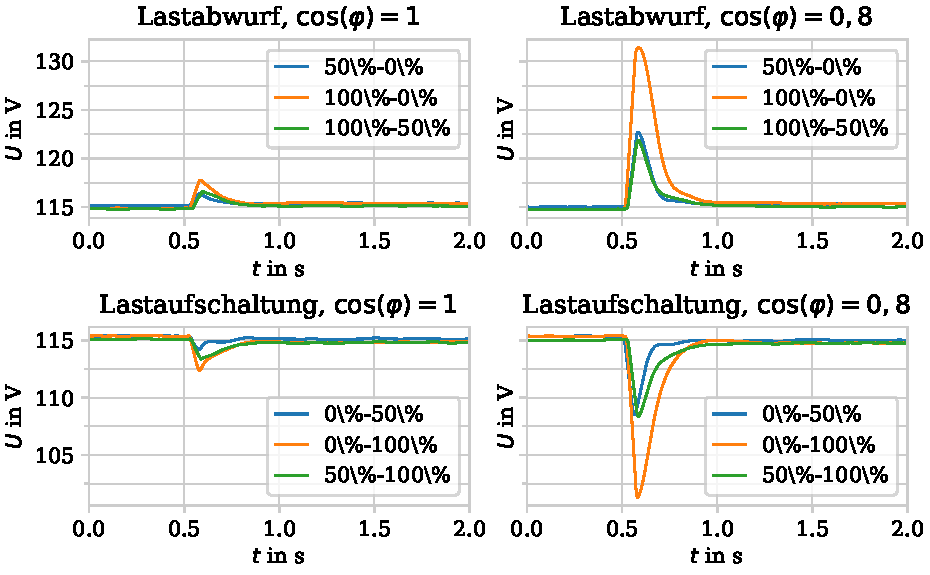
\includegraphics{Bilder/DynamischeMessung.pdf}
	\caption{Zeitverläufe der dynamischen Messung}
	\label{fig:ZeitverlaufDynamischOhneRegleraenderung}
\end{figure}

\section{Parameter und Zeitverläufe der Dynamischen Messung mit Reglerveränderung}
\label{sec:ReglerparameterDynamischeMessung}
Hinweis: Die Versuche sind nach einem System der Firma Piller Power Systems für Sonderprüfungen nummeriert.

\begin{longtable}[]{ll}
    \caption{Veränderter D-Anteil (Standardwert: $\mathrm{UgenCtrlD_G}=27648$)}
    \label{tab:Parameter-D-Messung}
    \tabularnewline
    \toprule
    Versuchnr.     & $\mathrm{UgenCtrlD_G}$ \\
    \midrule
    \endfirsthead
    \toprule
    Versuchnr.     & $\mathrm{UgenCtrlD_G}$ \\
    \midrule
    \endhead    
    9.1.1.1.1/2 & 26112        \\
    9.1.1.2.1/2 & 26880        \\
    9.1.1.3.1/2 & 28160        \\
    9.1.1.4.2 & 29184        \\
    9.1.4.6.1/2 & 256          \\
    9.1.4.6.3/5 & 5376         \\
    9.1.4.6.4/6 & 13824        \\
    9.1.4.6.7/8 & 20736        \\
    \bottomrule
\end{longtable}

\begin{longtable}[]{ll}
    \caption{Veränderter I-Anteil (Standardwert: $\mathrm{UgenCtrlI_G}=304$))}
    \label{tab:Parameter-I-Messung}
    \tabularnewline
    \toprule
    Versuchnr.     & $\mathrm{UgenCtrlI_G}$ \\
    \midrule
    \endfirsthead
    \toprule
    Versuchnr.     & $\mathrm{UgenCtrlI_G}$ \\
    \midrule
    \endhead    
        9.1.2.1.1/2 & 0            \\
        9.1.2.2.1/2 & 152          \\
        9.1.2.3.1/2 & 456          \\
        9.1.2.4.1/2 & 608          \\
        9.1.2.6.1/2 & 912          \\
    \bottomrule
\end{longtable}

\begin{longtable}[]{lll}
    \caption{Veränderter konstanter P-Anteil, eingestellt mit Begrenzung des PP-Glieds,\\Standardwerte: $\mathrm{UgenCtrlPP_G}=2048$, $\mathrm{UgenCtrlPP_{UL}}=8192$, $\mathrm{UgenCtrlPP_{LL}}=6144$)}
    \label{tab:Parameter-P-Messung}
        \tabularnewline
    \toprule
    Versuchnr.     & $\mathrm{UgenCtrlPP_{LL}}$ & $\mathrm{UgenCtrlPP_{UL}}$ \\
    \midrule
    \endfirsthead
    \caption{Veränderter konstanter P-Anteil, eingestellt mit Begrenzung des PP-Glieds,\\Standardwerte: $\mathrm{UgenCtrlPP_G}=2048$, $\mathrm{UgenCtrlPP_{UL}}=8192$, $\mathrm{UgenCtrlPP_{LL}}=6144$)}
    \tabularnewline
    \toprule
    Versuchnr.     & $\mathrm{UgenCtrlPP_{LL}}$ & $\mathrm{UgenCtrlPP_{UL}}$ \\
    \midrule
    \endhead
        9.1.3.1.1/2 & 3072         & 3072  \\
        9.1.3.2.1/2 & 4608         & 4608  \\
        9.1.3.3.1/2 & 8192         & 8192  \\
        9.1.3.4.1/2 & 12288        & 12288 \\
    \bottomrule
\end{longtable}

\begin{longtable}[]{lll}
    \caption{PI-Regler mit veränderten konstanten Verstärkungen, eingestellt mit Begrenzung des PP-Glieds,\\Standardwerte: siehe \cref{tab:Parameter-P-Messung},\\D-Glied ausgeschaltet: $\mathrm{UgenCtrlD_G=0}$}
    \label{tab:Parameter-PI-Messung}
    \tabularnewline
    \toprule
    Versuchnr.     & $\mathrm{UgenCtrlPP_{LL}}$ & $\mathrm{UgenCtrlPP_{UL}}$ \\
    \midrule
    \endhead
        9.1.3.1.1/2 & 3072         & 3072  \\
        9.1.3.2.1/2 & 4608         & 4608  \\
        9.1.3.3.1/2 & 6144         & 6144  \\
        9.1.3.4.1/2 & 12288        & 12288 \\
    \bottomrule
\end{longtable}

%\begin{landscape}
\begin{figure}[!ht]
    \centering
    \oldincludegraphics[width=\textheight-.4in, angle=90]{Bilder/MessungReglerSweep.pdf}
    \caption{Zeitverläufe der dynamischen Messung mit Reglerveränderung}
    \label{fig:MessungReglerSweep}
\end{figure}
%\end{landscape}

\section{Zeitverläufe der Spannungen aus den Parameterstudien}
\begin{figure}[!ht]
    \centering
    \begin{subfigure}{\linewidth}
        \centering
        \oldincludegraphics[width=\textheight-2.5in, angle=90]{Bilder/ParameterSweep.pdf}
        \subcaption{Hauptinduktivitäten, Statorstreuinduktivitäten}
        \label{fig:InduktivitatenSweepA}
    \end{subfigure}
    \caption{Zeitverläufe der simulierten Spannungen aus der Parameterstudie der Induktivitäten. Die Legende rechts gibt den jeweiligen Variationsfaktor einer Kurve. Aufgetragen sind 10er-Schritte aus der Parameterstudie.}
\end{figure}

\begin{figure}[ht]\ContinuedFloat
    \begin{subfigure}{\textwidth}
        \centering
        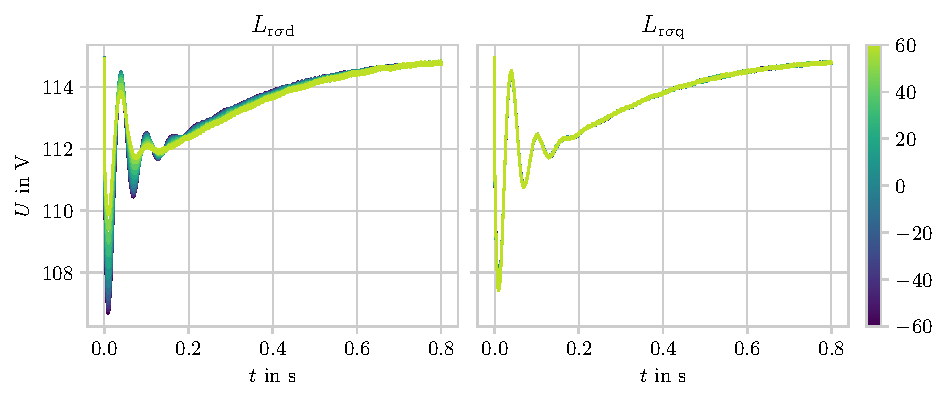
\includegraphics{Bilder/ParameterSweep_RotorStreuinduk.pdf}
        \subcaption{Rotorstreuinduktivitäten des Synchrongenerators. Aufgetragen sind 10er-Schritte aus der Parameterstudie.}
        \label{fig:InduktivitatenSweepB}
    \end{subfigure}
    \begin{subfigure}{\textwidth}
        \centering
        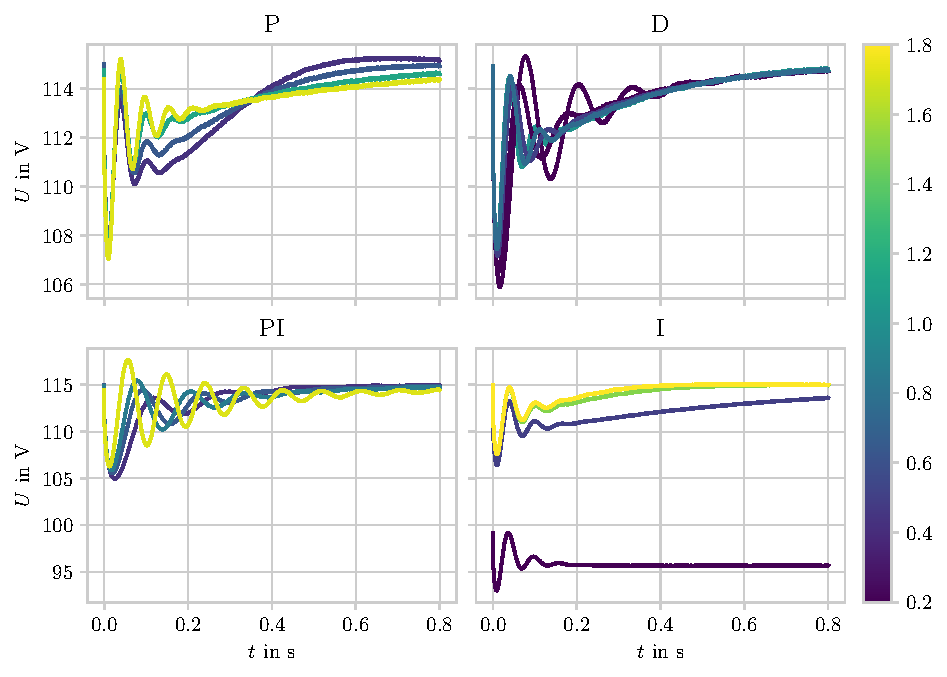
\includegraphics{Bilder/simulation_reglerSweepSpannungen.pdf}
        \subcaption{Reglerparameter. Die Legende rechts gibt den jeweiligen Variationsfaktor einer Kurve. Aufgetragen sind 10er-Schritte aus der Parameterstudie.}
    \label{fig:SpannungenReglerSweep}
    \end{subfigure}
    \caption{Zeitverläufe der simulierten Spannungen aus der Parameterstudie.}
    \label{fig:ZeitverlauefeSpannungenParametersweep}
\end{figure}

\chapter{Quellcoode}
\label{chap:Quellcode}
\definecolor{shadecolor}{named}{lightgray}

\section{Modelica-Code}
\label{sec:ModelicaCode}

\begingroup
\captionsetup{type=listing}
\caption{Record für die Maschinendaten der Asynchronmaschine\label{lst:RecordASMData}}
\begin{minted}{modelica}
within Frequenzumformer.Maschinenparameter;
record AIM_SquirrelCageData
    extends BasisDaten;
    import Modelica.Constants.pi;
    
    parameter Modelica.SIunits.Reactance X0 "Main reactance"
    annotation(Dialog(group = "Reactances"));
    parameter Modelica.SIunits.Reactance X1 "Stator leakage reactance"
    annotation(Dialog(group = "Reactances"));
    parameter Modelica.SIunits.Reactance X2 "Rotor reactance"
    annotation(Dialog(group = "Reactances"));
    
    parameter Modelica.SIunits.Resistance Rs "Stator resistance per phase"
    annotation(Dialog(group = "Resistances"));
    parameter Modelica.SIunits.Resistance Rr "Rotor resistance of equivalent m phase winding w.r.t. stator side"
    annotation(Dialog(group = "Resistances"));
    
    parameter Modelica.SIunits.Inductance Lm=X0/(2*pi*fsNominal) "Stator main field inductance per phase"
    annotation (Dialog(tab="Calculated resistances and inductances"));
    parameter Real sigma=1-X0^2/((X0+X1)*(X0+X2)) "total strey cocoefficient sigma"
    annotation (Dialog(tab="Calculated resistances and inductances"));
    parameter Modelica.SIunits.Inductance Lssigma=X1/(2*pi*fsNominal) "Stator stray inductance"
    annotation (Dialog(tab="Calculated resistances and inductances"));
    parameter Modelica.SIunits.Inductance Lrsigma=X2 / (2*pi*fsNominal) "Rotor stray inductance"
    annotation (Dialog(tab="Calculated resistances and inductances"));
    parameter Modelica.SIunits.Inductance Lszero=Lssigma "Rotor zero inductance" 
    annotation (Dialog(tab="Calculated resistances and inductances"));
    parameter Modelica.SIunits.Inductance L0 "Salient inductance of an unchorded coil"
    annotation (Dialog(tab="Calculated resistances and inductances"));

    annotation(
      Icon(coordinateSystem(extent = {{-100, -40}, {100, 100}})));
  end AIM_SquirrelCageData;
\end{minted}
\endgroup

\begingroup
\captionsetup{type=listing}
\caption{Vollständiges Modell des Frequenzumformers \label{lst:UmformerVollstandig}}
\begin{minted}{modelica}
within Frequenzumformer;

model Umformer
  constant Integer m = 3 "Number of phases";
  import Modelica.Constants.pi;
  Modelica.Magnetic.FundamentalWave.BasicMachines.SynchronousInduction
      Machines.SM_ElectricalExcited smee(IeOpenCircuit = smeeData.IeOpenCircuit, Jr = smeeData.Jr, Js = smeeData.Js, Lmd = smeeData.Lmd, Lmq = smeeData.Lmq, Lrsigmad = smeeData.Lrsigmad, Lrsigmaq = smeeData.Lrsigmaq, Lssigma(fixed = false, start = smeeData.Lssigma), Re = smeeData.Re, Rrd = smeeData.Rrd, Rrq = smeeData.Rrq, Rs(fixed = false), TeOperational(displayUnit = "K") = 293.15, TeRef(displayUnit = "degC") = 293.15, TrOperational(displayUnit = "K") = 293.15, TrRef(displayUnit = "K") = 293.15, TsOperational(displayUnit = "K") = 293.15, TsRef(displayUnit = "degC") = 293.15, VsNominal = smeeData.VsNominal, alpha20e = 0, alpha20r = 0, alpha20s = 0, effectiveStatorTurns = smeeData.effectiveStatorTurns, fsNominal = smeeData.fsNominal, m = m, p = smeeData.p, phiMechanical(displayUnit = "rad", fixed = false), sigmae = smeeData.sigmae, useDamperCage = true, useSupport = false, wMechanical(displayUnit = "rev/min", fixed = false));
  Modelica.Mechanics.Rotational.Sensors.SpeedSensor speedSensor;
  Modelica.Electrical.Analog.Basic.Ground ground;
  Modelica.Electrical.MultiPhase.Basic.Star starNet(m = m);
  Modelica.Blocks.Math.Gain frequency(k = 8 / (2 * pi));
  Modelica.Electrical.Machines.Utilities.TerminalBox terminalBox1(terminalConnection = "D");
  Modelica.Electrical.MultiPhase.Sensors.CurrentQuasiRMSSensor I_in;
  Modelica.Magnetic.FundamentalWave.BasicMachines.AsynchronousInduction
      Machines.AIM_SquirrelCage aimc(Jr = aimcData.Jr, Js = aimcData.Js, Lm = aimcData.Lm, Lrsigma = aimcData.Lrsigma, Lssigma(fixed = false), Rr = aimcData.Rr, Rs(fixed = true, start = aimcData.Rs), TrOperational(displayUnit = "K") = 293.15, TrRef(displayUnit = "K") = 293.15, TsOperational(displayUnit = "K") = 293.15, TsRef(displayUnit = "K") = 293.15, alpha20r = 0, alpha20s = 0, effectiveStatorTurns = aimcData.effectiveStatorTurns, fsNominal = aimcData.fsNominal, m = m, p = aimcData.p, phiMechanical(displayUnit = "rad"), useSupport = false, useThermalPort = false, wMechanical(displayUnit = "rev/min"));
  Modelica.Electrical.Analog.Basic.Ground groundNet;
  Frequenzumformer.Simulationsparameter simData(JRotor = 1.58, VNominal = 410, fNominal = 50, load = 0.665);
  parameter Modelica.Electrical.Machines.Utilities.ParameterRecords.SM_Electri
      calExcitedData smeeData(IeOpenCircuit = 7.2563105523832900, Jr = 0, Lmd = 131.389E-6, Lmq = 47.975E-6, Lrsigmad = 12.35031219E-6, Lrsigmaq = 9.428981013E-6, Lssigma = 16.7536222E-6, Re = 6.8, Rrd = 5.873051175E-3, Rrq = 7.587723698E-3, Rs = 0.006679333, VsNominal = 115, effectiveStatorTurns = 14.958, fsNominal = 400, p = 8, sigmae = 0.1973, useDamperCage = true);
  Frequenzumformer.Maschinenparameter.AIM_SquirrelCageData aimcData(Jr = 0, L0 = 0, Rr = 0.120, Rs = 0.083574, X0 = 14.83, X1 = 0.448208, X2 = 0.791, effectiveStatorTurns = 9.171, p = 1);
  Modelica.Blocks.Sources.Ramp ramp_net(duration = 0.5, height = simData.VNominal * sqrt(2));
  Frequenzumformer.Helper.SignalSineVoltage netVoltage;
  Modelica.Electrical.Analog.Basic.Ground groundExcitation_trans;
  Frequenzumformer.Regler.Offset_Map offset_Map(I1 = 0,I2 = 32767, O2 = 80);
  Modelica.Blocks.Math.Feedback feedback;
  Modelica.Blocks.Sources.BooleanStep controlOn(startTime = 0.7, startValue = false);
  Modelica.Blocks.Sources.Ramp V_set(duration = 0.3, height = 115, startTime = 0.7);
  Frequenzumformer.Regler.Offset_Map offset_Map1(O2 = 3888 / 256);
  Modelica.Electrical.Analog.Sources.SignalVoltage Erregerspannung;
  Modelica.Electrical.Machines.Sensors.CurrentQuasiRMSSensor I_out;
  Frequenzumformer.Helper.Multiphase.UniversalPowerSensor universalPowerSensor;
  Modelica.Electrical.Machines.Utilities.TerminalBox terminalBox(terminalConnection = "Y");
  Modelica.Electrical.Machines.Sensors.VoltageQuasiRMSSensor V_out;
  Modelica.SIunits.Torque P_out_w = universalPowerSensor.P / speedSensor.w;
  Frequenzumformer.Regler.Spannungsregler spannungsregler(Ts = 0.00078125, UgenCtrlD_D = 256, UgenCtrlD_G = 27648, UgenCtrlD_LL = -32768, UgenCtrlD_T = 2048, UgenCtrlD_UL = 32767, UgenCtrlI_D = 4096, UgenCtrlI_G = 304, UgenCtrlI_LL = 0, UgenCtrlI_UL = 32767, UgenCtrlLL = 0, UgenCtrlPP_D = 256, UgenCtrlPP_G = 2048, UgenCtrlPP_LL = 6144, UgenCtrlPP_UL = 8192, UgenCtrlP_D = 256, UgenCtrlP_LL = -32768, UgenCtrlP_UL = 32767, UgenCtrlUL = 14336);
  Modelica.Mechanics.Rotational.Components.Inertia fan(J = simData.JRotor, a(fixed = false), phi(displayUnit = "rad"), w(fixed = true, start = 314));
  Modelica.Electrical.MultiPhase.Basic.Star star;
  Modelica.Electrical.MultiPhase.Basic.VariableResistor resistor;
  Modelica.Electrical.MultiPhase.Basic.VariableInductor inductor;
  Modelica.Blocks.Sources.CombiTimeTable loadTimeTable(extrapolation = Modelica.Blocks.Types.Extrapolation.HoldLastPoint, fileName = "V:/prak/J.Pusicha/02_BA/03_Simulation/Laststufen_timetable.txt", smoothness = Modelica.Blocks.Types.Smoothness.ConstantSegments, table = [0, 0.705328, 0.00021048; 6.2, 0.352664, 0.00010524], tableName = "laststufen", tableOnFile = false);
  Modelica.Blocks.Routing.Replicator replicator(nout = 3)
  Modelica.Blocks.Routing.Replicator replicator1(nout = 3);
  Frequenzumformer.Maschinen.SM_Erreger sM_Erreger;
  Modelica.Blocks.Math.Add add;
  Modelica.Blocks.Sources.Step step(height = 10, startTime = 2.2);  
initial equation
  aimc.Lssigma = aimcData.Lssigma;
  smee.Lssigma = smeeData.Lssigma;
equation
  ...
end Umformer;
\end{minted}
\endgroup

\section{Python-Code}
\label{sec:PythonCode}

\begingroup
\captionsetup{type=listing}
\caption{Auszug aus \texttt{preprocessData.py}\label{lst:PreprocessData}}
\begin{minted}{python}
...
def zero_crossing(ndarray):
    return np.where(np.diff(np.sign(ndarray)))[0]

def freq_zero_crossing(ndarray, deltaT=1/(60e3)):
    """Gives back numpy array with current frequencys of sampled sinusoidal data by counting zero crossings.
    
    Args:
        series (series): A pandas Series containing the measured data,
        deltaT (float): Sample Time (The time between to data-points) in seconds. Default is 1/(60e3) resp. 60kHz sample freq,
    """
    data = ndarray
    # indices before crossing
    crossings = zero_crossing(data)
    # Select every 2nd Crossing beginning with the first to detect a whole period (2 zero crossings):
    crossings = crossings[0::2]
    
    freq = np.zeros(data.size)
    # Iterate only to pre last index, because index_end will use last crossing
    for i in range(crossings.size - 1):
        pre_cross_start = crossings[i]
        past_cross_start = crossings[i] + 1
        pre_cross_end = crossings[i+1]
        past_cross_end = crossings[i+1] + 1
        # Interpolate start and end Index
        index_start = pre_cross_start + (data[pre_cross_start] / (data[pre_cross_start]-data[past_cross_start]))
        index_end = pre_cross_end + (data[pre_cross_end] / (data[pre_cross_end]-data[past_cross_end]))
        period = (index_end - index_start) * deltaT 
        freq[past_cross_start:past_cross_end] = 1 / period 
        # Remember: Slicing end is **not** accessed in numpy. 
        # |--> the last value is written at 'pre_cross_end' and the next period will start immediately at 'past_cross_end'
    return freq

def period_indexes(array):
    """
    """
    return zero_crossing(array)[0::2]

def periodic_mean(array, periods):
    """Calcs mean of every periodic of input sinusoidal signal. Crossings arg have to be indexes where signal periods begin/end. Head and tail (before/after first/last period) will be overwritten with value of nearest period.
    """
    for i in range(periods.size - 1):
        past_cross_start = periods[i] + 1
        past_cross_end = periods[i+1] + 1 # past_cross_end belongs already to next period
        array[past_cross_start:past_cross_end] = np.mean(array[past_cross_start:past_cross_end])
    # overwrite head and tail with of rms of first(last) full period
    array[0:periods[0]] = array[periods[0]+1]
    array[periods[-1]+1:] = array[periods[-1]]
    return array

def dynamic_rms(array):
    """Calculates the rms value of a sinusoidal function with period detection by zero crossing **in place**, that means,
    the source array will be modified. Returns Reference to modified array.
    """
    index =  period_indexes(array)
    return np.sqrt(periodic_mean(np.square(array), index))

def active_power(u, i):
    """Calcs effective power of input voltage and current
    """
    return periodic_mean(u * i, period_indexes(u))
    
def smooth(series, n):
    """Smooths data in input series with rolling mean over n values
    """
    return series.rolling(n).mean()

def samples_per_period(delta, nom_freq):
    """Gives back Number of Samples per Period when sampling a nom_freq signal with delta 
    """
    return round(1 / (nom_freq*delta))
...
		
\end{minted}
\endgroup


\subsection{Parameterstudie}
Mit dem Paket \mintinline{python}{modelicaSweep.py} (siehe \cref{lst:ModelicaSweep}) wird die Parameterstudie an dem \textsc{Modelica}-Modell durchgeführt. Vorraussetzung ist, dass sich das kompilierte Modell \texttt{Umformer.exe} und die Begleitdateien \texttt{Umformer\_init.xml}, \texttt{Umformer\_prof.intdata}, \texttt{Umformer\_prof.realdata} und \texttt{Umformer\_info.json} in dem Arbeitsverzeichnis \texttt{model\_\-lastsprung} befinden. Über \cref{lst:ParameterSweep} wird die Funktion \mintinline{python}{run_model()} aufgerufen. Der Funktion werden ein Dictionary mit Simulationsparametern der Form 
\begin{minted}{python}
{"Parameter":Wert,
 ...}
\end{minted}
und der Dateiname der Ergebnisdatei übergeben. Jeder Aufruf von \mintinline{python}{run_model()} startet einen Unterprozess, der über den Shell-Befehl \mintinline{python}{ start / wait /min <model> -override <parameter> -r=<result\_file>} das Modell mit den veränderten Simulationsparametern ausführt. Durch den Aufruf des Unterprozesses ist es möglich, mehrere Simulationen auf verschiedenen Prozessoerkernen parallel durchzuführen.

\begingroup
\captionsetup{type=listing}
\caption{Ausführen der Parameterstudie mit \mintinline{python}{modelicaSweep.py},\label{lst:ParameterSweep}}
\begin{minted}{python}
import multiprocessing as mp
from multiprocessing.pool import ThreadPool
import modelicaSweep

simulations_parameter = [({'aimcData.X0': 3.7075}, 'aimc_X0_dp=-60'),
                         ({'aimcData.X0': 3.7941587045780443}, 'aimc_X0_dp=-59'),
                         ...]

if __name__ == "__main__":
    mp.freeze_support()
    with mp.Pool() as pool:
        result = pool.starmap(modelicaSweep.run_model, simulations_parameter)
        print(*result)
\end{minted}
\endgroup


\begingroup
\captionsetup{type=listing}
\caption{Auszug aus \texttt{modelicaSweep.py}\label{lst:ModelicaSweep}}
\begin{minted}{python}
def run_model(simulation_parameters, simulation_id):
    current_working_directory = (
        r"\model_lastsprung"
    )
    model_file = current_working_directory + r"\Umformer.exe"
    result_file = rf" -r=\results_lastsprung\{simulation_id}.mat"
    simulation_parameters = " -override " + __join_str__(
        *[key + "=" + str(value) for key, value in simulation_parameters.items()], sep=""
    )
    subprocess.check_call(
        "start /wait /min " + model_file + simulation_parameters + result_file,
        shell=True,
        cwd=current_working_directory,
    )

def plot_simulation(file_name):
    simulation = DyMat.DyMatFile("results_lastsprung/" + file_name + ".mat")
    simulation_time = simulation.abscissa('V_out.V')[0]
    voltage = simulation.data('V_out.V')
    JUMP_TIME = 2.2
    JUMP_INDEX = np.where(simulation_time == JUMP_TIME)[0][0]
    simulation_time, voltage = np.vstack((simulation_time-JUMP_TIME, voltage))[:,JUMP_INDEX:] # Combine both arrays to slice them with only one command
    return simulation_time, voltage

...
    
def r_squared(ydata, yfit):
    """ Calc R^2 of a regression by the measured ydata and the result of the curve fitting yfit
    """
    sum_square_residual = np.sum((ydata - yfit)**2)
    sum_square_total = np.sum((ydata - np.mean(ydata))**2)
    return 1 - sum_square_residual/sum_square_total

def __join_str__(*args, sep=" "):
    return sep.join(str(arg) for arg in args)

def file_name_to_list(file_name):
    """ <machine>_<parameter>_dp=<design point> |--> [machine, parameter, design point]
    """
    *machine, parameter, dp = file_name.split('_')
    machine = '_'.join(machine) # allows machine names to contain '_'
    *_, dp = dp.split('=')
    return (machine, parameter, int(dp))
\end{minted}
\endgroup

\begingroup
\captionsetup{type=listing}
\caption{Auszug aus \texttt{trendanalyse.py}\label{lst:Trendanalyse}}
\begin{minted}{python}
...
def trend(x, y, y0):
    """ Calc the average derivative of y (which is a dependent variable on x) related to y0
    """
    if not np.size(x) == np.size(y):
        raise ValueError("x and y array don't match size")
    return (y[-1] - y[0]) /y0 # / (x[-1] - x[0])

def trend_of_sequences(x, y, x0, sequences=[]):
    """ Split (x,y) in sequences and calc trend of every sequence. Sequences are given as list of tuples with x values. In Case a tuple is partly not in x the transient will be interpolated. 
    """
    if sequences:
        min_seq = min(sequences)
        max_seq = max(sequences)
        # make sure the tuples are overlapping with x:
        try:
            index_min_seq = int(np.argwhere(x < min_seq[1])[0])
        except IndexError as e:
            raise IndexError('tuple {min_seq} might be lower than x'.format(min_seq=repr(min_seq))) from e
        try:
            index_max_seq = int(np.argwhere(x > max_seq[0])[0])
        except IndexError as e:
            raise IndexError('tuple {max_seq} might be greater than x'.format(max_seq=repr(max_seq))) from e

    else:
        sequences = [(x[0], x[-1])]
        min_sequence = None
        max_sequence = None
    y0 = y[int(np.argwhere(x == x0)[0])]
    results = []
    for sequence in sequences:
        # highest index up to which x is less/equal than lower bound else lowest index of x:
        index_leq_lo_bound = np.argwhere(x <= sequence[0]) # index lower/equal lower bound
        index_min = int(index_leq_lo_bound[-1]) if index_leq_lo_bound.size > 0 else 0
        # lowest index from which x is greater/equal upper bound else highest index of x:
        index_geq_up_bound = np.argwhere(x >= sequence[1]) # index greater/equal upper bound
        index_max = int(index_geq_up_bound[0])+1 if index_geq_up_bound.size > 0 else None # NOTE: ``int(...)+1`` scince numpy _ex_cludes last element when slicing 
        
        interpol = interpolate.interp1d(x[index_min:index_max], y[index_min:index_max], fill_value='extrapolate')
        x_interpol = np.linspace(sequence[0],sequence[1],2)
        y_interpol = interpol(x_interpol)
        results.append(trend(x_interpol, y_interpol, y0))
    return results
\end{minted}
\endgroup

\begingroup
\captionsetup{type=listing}
\caption{Befehle zum Ausführen von \texttt{trendanalyse.py}\label{lst:TrendanalyseCommand}}
\begin{minted}{python}
import trendanalyse
parameter_trends = {}
for parameter, group in df_fitted.groupby(['machine', 'parameter']):
    parameter_trends[parameter] = {column : np.array([-1, -1, 1, 1])*np.array(trendanalyse.trend_of_sequences(group.loc[parameter, 'change'].to_numpy(), group.loc[:,column].to_numpy(), x0=1, sequences=[(.25,1), (.5,1), (1,2), (1,4)])) for column in group.loc[:,'v_offset':'ISE']}

df_trends = pd.DataFrame.from_dict(parameter_trends, orient='index')
df_trends = df_trends.explode(list(df_trends))
df_trends.rename_axis(['machine', 'parameter'], inplace=True)
df_trends.insert(0, 'factor', [.25, .5, 2, 4]*(len(df_trends.index)//4))
df_trends.set_index(['factor'], append=True, inplace=True)
\end{minted}
\endgroup

\backmatter
\listoffigures{}
\listoftables{}
%\lstlistoflistings{}
\printbibliography[]

\end{document}